\documentclass[12pt,a4paper]{report}

% command to compile the file
% xelatex 
% biber 
% xelatex

% choose options for [] as required from the list
% in the Reference Guide, Sect. 2.2
\usepackage{setspace}
\usepackage{fancyhdr}
\usepackage{indentfirst}
\usepackage{longtable}
\usepackage{makeidx}
\usepackage{hhline}
\usepackage{mathpazo}
\usepackage[svgnames]{xcolor}
\usepackage{pifont}
\usepackage{graphicx}        % standard LaTeX graphics tool
\usepackage{float}  % force the figure at specified location
\usepackage{multirow}
\usepackage{geometry}
\usepackage{diagbox}
\usepackage{rotating}
\usepackage{amsmath}
\usepackage{amssymb}
\usepackage{xeCJK}
\usepackage{longtable}
\usepackage{titlesec}
\usepackage{threeparttable}% tables with footnotes
\usepackage{subfigure}
\usepackage{enumitem}
\usepackage{lastpage}
\usepackage{subfigmat}% matrices of similar subfigures, aka small mulitples
\usepackage{nomencl}
\usepackage{lscape}
\usepackage[hyphens]{url}
\usepackage{caption}

\definecolor{zaffre}{rgb}{0.0, 0.08, 0.66}
\definecolor{azure}{rgb}{0.0, 0.5, 1.0}
	
\usepackage[colorlinks=true, linkcolor=Blue, urlcolor=Maroon, citecolor=magenta]{hyperref}
\usepackage[sorting=none,style=numeric,backend=biber]{biblatex}
%\usepackage[ps2pdf, CJKbookmarks=true,bookmarks=true,colorlinks=true,linkcolor=red]{hyperref}

% define a new list with no indent for itemed text
\newlist{dingautolist2}{enumerate}{1}
\setlist[dingautolist2,1]{
%  labelindent=indent,
%  listparindent=indent,
%  leftmargin=indent,
	labelindent=30pt,
     leftmargin=30pt,
     listparindent=30pt,
     itemindent=30pt,
%  labelwidth=2pt,
%  itemsep=2pt,
%  label=(\alph*),
    label=(\arabic*),
%    label=(\Alph*),
%  label=\protect\circled{\arabic*},
%  label=\protect\textcircled{\small\arabic*},
%  label=\protect{\protect\ding{\value*}},
%  start=192,
  align=left,
  itemsep=0pt,
  wide=indent,
%  itemindent=indent
%  itemindent=\dimexprindent+\labelwidth+\labelsep\relax
}

% define a new list with no indent for itemed text
\newlist{enumerate2}{enumerate}{1}
\setlist[enumerate2,1]{
%  labelindent=indent,
%  listparindent=indent,
%  leftmargin=indent,
	labelindent=30pt,
     leftmargin=30pt,
     listparindent=30pt,
     itemindent=30pt,
%  labelwidth=2pt,
%  itemsep=2pt,
  label=(\alph*),
%    label=(\arabic*),
%    label=(\Alph*),
%  label=\protect\circled{\arabic*},
%  label=\protect\textcircled{\small\arabic*},
%  label=\protect{\protect\ding{\value*}},
%  start=192,
  align=left,
  itemsep=0pt,
  wide=indent,
%  itemindent=indent
%  itemindent=\dimexprindent+\labelwidth+\labelsep\relax
}

\makeindex

% run gbk2uni *.out file between two runs of latex *.tex

% used for the subject index
% please use the style sprmidx.sty with
% your makeindex program
%%%%%%%%%%%%%%%%%%%%%%%%%%%%%%%%%%%%%%%%%%%%%%%%%%%%%%%%%%%%%%%%%%%\emph{}%%
\graphicspath{{eps/}}

\addbibresource{refs.bib}

%% rename the figure/table to 图/表
\renewcommand{\figurename}{图}
\renewcommand{\tablename}{表}

\renewcommand{\contentsname}{目录}
\renewcommand*\listfigurename{图例}
\renewcommand*\listtablename{表例}
\renewcommand{\bibname}{参考文献}

%%% set headers 
\pagestyle{fancy}
\lhead{基于价值驱动设计的系统方案权衡方法及应用}
\rhead{第\thepage 页}
\cfoot{上海交通大学}
\renewcommand{\headrulewidth}{0.4pt}
\renewcommand{\footrulewidth}{0.4pt}

% Subtract 1 from counters that are used
\renewcommand{\thesection}{\thechapter.\number\numexpr\value{section}\relax}
\renewcommand{\thesubsection}{\thesection.\number\numexpr\value{subsection}\relax}
\renewcommand{\thesubsubsection}{\thesubsection.\number\numexpr\value{subsubsection}\relax}
\setcounter{secnumdepth}{4}

%chapter1修改为第1章
\usepackage{titlesec}   
\titleformat{\chapter}{\raggedright\Huge\bfseries}{第\,\thechapter\,章}{0.5em}{}
\setcounter{chapter}{0}

\begin{document}

\begin{titlepage}
\newcommand{\HRule}{\rule{\linewidth}{0.1mm}} 
\center % Center everything on the page
 
%---------------------------------------------------------------------------------
%     HEADING SECTIONS (Enter the Homework/assignment No., only)
%---------------------------------------------------------------------------------
\textsc{\Large 上海交通大学}\\[0.5cm] % heading course Number
\textsc{\Large 航空航天学院}\\[0.5cm] % heading course name
\textsc{\large 技术报告}\\[0.5cm] % Minor heading
%---------------------------------------------------------------------------------
%     TITLE SECTION (Replace 'TITLE' with the Homework/assignment Name/title)
%---------------------------------------------------------------------------------
 
\HRule \\[0.4cm]
{ \huge \bfseries 基于价值驱动设计的系统方案权衡方法及应用}\\[0.1cm] % Title of your Homework/assignment
\HRule \\[1.5cm]
 
%---------------------------------------------------------------------------------
%     AUTHOR SECTION (EDIT THE NAME and T.NO., only)
%---------------------------------------------------------------------------------
 
\begin{minipage}{0.4\textwidth}

\begin{flushleft} \large 
\emph{编写:} 宋文滨\\
\end{flushleft}

\begin{flushleft} \large
\emph{校对:} 李少伟\\
\end{flushleft}

\begin{flushleft} \large
\emph{审核:}祁洋
\end{flushleft} 

\begin{flushleft} \large
\emph{批准:}宋文滨
\end{flushleft} 

\end{minipage}\\[5cm]

\vspace*{\fill}  % place text at the end of page 
{

\includegraphics[width=0.6\textwidth]{sjtu-logo.eps} \\[1cm]
\large \today}\\[1cm] % Date, change the \today to a set date if you want to be precise
\vfill % Fill the rest of the page with white-space
\end{titlepage}
\include{GradingRubric}
\pagenumbering{roman}
\tableofcontents          % Required
\listoffigures
\listoftables
\newpage

%%%%%%%%%%%%%%%%
%\begin{CJK*}{UTF8}{gbsn}
%\setcounter{secnumdepth}{3} \setlength{indent}{2em}
\title{基于价值驱动设计的系统方案权衡方法及应用}
\author{宋文滨}

\date
\maketitle

\newpage
\makenomenclature

%%%%%%%%%%%%%%%%
%\begin{CJK*}{UTF8}{gbsn} remove the chapter numbering before section numbers
\setlength{\parindent}{2em}
\setlength{\parskip}{0.5em}
\setstretch{1.5}

\setcounter{page}{1}
\pagenumbering{arabic}
\rhead{第\thepage 页/共\pageref{LastPage}页}

\chapter{研究背景}

商业航空效率和经济性的不断提升受益于一系列技术的不断改进,包括发动机的推进效率,机体结构效率和气动效率。涡扇发动机的广泛使用提高了飞机的航程,涵道比的不断增加大大减少了飞机的油耗水平。在过去半个多世纪的时间内,涡扇发动机的热效率从低于$0.4$提高到了$0.5$左右,起飞推力从$20$吨提高到了$45$吨,燃油消耗(Specific Fuel Consumption,SFC)下降了$30\%$,推进效率从$0.5$提高到了$0.75$。开式转子发动机的推进效率甚至可以提高到$0.9$。在未来10-20年的时间内,飞机动力系统的技术进步仍然是进一步提升飞行效率的关键技术之一,特别是纯电或混电技术的潜在应用对飞机布局、部件和系统设计,以及集成优化都提出了进一步发展的空间和挑战。

不断提升的涵道比影响到新机型布局的考虑,对现有机型的换发设计也带来了挑战。在飞机方案设计阶段需要针对不同发动机方案的优劣进行技术指标、项目进度、和经济指标等方面的综合权衡,以实现飞机和发动机制造商、系统供应商、航空公司以及租赁公司等不同利益相关方在项目周期内的共同收益,以确保整个项目取得商业成功。具体而言,针对各项技术因素的考虑需要放在全寿命周期内加以权衡和决策,将主制造商关心的制造和采购成本,航空公司关心的运营成本和维护成本,以及租赁公司关心的飞机价值进行综合考虑。其中,系统经济性设计是商用飞机经济性设计的重要组成部分,系统的设计及采购不仅仅影响到飞机的制造和采购成本,而且影响后续的维修、更换等运营成本,发动机选择对飞机总体方案和技术经济指标具有关键性的影响,对于商用飞机的经济性影响重大。

飞机型号项目中经常出现成本超支和项目延期。过去的典型例子包括波音公司的B787项目和空中客车公司的A380项目。B787的研发延迟了将近两年,并超支20亿美元的成本。空中客车A380项目推迟近两年,预算超支近20亿美元。要进行商用飞机系统经济性设计,需要有完整和成熟的方法及体系。C919和ARJ21在该项技术上是空白,宽体客机需要从一开始就进行系统经济性设计,因此急需深入研究相关的方法和流程。在本项目的第一阶段,系统开展了针对价值驱动设计(Value-Driven Design,VDD)的方法研究,建立了不同的价值模型,基于VDD的飞机方案设计流程,并以起落架方案设计为案例开展了分析。价值驱动设计主要是用于飞机概念设计阶段,是开展方案综合评估和优化的手段。但是,该方法通过对飞机项目全寿命周期内所有利益相关方所关心的评价指标的考虑,通过系统性的评估和分析方法的使用,为设计过程提供更加平衡的决策方法。

这一方法体系的发展是与飞机设计的需求密切相关的,商用飞机设计一般可以分为概念设计阶段,初步设计阶段和详细设计阶段。在实际情况中,飞机制造商通过对技术和市场的预测来分析、规划和决策未来型号的发展。如果飞机制造商能够在概念设计阶段就能够预测与判断新飞机在未来通过新环境了解新飞机在未来市场中的表现,那将是非常有价值的,同时也存在一定的不确定性和风险。新飞机的价值随着经济环境和使用环境的变化而发生变化,在传统的系统工程设计虽然强调提高对飞机需求的重视,并发展了系统的方法在项目周期内开展需求管理,但是大型项目的设计方法并没有将飞机的价值考虑在设计过程中。在微观上,飞机的经济性也没有受到设计工程师足够的重视,或者工程师缺乏有效的手段在日常设计中对决策的未来价值进行有效的考虑。因此可能一款新的机型能够很好地满足性能要求,但无法为航空公司带来具有竞争力的盈利,也无法在激烈的竞争中取得商业成功;以此需要在以往基于需求的设计方法的基础上,发展更有效的目标函数,将产品的外部价值与产品的内部设计参数相结合,提高产品价值已成为当前工程设计需要解决的亟待解决的问题。

商用飞机项目的研制中,飞机发动机之间的匹配是一项关键技术,既影响飞机的综合性能,也反映在设计成本的变化以及市场竞争力上。同时,发动机在飞机上安装问题涉及的专业数目众多,包括总体布局、气动设计、结构与载荷、使用维护,以及经济性等。传统的设计方法和流程大量依赖地面和飞行试验数据总结的经验,而随着涵道比的不断增加,翼吊布局的发动机安装问题面临越来越大的挑战,设计指标的改进空间越来越小,与此同时,不断强化的商业竞争意味着需要争取尽可能的指标优势,对设计精细化的要求大大提高。这是发展集成度越来越高的一体化设计方法的内在驱动力,一体化设计模型中综合的专业约束和设计条件的数目在增加,模型的复杂度增加,复杂模型定义中的参数需要通过分组和分级形成模型的层次化分解,以满足不同设计阶段对模型设计更改的优化需求。

在较高涵道比涡扇发动机发展的初期,发动机与飞机一般是单一关系,即:发动机是专门为某型飞机研制的,而每型飞机仅采用一型发动机。但是到了上世纪80年代中期,则开始有“一机多发,一发多机”的匹配关系。当时,为适应市场竞争的需要,在飞机和发动机研制中均考虑了如何扩大销路的问题,采取的办法是:在飞机设计中,考虑到能让航空公司有选用不同发动机的机会,即“一机多发”;而发动机研制时,也考虑到能适用于不同型号的飞机,即“一发多机”。为此,对发动机来讲,要求使用的推力范围广、附件和安装方式等的安装位置可以更换等,以适应不同的飞机。由飞机方面来看,波音 777 飞机可以选装PW4084 、 GE90 和 Trent 800这三种发动机中的任意一种。由发动机方面看,PW4000、 CF6-80C2 及 RB211—525G/H 三种发动机均既可用于波音 747-400 飞机,也可用于波音 767、空客A300等飞机。但是多选发动机也同样存在不足,会带来更高的研发费用、飞机残值受到影响等。

为了实现对多种发动机型号与飞机型号之间的一体化设计,不但需要全面的建模分析,而且需要合理的指标体系,常用的指标体系中涉及到经济性指标、技术指标、以及航空公司的运营需求。针对飞机和发动机的一体化设计,飞机制造商和发动机厂商需要在考虑航空公司市场需求的条件下,协调各自关注的利益点,最终做出是否在特定飞机型号选装特定型号的发动机。无论是单选发动机,还是多选发动机,都各有利弊。基于价值工程的理论和方法,可以提供了相对更全面的评估方法和手段,针对飞机发动机一体化设计的产业链利益相关方,建立可以涵盖多方利益的综合价值指标,并以此为评估目标,实现价值驱动设计流程和方法(Value Driven Design,VDD)。本项研究将以飞机发动机一体化设计为研究案例,综合全参数化模型、知识工程方法,建立基于价值工程的设计优化流程。

基于VDD的方法在飞机设计中的应用不仅限于飞机方案参数的优化,也涉及到飞机系统设计、供应商选择、目标市场的分析等环节,本项目拟参考在国际先进制造企业经济性设计中使用到的价值驱动设计,从而为宽体客机的系统经济性设计提供一条道路。价值驱动设计在系统价值评估中的应用能够为系统设计团队提供价值权衡维度,帮助提高飞机系统价值,降低单机成本,提升飞机整体经济性。在项目的目前阶段,研究的关注点在于飞机发动机一体化设计中的价值评估。

价值驱动设计是传统系统工程与多学科综合设计的结合,是系统工程理论的增强。应用价值驱动设计使得工程师在做出设计选择时,选择最佳设计而不是选择任何符合要求的设计,或者最有可能满足要求的设计。


\section{国内外研究现状}

在飞机型号研制中对技术经济性的考虑始终是一项重要的工作和评价方向,虽然在具体使用的方法和指标上存在一定的差异,对军机和民机项目都需要考虑这一领域的内容。在飞机项目中贯彻系统工程的理念和实践是改善设计质量和提高设计效率的关键技术之一,如果将系统工程的实践和多学科优化相结合,就形成了价值驱动设计(Value-Driven Design,简称VDD)。这一实践方法和基于模型的系统工程(Model-based System Engineering,MBSE)有共同的目标,在具体的技术实施中既有共性,也有差异,基于模型的系统工程方法的侧重点在于强调系统工程的原则与应用,而价值驱动设计更加强调如何提高具体的价值指标。

价值驱动设计的方法在一些文献中进行了介绍,其中Curren\cite{777curran2010value}系统总结了价值驱动方法的历史发展、方法论,并使用飞机结构设计作为案例开展了应用分析,Collopy和Hollingsworth\cite{53collopy2011value}对价值驱动设计领域的主要方法进行了介绍,并讨论了应用价值驱动设计可能带来的收益。价值驱动设计在飞机系统设计\cite{1313mullan2012development}、结构设计\cite{515castagne2006value},部件设计\cite{1210cheung2009aerospace},以及发动机选型中\cite{377cheung2012application}都有应用,价值驱动设计方法在卫星设计\cite{1318richardson2014incorporating},公务机设计\cite{1312downen2006methodology}和小型无人机的设计中也有应用\cite{516ferraro2012toward}。针对商用飞机项目,除了直接使用成本(DOC)这一指标之外,还需考虑全寿命周期的理念分析其价值变化,单一的DOC指标都应该应用价值驱动设计的方法和理念,从需求捕获对交付运营等。Zhang et.al提出了在需求定义阶段应用价值驱动设计的方法\cite{1267zhang2013prescriptive}。Monceaux et al.对价值驱动设计在飞机方案设计阶段能够发挥对作用,以及如何加以应用进行了分析\cite{1297monceaux2014overview}。将价值驱动设计应用于飞机概念设计决策中需要。

Ross et al.对在价值驱动设计的方法论中如何定义价值,以及不同价值定义对决策结果的影响进行了系统的分析。Mullan et al.提出了一种盈余模型(Surplus Value Model)的定义,用于价值驱动设计框架内,在制造商的设计目标和飞机的环保指标之间作出最优的设计决策。价值模型的定义对于价值驱动设计流程和结果的有效性具有关键性的影响,也进而影响设计决策,不同的价值模型可以得到不同的决策结果。价值模型的定义需要考虑商用飞机产业链中不同的利益相关方的诉求,市场环境,政策环境等外部因素。可以采用现有的飞机经济性

价值驱动设计在商业航班运营优化中也得到应用\cite{677curran2010value},其中采用的价值函数和飞机设计中的价值函数有一些不同。价值驱动设计不仅仅应该在单一的系统、部件、分系统,甚至单一的项目中进行应用,而应该在整个组织架构\cite{1128monceaux20127}和产业链内进行推广,Kwasa et al.	\cite{1310kwasa2015value}也研究了组织架构、设计流程和设计更改对价值驱动决策的影响。价值驱动设计甚至可以在非商业竞争环境中得到应用Goetzke1 et al.	针对一种武器系统提出了基于“讲价”模型的价值驱动设计方法\cite{1309mullan2011analytical},扩展了价值驱动设计方法的应用范围。Tibor将多维参数可视化方法与价值驱动设计方法结合起来,为价值驱动设计提供的可视化方法的决策支撑\cite{1302tibor2014visualization}。

\section{经济性模型的研究}

商用飞机的经济性设计指的是飞机的经济性作为飞机的评价指标之一,在满足飞机的气动,性能,环保性,安全性等指标下分析并提升商用飞机的经济性并提升其经济性。商用飞机的经济性分析至关重要,在飞机的设计环节就对飞机的经济性进行充分考虑,研究设计参数对商用飞机经济性的影响,得到具有良好经济性的飞机设计方案。

国外针对民用飞机的概念设计比较成熟的商业软件,包括Piano-X以及AAA(Advanced Aircraft Analysis)等,这些软件能够进行一定程度的经济性分析,然而这些软件在面向飞机的经济性参数优化方面仍然存在问题,与优化软件的耦合难度较大。相关的经济性模型的研究和发展为基于经济性的飞机优化设计与评估提供了方法与指标,这些飞机设计方法包括LCC与DOC 估算,其他飞机设计的相关指标如图\ref{fig_economics}所示。

\begin{figure}[H]
  \centering
  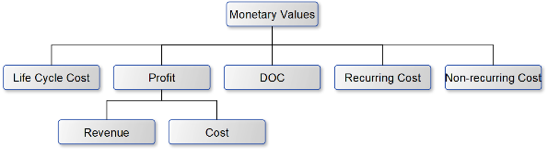
\includegraphics[width=0.8\textwidth]{./eps/economics.png}\\
  \caption{不同的经济性评价指标}
  \label{fig_economics}
\end{figure}

商用飞机的LCC为全寿命周期成本,LCC的计算需要考虑研发成本,制造成本,运营成本与处置成本。1950-1970年代,RAND发展了基于飞机空机重量的成本估算方法DAPCA IV。LCC估算方法的提出也为飞机设计提供可靠的经济性分析方法与指标。除此之外航空公司的直接使用成本DOC也是飞机经济性分析的一项重要指标。航空公司作为商用飞机的买方,将商用飞机作为盈利工具,只有飞机的盈利性足够好,才能使得达到盈亏平衡并最终盈利,从而增加航空公司购机意愿。一架盈利性良好的商用飞机,对航空公司与飞机制造商来说都是双赢。Curren 等人研究了以DOC为目标函数对飞机机身面板参数进行优化设计。飞机制造商的制造成本与研发成本同样是飞机经济性分析的一项重要指标,是飞机制造商关注的重点。Johnson以最小化LCC为目标对商用飞机的方案设计做了优化,并同时对比了分别以DOC,LCC,任务燃油,飞机起飞重量为目标函数的优化结果的不同。此外Johnson指出不同的运营参数,包括飞机的航程与速度,不同的经济性假设,包括航空燃油价格等因素,会对优化的结果产生影响。

然而这些经济性评价指标无法比较全面地对商用飞机的经济性进行分析。以DOC为指标评估商用飞机的经济性能够分析航空公司的使用成本,对其他利益相关方如飞机制造商的关切考虑不充分。以飞机的制造成本为指标能够对飞机制造商的成本进行分析,同样忽略了飞机设计方案的使用经济性。以LCC为指标评估飞机的经济性能够比较全面地考虑飞机设计的利益相关方,包括飞机制造商与航空公司,却无法对飞机的盈利性进行评估。这些经济性指标的不足促使我们对新的经济性评价指标和设计方法进行新的思考,由此发展了基于剩余价值模型的价值驱动设计方法

\section{价值驱动设计方法的研究}
基于传统系统工程的方法,设计团队缺少工程技术参数与市场需求以及更多经济性指标之间灵活的分析工具。VDD设计理念的提出始于1968年Herbert Simon的演讲, Simon指出工程设计的基本问题存在于在产品设计时,产品与实际投入使用不能很好地进行衔接,而基于价值驱动的设计能够将两者进行联系。传统设计方法的缺点之一是工程师的设计活动与产品的外在价值的相对隔离。在这种情况下,顶层设计要求并没有充分考虑产品的价值,导致产品的设计有可能偏离产品的最优设计,设计工程师也缺乏工具去直观理解设计参数的外在意义。而价值驱动设计的价值函数为工程设计参数向产品的外在价值的转化提供了可能。价值驱动设计的具体实施为工程设计提供了设计参数到产品外在价值的映射,使得工程设计活动更加具有实际意义。

上世纪90年代,在20世纪90年代,Collopy开发了一个决策理论系统工程流程,强调工程设计是一个开发有关预期产品的可操作信息并利用这些信息做出合理设计决策的过程,并强调制定价值体系以指导设计决策。在20世纪90年代后期,他还围绕价值系统设立目标函数,开发了一个基于价值进行设计的通信和控制过程。每个组件目标函数是组件属性的线性函数,(非线性)系统值模型是系统属性的标量函数,使用经济学定律进行构建。系统值模型的输出作为一项评估指标,当指标变化时,就可以衡量一个设计相对另一个设计的好坏。

2005年,美国航空航天学会系统工程科学委员会与AIAA经济学科学委员会及AIAA多学科优化科学委员会的专家一起组成了价值驱动设计委员会,用以研究价值驱动设计的方法、设计流程和相关工具,并得到了卓有成效的研究成果,一些研究成果已经应用于航空工业领域中。AIAA VDD计划委员会旨在解决所有三个技术委员会互利的重要问题。VDD委员会已经举办了多次研讨会,以展示价值驱动设计思想的应用。具体的案例如在2006年的研讨会中,价值驱动设计应用于全球定位系统的设计。Collopy和Hollingsworth 描述了价值驱动设计中的思想和方法。Eveker提出价值驱动设计的特征是工程师在做出设计选择时,选择最佳设计而不是选择满足或者虽有可能满足要求的设计。建立VDD框架的一个挑战是价值目标函数的建立,系统必须具有整体系统的目标函数,Keeney称之为价值模型,或者在工程领域中称为系统值模型,价值模型以系统属性为输入并输出对系统的评价分数。Mullan等人提出现有的价值驱动设计相对于传统的系统工程方法若要有所不同,必须也同时考虑子系统级别的相互影响,而不仅仅是不同系统级别的相互影响,并提出计算子系统相互影响的方法,并对子系统交互的重要性进行排序。结果表明孤立地分析子系统会带来决策的不准确。Isaksson等人介绍了价值驱动设计的方法与工具,指出该方法可以降低成本与风险。Monceaux等人指出传统的系统工程并没有真正意义地对设计参数进行系统性与全面性的权衡与优化。

价值驱动设计在实际的运用中也取得了重大进展。美国国防高级研究计划局(DARPA)对以价值为中心的设计进行研究并应用于F6分馏航天器。F6项目以价值为中心,该设计的重点在于量化航天器灵活性和稳健性,搭建层次化的架构分析其价值[15]。Brathwaite等人为通信卫星开发了以价值为中心的框架,并通过蒙特卡洛模拟市场的不确定性,并将其转化为卫星价值的不确定性,最终得到的结果是帕累托最优的卫星设计方案组合。Castagne等人将价值驱动设计方法应用于客舱面板的设计和优化。结果表明以不同价值函数对设计参数的优化得到不同设计结果,并且价值驱动设计可以同时为飞机制造商和航空公司带来收益。Cheung等人研究了价值驱动设计在航空发动机的优化设计的实施。相关的研究表明价值驱动方法能够与飞机设计相结合,并得到价值最优的设计。Keller等人根据月球采矿车的属性,包括月球采矿车的重量,成本,可靠性以及推进效率,建立价值模型。对月球采矿车进行评估。该价值模型包括性能模块,任务模块并考虑了NPV,并应用于系统权衡研究,技术评估与设计优化。除此之外,相关学者也对SysML系统建模语言与MATLAB结合对基于价值的设计的好处进行了研究。Collopy和Consulting等人介绍了价值驱动设计的必要性,并为全球定位系统建立了一个优化卫星总线设计的目标函数。

\chapter{研究目的}
本项研究的目的是针对长航程宽体商用飞机方案设计中的总体参数优化,主要系统和发动机选型中如何应用价值驱动设计提高飞机设计的经济性和竞争力,建立价值驱动设计流程,发展多种价值模型并开展对比分析。在此基础上,采用起落架系统和动力装置为典型案例,开展方案参数影响分析。


\chapter{主要研究内容}

价值驱动的设计(VDD)流程首先是多学科设计在飞行器研制中的应用,同时也是多指标评价方法的应用,包含了价值函数的多学科优化和多指标评价构成了VDD的基本框架。

\section{宽体飞机及发动机需求分析}

航空技术和型号的发展具有长期性,既说明了面向未来型号发展开展需求分析的必要性,也显示了其中存在挑战和不确定性,对新技术的研究既涉及到该项技术的工程可用性,也需要解决研发风险、经费、时间和市场变化等方面存在的不确定性。开展中长期的技术经济分析与需求捕获具有重要的意义,也需要系统性的方法。

包括空客\cite{Airbusgmf},波音\cite{Boeingcmo},商飞\cite{comacmf}在内的各大飞机制造商每年会发布针对未来20年的市场需求预测报告,其中按照市场细分原则提出各自对未来市场需求的预测数据。这些市场预测报告既反映了制造商对商用飞机未来市场需求的看法,也影响各制造商的潜在产品发展战略。例如庞巴迪(Bombardier) 发布的未来市场预测中\cite{bombardier},特别强调60到150座之间的“小飞机”对于航空公司开拓未来市场、提高盈利水平所能够发挥的重要作用。除此之外,一些主要的研究机构和行业协会也从技术发展趋势,行业政策,和公众需求等角度提出各自的预测报告,一些典型的报告包括NASA通过与工业界、学术界联合开展“环境友好航空(Environmentally Responsible Aviation)”项目发布的一些概念研究和技术预测(\cite{nasa, nasa2})。

未来机型分类将大致延续目前各制造商的分类方法,按照支线飞机,单通道飞机,和双通道飞机三大类别,但是将根据市场需求的变化出现更加细分的市场,例如介于三种类型之间的过渡机型,城市内的“飞行汽车”概念,超音速旅客机等,虽然A380飞机将仍然在未来20年民航市场上发挥作用,但是超大型飞机显然已经失去了市场动力。更高效率、更加环保,更加安全,支持更加灵活的运营模式的机型仍然是航空公司对未来机型的核心指标需求。

如前所述,航空市场的预测不同于其他消费品市场需求的预测,也不同于一般工业品和汽车行业的预测和需求发展,需要关注一段时间内的宏观因素变化。但是,技术决策和设计决策一旦作出,将很难改变,具有战略性和长期性的影响。市场因素的驱动将导致航空公司对飞机的盈利能力从机队的宏观盈利能力到更加关注单座的盈利能力,按照国际航协(IATA)的报告\cite{iata},航空公司在2017年预计每位乘客盈利7.69美元,比2016年的9.13美元和2015年的10.08美元有所下降。航空业2017年的平均净利润率为4.2%,低于2016年的4.9%。航空公司通过大幅折扣票价以填补空座,更加广泛的提供增值服务。 在某些地区,即使是票价大幅折扣也无法填补过多的飞机座位。 预计这种趋势将持续,因此航空公司更多关注运力管理。这说明尽管飞机制造商在目前的机型研制中对对更大的机型的关注与航空公司的实际需求存在不一致的地方。对于中国市场,虽然市场运力持续增长,上座率水平和国际平均水平基本一直,也说明聚焦单座盈利能力能够带来的收益或许更大于机队总体盈利能力的增长,也就是说飞机的大小并不是目前影响盈利水平的主要因素,也说明将单座盈利水平加入价值评价指标体系的必要性。

针对中国市场而言,区域化城市群经济区一体化战略(包括珠三角,长三角,和京津冀)的提出自然对区域间交通需求和基础设施布局产生影响,高铁网络的完善和服务的持续改善也对1000公里以内的航空运输提出了新的挑战,对旅客运输和货物运输的影响可能会出现差异化影响。一带一路战略的国际化战略和国际“逆全球化”趋势的扩散对航空市场需求和产业链发展都可能带来潜在的影响,在未来机型和机型发展规划的制定中成为不可忽略的外部因素。因此,开展需求分析,特别是中长期的需求分析需要对宏观环境变化有准确的把握,技术突破,地缘政治环境,政府社会经济政策,环境等都是影响航空业的重要因素。IATA报告通过广泛的调研和分析\cite{iata2035},梳理了可能影响2035年代商用航空市场的50个驱动因素,并将其归为11个主题(themes),在此基础上,提出了四种具有鲜明特征的宏观场景的演变(分别为新前线,可持续发展,世界政经板块演变,资源战争)。商业航空的全球性特点意味着其发展收到这些宏观因素的深刻影响,IATA报告提出了从11个主题领域提出了23项建议,可以作为未来场景定义的参考,这些因素对于未来技术,特别是战略技术的发展具有深远的影响。
\begin{table}[h]
\caption{商用航空运输业面临的主要挑战和应对建议(基于IATA报告整理\cite{iata2035})}
\label{table:iatatable}
\small
\begin{tabular}{|p{2.5cm}|p{5.5cm}|p{5.5cm}|}
\hhline{|===|}
主题 & 主要因素 & 相关建议  \\ \hline
地缘政治 & 现有国际组织作用的弱化,以及新型国家发言权的强化,国际标准的演变 &   1)增加现有国际组织的作用,提高其包容性;2)与新型国际组织加强对话与合作; 3)进一步推动民航市场的自由化发展;4)强化危机应对机制;\\ \hline
非洲与亚太 & 非洲与亚太在全球经济的份额增加;高铁等其他交通方式的影响;二线机场的财务困境  & 5)加强与亚太与非洲的利益相关方的交流;6)提高非枢纽机场的作用;\\ \hline
安全与边界& 开放边界与区域局势的相互影响;传染疾病控制;特定药物管控 &  7)全球疾病防控对航空运输业的挑战;8)建立全球生物黑客防控体系 \\ \hline
环境问题  & 航空运输业持续增长对环境的影响; &  9)环保指标是下一代航空技术和产品发展的必选项;10)航空业在环境保护方面强化全球标准的建立 \\ \hline
经济发展  & 全球经济发展中的不确定性因素;后碳能源时代的经济发展;高技术人才培养 & 11)航空产业健康发展的预警系统;12)重视航空行业教育与培训  \\ \hline
数据 &  大数据对航空产业的影响;忠实客户计划的发展;供应链管理模式;& 13)提升航空业中的乘客等大数据管理和运营能力; 14)区块链等新型数据和无线移动网络技术发展对供应链业态的影响\\ \hline 
隐私与信任  & 航空运输业各环节的安全挑战; 网络安全;&  15)新技术环境下的安全措施;16)5G时代的航空业的数据和信息安全问题;\\ \hline
技术创新 & 共享和后共享经济时代对航空业对影响;半自主和全自主技术的发展;5G时代VR/AR技术对旅行需求的影响;未来机场等基础设施的演变 & 17)多种交通模式一体化模式的发展;18)全自主技术在全产业链和全寿命周期中的应用; 19)全球范围内基础设施发展的协同;20)基础设施利用率的提高\\ \hline
价值观与社会 & 消费模式的转变带来的挑战和机遇;消费人群的变化和社会形态的演化;乘客体验; & 21)应对社会老龄化对航空旅行需求演变 ; \\ \hline 
政府作用 & 基础设施改善与新建的资金和决策挑战;金融和安全风险管理; 军民融合发展挑战; &  22)航空业持续发展对资金的需求;\\ \hline
商业模型 & 创新驱动的新机遇;全球人口结构变化带来新的消费人群的观念和需求变化; &  23)新型市场国家消费者对航空旅行预期对改变\\ 
\hhline{|===|}
\end{tabular}
\end{table}

具体到中国环境,按照IATA的报告中提到的两大主要因素都是有利于航空业的持续发展,按照IATA在2018年的预测报告\cite{iata},未来二十年(2017年至2037年),超过半数的新增旅客来自亚太地区,2037年客运总量为70亿人次。其中的主要特点表现在:
\begin{dingautolist}{182}
\item 2024年至2025年左右,中国将取代美国成为全球最大航空市场(根据飞抵、飞离中国及中国国内客运量计算)。中国经济转型为消费主导后,将长期带动客运需求强劲增长。
\item 印度位列美国之后,将在2024年左右超过英国成为第三大航空市场。
\item 印度尼西亚表现出色,在2017年跻身第十大市场,预计将在2030年跃居第四大市场。
\item 泰国将在2030年取代意大利,跻身前十位。
\end{dingautolist}

亚太地区商业航空业持续快速增长的第二个因素是基础设施投资的稳健性、长期性和战略性,按照中国民用运输机场布局规划\cite{china-airports},截至 2015 年底,我国共有民用运输机场 207 个;到 2025 年,在现有(含在建)机场基础上,新增布局机场136 个,全国民用运输机场规划布局 370 个(规划建成约 320个)。这些机场的定位和基础设施条件是考虑不同机型设计的重要参考数据,

%\textcolor{red}{按照其发挥的作用,可以分为国际枢纽,国内枢纽,区域机场,以及通用机场四个层次,需要进一步的分析。}

与此同时,航空业致力于从2020年开始实现碳中和增长,到2050年将二氧化碳排放量降至2005年水平的一半。这些指标的实现在很大程度上依赖于技术创新的发展。结合我国的实际国情和发展特点,在机型需求分析中,既需要考虑国际通行的、一般性的市场因素,也需要考虑国家战略需求和快速发展带来的机遇,同时还需要考虑缺乏必要的技术储备所带来的挑战。

建立从宏观因素到微观因素(座位数等)在飞机需求分析方法中的作用,方法流程图,具体实现方法。制造商希望推出更大的机型,增加市场和运营灵活性,也提高飞机售价和利润率水平。但是,更多的座位对航空公司的盈利能力带来挑战。将航空公司的盈利模型与飞机的设计参数,外部环境,技术趋势等因素都综合起来,形成比较综合最优的设计方案有利于整个行业的可持续发展。

对航空公司来说,每座公里收益,人员成本,航油价格,运力管理,外部环境包括竞争态势,航线网络结构,消费者消费特点的变化(客户忠诚度),机队结构,航班频率,增值服务,最直接的是就是价格,例如美国市场一些显著的特点包括低成本航空公司的快速发展,类似Frontier和Spirit等公司利用最新的、高效率的A350和B787机型在跨大西洋航线市场提供超低经济舱票价,而可以预期的超音速50座级旅客机投入商业运营对公务舱乘客带来影响。因此,探讨超级经济舱和经济舱的两舱布局或许也不是完全没有意义的事情。而对于中俄之间,航空运输增量市场有限,属于开放程度有待进一步提高的航空运输市场。

飞机的关键技术指标可以分为主要包括燃油效率和环保指标(包括噪声和排放),飞机技术水平的提升,包括更远的航程,巡航高度优势,更好的低速性能,低噪声,更舒适的客舱布局,更好的货仓处置办法,系统可靠性的提升,结构寿命的延长等,可以带来阻力下降和重量减轻的结果,进而降低燃油消耗。

对于飞机制造商而言,飞机项目的主要评价方法除了上述涉及飞机本身的技术指标以外,还包括项目投资,项目周期,盈亏平衡点(飞机架数和年生产率),市场占有率,技术水平,战略优势等内容。

\subsection{宽体飞机现状分析}

自从2010年以来,经济增长不平衡,汇率和商品价格波动,以及对国际贸易和人员自由流动的担忧。虽然这些发展可能意味着航空旅行增长较慢,但事实恰恰相反。自2010年以来,全球衡量旅客运输量的综合性指标收入客公里(RPK)平均增长率为6.7%,远高于过去三十年每年5%的表现。由于收入增加,新兴市场的人们有更多的旅行机会,伴随着航空业竞争加剧导致服务质量提高和价格下降。根据市场统计数据估计的未来趋势表明,未来二十年商业市场的需求预计将增加一倍以上。

为满足这一需求,在役机队将以3.4%的平均年增长率增长,服役的喷气式飞机数量几乎翻倍至50,660架。根据航空旅行需求增长趋势,波音公司预测,到2038年,大约40%的新飞机将交付给亚洲的航空公司。另外40%将交付给欧洲和北美的航空公司,剩下的20%将交付给中东,拉丁美洲,俄罗斯和中亚以及非洲的航空公司。然后将分析方法应用于中/远程宽体飞机的情况。为了开展预测,首先需要建立针对宽体飞机的数据库,并包含针对数据进行分析的手段,表\ref{someaircraftdata}中给出了一些宽体飞机的主要型号,例如可以将数据按航空公司或飞机类型等标准进行过滤。

Dozic和Kalic提出的三阶段的机队规划模型在第一阶段根据给定航线网络的飞机大小确定了一个近似的机群组合。根据路线市场的需求和距离,为每个目的地分配小型或中型飞机。根据第一阶段规定的航线特定机群组合,在第二阶段确定所需的飞机数量。然后在第三阶段确定飞机类型以最佳方式满足市场要求。还有一个两阶段DEA总效率方法来确定影响航空公司效率的因素\cite{repko2017scenario}。DEA是一种线性编程技术,用于根据观察到的数据评估组织或决策单位(如航空公司)的相对绩效。因此,航空公司的相对业绩定义为其产出相对于其投入的加权总和。权重不是预先确定的,而是由模型分配的,避免了由主观分配的权重(例如分析层次结构过程)引起的偏差。一般来说,DEA生产前沿可以在规模收益不变(CRS)或规模收益可变(VRS)的替代假设下,以输入或输出为导向进行非参数化操作。

\begin{table}[ht!]
\centering
\caption{一些宽体飞机型号}
\small
\begin{tabular}{|p{2.5cm}|p{2.5cm}|p{6cm}|}
\hline \hline 
飞机种类 & 航线种类	& 飞机型号 \\ \hline
宽体客机 & 长程航线	&B747, B767, B777, B787; A300, A310, A330, A340, A350, A380;MD-11, DC-10;  ILYUSHIN, Lockheed L-1011\\ \hline
\hline
\end{tabular}
\label{someaircraftdata}
\end{table}

在第二阶段回归模型中,采用了传统的无偏校正效率评分。由于还想在审查面板数据集中控制跨公司和时间错误,因此使用以下随机效应Tobit回归模型:
\begin{equation}
y_{it}=\alpha+\beta_1 A\_S1_{it}+\beta_2 A\_S2_{it}+\beta_3 S\_L_{it}+ \beta_4 F\_A_{it}+\beta_5 A\_F_{it}+v_{it}+u_i
\label{eq:prediction}
\end{equation}
式中,$y_{it}$是相关年份中各航空公司的VRS效率得分,$A\_S1_{it}$表示该航空公司的净吨公里(作为其大小的代表),$A\_S2_{it}$表示平均座位数。在相关年份相关航空公司服役的飞机,$S\_L_{it}$表示航空公司飞机飞行的平均航段长度,$F\_A_{it}$反映其机队的年龄,$A\_F_{it}$代表不同飞机系列的数量。


\subsection{影响飞机机型选择的因素分析}

航空公司的机型选择由市场需求决定,飞机制造商根据世界范围的市场需求来确定新机型的具体参数,以尽可能满足更多航空公司在不同航线结构和需求强度下的需求。在制造商及行业协会提供的航空运输市场的预测报告中,比较具有共识的意见是世界航空运输发展将基本保持$5\%$左右的增长速度,需求的增长需要不断提高的运力水平来满足,既可以通过更换使用更大的机型,也可以增加航班频率,或者改善基础设施(扩建或新建机场/跑道等)来实现。空客A380的案例事实证明,空客公司应对国际枢纽机场航班时刻紧张的解决方案并没有实现其预期的目标,即使通过换发来提高燃油经济性,也仍然无法说服航空公司采购更多A380飞机。亚太地区更倾向于通过增加基础设施投资来扩大机场容量,与此同时,一些主要的目标航线上乘客的增长率无法提供更大的机型所需的乘客数。更合适的、相对较小的机型,辅以更灵活的航班时刻,似乎能够为航空公司提供更好的选择。除了在一些需求很高的特定航线上(例如京沪航线),由于航班时刻紧张而导致的运力边际收益的损失,不足以说服航空公司引入更大的机型。一般来说,单通道飞机的航程不超过6000公里(例如B737-700: 6230 公里, A320: 5700公里)),双通道飞机的航程一般超过10000公里(B777-300: 11029公里, A330-200: 12500公里)。

单条航线的需求预测分析方法,航线网络结构对需求的影响。对于单条航线来说,影响机型选择的主要因素包括航段距离,旅客和货运需求,竞争水平,基本不会受到机场类型特征(枢纽机场或地区机场的影响)。在现有航线上,航空公司提高运力的方法包括增加航班时刻,提高上座率,更换更大的飞机(类似京沪航线上宽体飞机已成为常态),提高上座率对航空公司改善盈利是最有利的措施。


\section{飞机发动机一体化设计}

飞机发动机一体化设计涉及到多个层面的问题,在方案设计阶段,需要考虑布局选择,总体参数之间的匹配,发动机选型等内容。气动设计中需要考虑发动机安装优化,系统设计中考虑发动机和飞机的系统接口设计,结构设计中考虑挂架结构设计。选择满足飞机设计要求的航空发动机是飞机整体方案设计早期阶段的重要任务之一。 这些任务涉及飞机和发动机参数的组合。许多研究人员研究了军用飞机发动机的选择,少数研究人员研究了商用飞机发动机的选择。 例如,Eschweiler\cite{eschweiler}等人考虑到开发周期早期的性能,生命周期成本和武器系统有效性之间的相互作用,开发了一种发动机选择方法。Dugan\cite{dugan1972engine}说明了用于选择运输类飞机的发动机的程序。他指出,选择发动机的问题是选择发动机参数,包括发动机尺寸,以满足所有约束条件并最大限度地提高飞机性能。

\subsection{飞机总体方案设计方法}

在经过市场调研与确定的顶层设计需求,通过确定一组飞机设计参数定义一架飞机的完整方案,这些设计参数包括机身参数,起落架参数,短舱与发动机参数,航程与载荷,机翼参数,平尾与垂尾参数。通过飞机总体设计的经验公式对这些设计参数进行多属性的计算与评估,并进一步优化设计方案。商用飞机概念设计阶段飞机的多属性评估包括飞机的气动性能,重量,性能,环保与经济性,不同的方面的属性的计算与分析会对飞机的最终的设计方案的权衡与优化产生影响。同时在对飞机进行属性计算时需要考虑不同学科之间的耦合,比如飞机的性能会对飞机的油耗产生影响,进而影响飞机的经济性。图\ref{fig_vdd_aircraft}是飞机的概念设计阶段的设计流程与各个模块之间的关系。

图\ref{fig_vdd_aircraft}中该飞机设计流程以飞机的设计参数以及场景条件作为输入,并对飞机进行多学科分析,所用的分析方法采用经验公式的方法。对于飞机重量的估算采用两种方法结合使用,首先通过Raymer的重量估算方法进行基于飞行任务的初步MTOW估算;通过Torenbeek方法对每个飞机部件的重量进行计算并得到飞机的MTOW以及空机重量,所用的参数为飞机的设计参数。根据飞机的详细外形参数对飞机的气动参数进行基于经验公式的估算。其中根据飞机的各个部件在特定运行条件下以及特定构型对升力的贡献计算升力系数,得到全机的升力系数;飞机的阻力系数计算包括压差阻力,干扰阻力,摩擦阻力,诱导与激波阻力,按照飞机的各个部件对上述阻力的贡献进行计算并得到全机的阻力系数。根据飞机的初始设计参数以及计算得到的重量参数与气动参数对飞机的性能以及操纵稳定性进行估算,包括飞机的起飞与降落性能,飞机的巡航性能以及飞机的操纵稳定性。飞机的经济性估算包括成本与收益的计算,经济性的估算与飞机的各项属性相关,这些属性包括性能,气动与重量。根据飞机的特定运行环境,包括飞机制造商,发动机制造商以及航空公司的运营参数,宏观的经济环境包括燃油等影响参数,飞机的设计参数以及上述飞机各项属性的计算结果,根据RAND公司的DAPCA模型对飞机的LCC进行计算与欧洲AEA的DOC模型对飞机的经济性进行计算。

\begin{figure}[ht!]
  \centering
  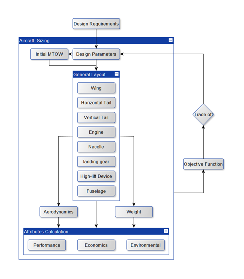
\includegraphics[width=0.8\textwidth]{vdd-aircraft.eps}\\
  \caption{基于VDD的飞机方案设计基本流程}
  \label{fig_vdd_aircraft}
\end{figure}


\subsection{发动机总体设计方法}

发动机总体设计需要同样需要采用多学科概念设计方法,该方法综合考虑了多种不同学科:发动机性能,发动机空气动力学和机械设计,飞机设计和空气动力学性能,排放预测和环境影响,发动机和机身噪声以及生产,维护和直接运营成本。多学科发动机仿真工具的最新技术是由一组扩展的工具代表的,这些工具包括:NPSS(数值推进系统仿真),WATE(涡轮发动机重量分析),FLOPS(飞行优化系统),以及ANOPP(飞机噪声预测程序)。NPSS可以处理不同级别的建模保真度,从简单的热力学循环计算到完整的3D全发动机CFD(计算流体动力学)模拟\cite{lytle2000numerical}。WATE\cite{tong2008an}是一种面向对象的计算机代码,可用于在组件级别预测不同燃气涡轮发动机配置的尺寸和重量,基于NPSS的循环参数。FLOPS\cite{mccullers1984aircraft}是可使用来自WATE和NPSS的信息进行飞机选型和任务分析的飞机概念设计代码。ANNOP\cite{kontos1996improved}是一种发动机和机身噪声预测代码,可以根据FLOPS提供的飞机尺寸和NPSS和WATE提供的发动机信息,预测认证噪声水平和噪声功率距离曲线。之前已经有不少学者成功地将这些代码整合在一起,并在飞机系统级产生发动机设计结果。

EDS(环境设计空间)工具是上述方法的衍生工具。该工具主要包括NPSS,WATE,FLOPS和ANNOP代码以及各种排放预测方法的集成。EDS提供了在不同政策和技术方案下估算潜在的未来飞机设计的源噪声,废气排放和性能的功能。EDS是称为ETS的一大套工具的一部分,目的是更好地了解噪声和不同类型的废气排放之间的关系,以及提供数据驱动决策所需的成本效益分析能力对长期和全球立法。

Genesis是一款燃气轮机的气动和机械设计工具,可用于定义基本的发动机几何形状,以及使用基于实际制造商的发动机数据库的相关性来预测发动机的重量和成本。 Jones等人\cite{jones2003a}提出了利用Genesis和燃气轮机性能工具RRAP(Rolls-Royce Aerothermal Performance)以及其他代码的混合组合的军用发动机的初步设计过程。 用于在设计过程中快速定义和完善燃气涡轮发动机,该过程考虑了发动机性能属性以及生命周期成本(TLC)。

用于燃气轮机初步设计的另一个软件包是MOPEDS(模块性能和发动机设计系统)。Jeschke等人\cite{jeschke2004preliminary}对此进行了详细介绍。该工具可以考虑所有主要燃气涡轮发动机组件及其相互关系来执行多学科和多点分析。系统还可以处理从初步设计阶段到详细设计阶段的过渡,并将初步设计结果转移到更高保真度的1D和2D模型中,以进行详细的组件设计。

GISMO软件,如Avellan和Gronstedt\cite{avellán2007preliminary}介绍的是用于飞机和发动机概念设计和分析的通用仿真和建模环境。首先使用GeSTPAn(通用平稳和瞬态推进分析)代码进行发动机性能和重量预测,然后将结果传输到飞机设计模块以进行进一步分析;这是一个反复的过程,在每个循环中都要重新设计发动机和飞机,并重复进行直到满足所有设定的飞机性能要求。

\subsection{飞机发动机一体化建模}

随着飞机方案设计阶段的技术工作越来越精细,设计手段不断提高,对飞机参数的选取优化、部件分析工作越来越繁杂,传统的几何外形建模方式和过于简单的参数化建模已经难以完全满足方案阶段飞机参数优化和部件选型对几何外形的要求。对于飞机发动机一体化设计,建立一套物理几何意义明确、外形参数驱动的全参数化建模系统,对于飞机越来越精细的方案设计对飞机外形的需求有重要意义。随着飞机总体多学科设计优化(MDO)和一体化设计的不断深入,参数化CAD模型不仅为各种方案比较和多种气动特性的研究提供了清晰无误的表达方式,而且为各学科的分析和优化提供一个高精度高质量的几何模型。

飞机短舱三维模型的建立是飞机发动机一体化设计中的一个重要环节,短舱三维模型不仅为各学科设计提供了一个统一的外形模型,更是各学科展开设计工作的基础部分。然而在一些学科基于三维模型展开设计的过程中,需要对短舱模型外形尺寸、结构布置做出相应的调整,比如在做结构拓扑优化,或是气动外形优化、减重优化、静力分析等优化设计时,可能要短舱尺寸、吊挂位置、发动机个数进行三维模型的修改。修改模型的工作十分复杂,有时甚至无法修改。以及会遇到建模方式虽然完全相同,但仍要做大量重复性工作的问题。1996年美国举办了以“快速设计与制造”为主题的专项学术讨论会,由此“快速设计”理论、方法与技术开始成为世界各国研究的热点。为了缩短建模、变换、优化分析综合流程的周期,基于计算机辅助设计软件的二次开发技术为飞机短舱模型参数化设计方法提供了一种有效的途径。采用此途径,利用模型的参数化描述以及三维模型的快速生成技术,很好地解决了这一问题。参数化建模不仅可以提高建模效率,还能很好地改善模型质量。基于特征的参数化造型设计就是建立在实体造型特征和参数化设计基础之上并将它们有机结合起来的一种方法,这种方法更适合计算机集成制造系统的产品设计。同时,参数化设计技术和特征技术作为当前CAD技术的研究热点,将二者有机结合起来形成的基于特征的参数化造型技术族更是在目前CAD/CAM/CAPP集成系统发展中的重要手段。

飞机外形复杂,如何用一组较少参数来比较精确地描述飞机外形是一个难点,也是需要持续开展深入研究的重点之一。在目前研究中多采用了样条方法(如NURBS)来描述飞机外形。虽然NURBS方法能较精确地描述飞机外形,但所需控制参数太多,且参数缺乏明确的物理意义,不便于在概念设计中获得有效的应用。Kulfan等针对这些问题提出了一种基于形状函数/分类函数变换的参数化方法(Class function /shape function Transformations,简称CST),以翼型弦向控制点处的厚度为控制参数,建立翼型模型。形状函数具有简单解析解,可以较好地对几何外形进行描述,而且可以直接控制飞机外形的几何参数。类函数是用来概括各种各样几何外形的函数,通过形状函数和类函数的结合,得到了一个用来描述几何外形具有综合性质的函数,此函数可以用来描述任意的二维图形。这种方法的优点是参数具有明确的几何含义,所需控制参数较少,适用性强,建模精度较好。对于飞机的参数化设计,湛岚等人应用这种基于形状函数和分类函数变换的参数化方法,建立客机了的机翼、尾翼、机身、短舱外形的参数化数学模型,并研究了机身与机翼连接处鼓包外形模型和定义部件位置的参数化模型,最终建立了客机全机外形参数化数学模型。然而这只是建立了一个简单的飞机外形模型,进一步研究复杂机身的参数化建模,还需要提高建模精度,对于飞机模型的细节部分缺乏进一步的描述,缺乏对飞机方案设计优化中需要考虑的大量工程约束细节。

对于发动机短舱的参数化设计,有周洪升采用了椭圆公式模拟短舱的外形,然而这样的短舱造型过于简单。上海飞机设计研究院的单文娟对某型发动机短舱进行了初步参数选取和气动外形设计;并在此基础上开展了数值仿真计算,然而其建立的短舱为一维旋转体模型,与实际的短舱仍有较大差距。强旭浩等人采用二次曲线及三次曲线对短舱进行建模并对短舱型面进行光滑性连续性的分析。曲面设计有型函数法、样条法、偏微分方程法、网格点法等,但这些方法都各有缺点,要么难以保证局部曲面的控制,要么数据计算量很大,表面网格生成困难。样条曲面方法是少有的能够各方面兼顾的参数化方法,在局部曲面控制、控制点数量、表面网格变形方面有较强的优势。而且,NURBS(Non-Uniform Rational B-Spline,非均匀有理B样条)是一种基于自由型面B样条和初等解析曲面表述相结合的几何建模方法,现已成为STEP标准中自由曲线、曲面唯一表述形式,广泛应用于CAD/CAM和计算机图形学等工程研究领域。马晓永等人针对翼吊布局飞机复杂气动外形,建立了基于样条(NURBS,非均匀有理B样条)曲面和曲面叠加技术的曲面变形方法。在对样条曲线性质分析的基础上,以某型飞机为实例,对其机翼翼根、短舱挂架局部进行曲面网格变形,结果表明该方法能有效表述其复杂几何外形及型面变化特性,并且具有较好的局域性、可控性和光滑性。NURBS曲面的基函数为分段形式,这种特性保证了NURBS曲面(线)的局域性,即控制参数的改变仅对曲面(线)较小的范围内产生影响。但NURBS却带来控制参数多,造型意义不明确的缺点。 

肖毅等人在对短舱内型面参数设计时对短舱收缩段采用四分之一椭圆构形,进气道的扩散段采用直线构型进行气动方面的分析,这同样不能反映出短舱建模时足够的细节。根据参考文献,通常进气道的扩散段会采用三次样条曲线修形。虽然新一代发动机有更大的风扇以提高燃料燃烧和声学性能,但仍希望保持机舱重量和低阻力。这就产生了纤细的短舱几何形状和更短的短舱部件。Peters等人分析了短舱不同长径比对气动性能的影响。Li等人开发了一种2D舱形纵廓线几何发生器,该方法由用户定义的控制点创建4阶NURBS曲线,实现了形状控制,并通过对其斜线的积分,使曲率和斜率的曲率连续,使曲率和斜率得到连续的控制。但是对于短舱缺乏进一步的精细化建模。

对于短舱的安装,中国商飞上海飞机设计研究院的赵海涛进行翼吊短舱安装位置对吊挂系统布置空间影响研究,并得出相关结论,为短舱位置和吊挂系统布置工作提供支持。不过这只是分析了展向位置、前伸量和下沉量等因素对吊挂布置空间的影响,没有涉及更多其他专业的指标。在飞机设计的初步布置阶段,短舱布局的确定,除了吊挂系统布置空间因素,需要总体、气动、结构、系统各个专业充分的协调,最终确定一个全局最优的短舱布局方案,这样才能避免出现飞机性能下降以及由于返工造成时间和成本的浪费。邓明等人在短舱唇口建模中采用1/4椭圆形设计,通过改变唇口收缩比DHL/DTH和唇口长短轴比m/n,研究这两种参数对于短舱进气特性的影响。闫海津等人在发动机短舱侧风工况数值模拟与分析过程中为了更加精确的进行数值模拟,物理模型基本保留了短舱的外形信息,包括:进气道、风扇罩、进气锥、风扇涵道喷管、核心机涵道喷管以及尾椎,模型如图1所示。但这仍只是为了初步的气动分析而建立的简单模型。

Rodriguez等人开发了一种快速几何引擎(RAGE),可以在不需要大量人工CAD支持的情况下进行初步设计分析。对于短舱的建模过程是通过两条引导线及多截面曲线生成的,然而这种方法只适合用在初步设计进行快速分析的过程中。金海波等人结合NURBS的造型功能和解析函数曲线易于控制的特点, 采用外形的控制方程和实体的具体表示各自独立的方法 , 在ACIS 几何造型平台上建立了一套飞机外形的参数化设计模型。但是这种方法同样涉及参数多选择范围大,参数意义不明等问题。

综上所述,目前国内外虽然有对飞机及短舱的参数化设计方面的研究,但是对于设计过程中所涉及到的几何参数考虑并不完备,对于飞机发动机一体化设计中所应考虑的参数也不完全,缺乏飞机发动机一体化的全部设计约束。对于建立发动机安装约束条件与建模方法中设计参数的关联关系,和建立不同专业分析模块和模块之间的参数关联及传递关系在当前的研究中将具有重要的意义

\subsubsection{基于CATIA知识工程与全参数化模型}
目前,基于计算机技术的创新应用,我国飞机设计制造业水平已有较大提升,飞机的结构设计已由原来的通过模拟量来传递尺寸参数的单一重复性设计逐步转向将设计人员从繁重的图纸作业中解放出来的CAD/CAM的无图化方向发展,在降低劳动成本的基础上使企业效益明显提高。在进行飞机结构设计时,由于空气动力学的要求使得飞机结构外形复杂,其中包含大量多曲率的自由曲面。虽然设计效率随着数字化技术的应用得以提升,但由于各种应用单元都自成体系,形成相对独立的信息单元,各模块之间无法进行有效地信息交流与资源共享,使得计算机辅助设计与飞机结构设计相融合技术还有较大提升空间。随着计算机技术的发展,参数化设计方案越来越得到人们的重视,拥有较强的参数化功能已经成为现代 CAD 系统的重要标志。参数化设计的基本思想是以约束来表达产品模型的形状特征,通过从模型中提取一些主要的定形、定位或装配尺寸作为自定义变量,修改这些变量的同时由一些公式计算出并变动其他相关尺寸,从而方便地创建一系列形状相似的零件。这种用尺寸驱动、修改图形的功能为初始产品设计、产品建模、修改系列产品设计提供了有效的手段,能够满足设计具有相同或相近几何拓扑结构的工程系列产品及相关工艺装备的需要。传统参数化设计的优点是对设计人员的初始设计要求低,无需精确绘图,只需勾绘草图,然后可通过适当的约束得到所需精确图形:便于编辑、修改,能满足反复设计的需要。但是传统的参数化设计也存在以下不足之处。

\begin{enumerate}
\item 自定义变量只能驱动几何尺寸,即通过一些公式来修改零件的几何尺寸,而零件的形状已基本明确,即零件的特征基本给定,几乎不能改变。

\item 自定义变量之间相互独立,不便建立任何函数关系,也不便对每个变量做约束。这使得当某些变量的修改量比较大时,某些特征出现严重变形,甚至使该特征和与它相关联的其他特征失去约束,出现悬空状态的特征,造成信息的丢失。
因此,可以考虑在参数化设计中引入知识工程,结合特征造型理论,来弥补当前参数化设计的不足。目标是将单纯的几何参数化设计扩展到涵盖工程约束的“胖模型”,实现可以开展快速建模的全参数化模型的目的
\end{enumerate}

针对单一部件(例如翼型、机翼、短舱等)的参数化方法的研究已经取得了较好的结果,对不同参数化方法的优劣也逐渐形成了相对体系化的评估准则。当然,一些期望的特征(例如如何获取设计目标对设计变量的灵敏度的解析解始终还是可望不可及的愿景),这些参数化方法在部件优化中发挥着越来越大的作用。但是,当面对系统级模型的参数化定义时,往往很难处理不同层级参数、不同部件参数之间的关联关系和变化传递关系,而这一需求又是设计初期迫切需要的功能,以便对大量的可选方案进行分析、优化和评估。
本项目的工作中提出多级参数化的模型定义,对复杂的、包含多部件的模型参数化定义进行分解,通过参数的分级和分组,明确参数之间的驱动关系,提高子级参数定义的自包容性等手段,来提高全局参数化定义的稳健性。具体而言,对飞机和发动机一体化模型的参数化定义中,首先进行了部件分解,将影响多个部件的参数归为全局参数置于一体化模型的顶层,而部件参数化定义中除了直接引用上层参数以外,尽量采用基于一些参考量的归一化参数。这一方法在机翼的参数化定义和短舱的参数化定义中均有体现。

\subsubsection{飞发一体化的设计}
在采用常规布局的商用飞机设计中,如何进一步提高飞机的巡航效率以及运营经济性是飞机制造商重点考虑的问题,随着发动机涵道比的不断增加,提高飞机发动机一体化设计的优化水平是取得飞机整体效率提升的关键环节。传统的基于经验的方法已经无法提供更高精度的分析结果和更高效率的设计流程,需要提高模型的综合程度,发展基于模型的设计流程,改善设计方案对于不确定因素的稳健性。与此同时,模型复杂度的增加也需要应用多种约束分析与优化决策方法。
飞机发动机一体化设计是飞机设计中的关键技术之一,对飞机的性能有重要影响,贯穿飞机设计全过程,涉及的技术问题多。既包括设计要求的制定,又包括总体布局,飞机气动分析,操稳特性,系统布置,以及各类地面试验数据和飞行试验数据的处理。在相同飞机布局的情况下,飞机发动机一体化设计既需要照顾到发动机设计需求,又需要满足飞机性能需求,实现推阻匹配。
飞机发动机安装问题是典型的工程设计问题,其复杂性主要体现在约束数目多,影响专业广,气动设计要求高,需要精细的技术路线和方法:
\begin{itemize}
\item 根据发动机安装类型,基于飞机适航条款,制造、使用和维护要求;
\item 提炼动力短舱外形设计准则和约束,基于动力短舱进气性能和气动性能要求;
\item 提炼得到的飞机发动机安装参数和约束条件,设计目标;
\item 确立安装参数变化范围,约束空间范围,分析不同的设计目标及其特点;
\item 飞机发动机安装分析的输入数据需求分析,确立对数据的要求;
\item 确立对各专业分析模型的需求,使用现有分析模型或发展可用的约束分析模型;
\item 发展多约束综合方法和模型;
\item 飞机发动机安装模型的CAD软件实现,在CAD软件中建立相关约束条件,并与EXCEL参数和约束建立关联;
\item 发展公司内部的飞机发动机的初步安装准则、评估方法。
\end{itemize}
基于上述技术路线和方法,可以实现对飞机发动机一体化设计的综合模型,并使用该模型,对典型设计案例进行分析,总结模型存在的不足,通过迭代修改,不断完善,形成初步的公司内部的飞机发动机一体化安装设计准则和评估方法。

飞机发动机安装的一体化安装设计既涵盖飞机总体参数优化,也涉及精细化的部件外形和干扰气动计算与分析,其中的分析模块主要采用现有模块或替代模块(不包含发动机循环分析模块)。基于该总体方案,可以明确不同模块之间的工作流程和数据关系,形成完整的飞机发动机一体化设计工作流程。这一飞机发动机一体化设计流程是开展发动机选型和经济性分析的基础。

\section{商用飞机的价值驱动设计方法}

由于传统系统工程设计理念在飞机总体设计中所面临的困境以及传统飞机经济性评估的缺陷。本章将对飞机方案设计中的传统经济性分析方法进行总结,介绍价值驱动设计的发展以及价值驱动设计在飞机设计中的应用。本章将以飞机设计程序为基础,建立与飞机设计流程相互耦合的价值驱动飞机设计框架。通过该飞机设计框架定量研究飞机设计方案的剩余价值模型,以该框架为基础进行飞机方案设计的优化,以及研究环境参数对飞机设计程序的影响。

\subsection{基于经济性的飞机设计}
民用飞机的经济性设计,就是在飞机设计的阶段,飞机的经济性作为衡量指标之一,综合飞机的性能,气动,环保,安全性等指标对飞机进行优化设计。传统的飞机经济性指标包括飞机的直接使用成本,全寿命周期成本,飞机的燃油消耗等。一架经济性良好的商用飞机具有更好的竞争性,容易获得商业成功。基于不同的经济性评价指标的飞机设计的侧重点与设计结果也不相同。通常来说,飞机的使用经济性良好,包括燃油消耗与直接使用成本额改善,能够得到航空公司的青睐,并对飞机制造商的收益带来正向反馈,进而提升飞机的经济性性。然而飞机的经济性还包含对飞机制造商的收益的考虑。

\begin{figure}[H]
	\centering
	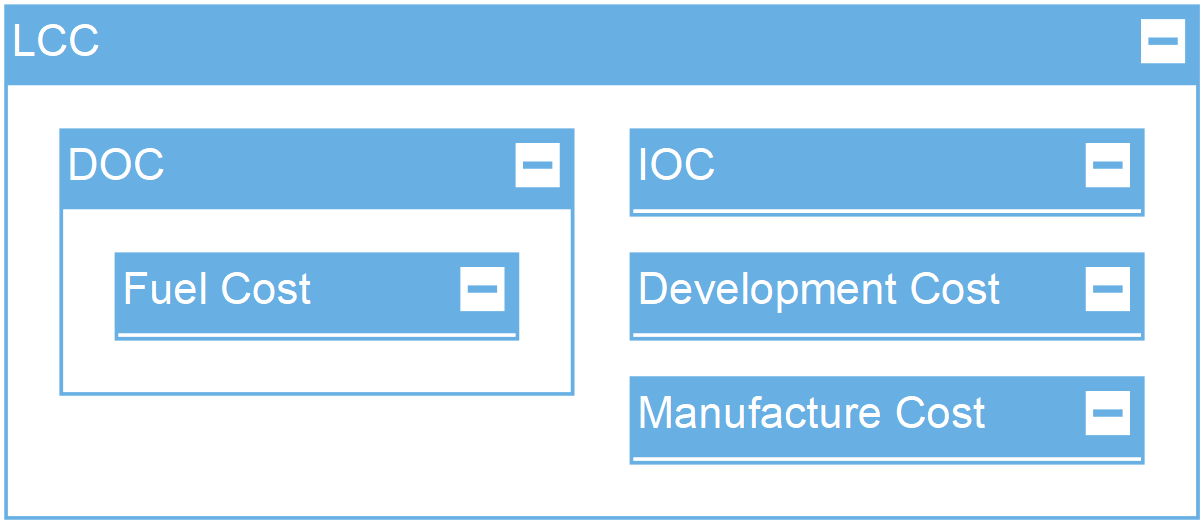
\includegraphics[width=0.8\textwidth]{./media3/image1.png}
	\caption{经济性指标之间的关系}
	\label{fig:ecofactors}
\end{figure}

以飞机的燃油消耗改善为优化目标为例,在飞机的优化设计中,该优化设计未必使得飞机其他方面的经济性指标达到最优,这些指标包括飞机的直接使用成本,制造成本等,如图\ref{fig:ecofactors}所示。而对飞机的LCC进行优化则能够兼顾飞机的使用经济性与产业经济性,但是无法计算飞机设计方案所能够带来的收益。

\subsection{商用飞机价值驱动设计}

商用飞机的主要价值体现在完成乘客和货物的运输过程中,为航空公司带来盈利。在充分竞争和相对平衡的市场条件下,航空运输价格和航空公司的运营成本基本匹配,市场条件的变化导致航空公司利润率的波动,进而反映到飞机制造商在飞机价格和飞机经济性指标的要求。

飞机的价值在财务账目上体现为账面价值,在二手交易市场上体现为相对真实的市场价值,大部分飞机价值评估参考IASTA定义的飞机标准价值。商用飞机的市场价值在其使用周期内会发生变化,

\subsection{价值模型定义}

作为一项更加综合的评估指标,价值模型可以是多样的、多层次的,和多视角的,最基本的价值模型是一个评分模型,该模型以产品的属性为输入。确定一架飞机的价值的属性应该主要包括六个方面:飞机经济性,飞机性能,安全性,环保性,乘客满意度以及飞机维修性等。

在飞机设计初始阶段,飞机的安全性以及飞机的维修性的评估信息相对缺乏,因此,在目前的价值模型计算中,并没有将飞机的这两个属性并没有包含在飞机的价值模型中。 

在产品全寿命周期内,由于价值主体的转移,以及不同价值主体不同的商业模式和目标,价值模型可以是多样的、多层次的,和多视角的。最基本的价值模型可以视为一个评分模型,该模型以产品的属性为输入,采用一系列方法来定义特定市场环境下产品的价值。

不同类型的飞机对其评价指标体系和评价方法是有差异的,对于民航飞机评价来说,其价值属性主要反映在安全性、经济性、舒适性和环保性这四个主要方面,市场竞争性的要求包括六个方面:飞机经济性,飞机性能,安全性,环保性,乘客满意度以及飞机维修性等。

价值驱动设计是一种改进的设计流程,它是多学科综合设计与传统系统工程相结合的方法,使用更灵活的需求定义,优化方法和数学价值模型来取得性能,成本,工程进度等对不同利益相关者的利益影响之间的平衡。相较于传统的系统工程满足要求的设计,价值驱动设计以产品的价值为目标函数,最终是要得到价值最优的设计。价值驱动设计能够探索的设计空间更大,能够得到比传统系统工程更优的解决方案。以价值函数为目标函数的设计,能够得到更加客观的飞机设计方案。

\subsubsection{商用飞机的价值函数定义}\label{valuefunction}
本报告提出的一种典型价值模型函数可以定义为:
\begin{equation}
\label{valuefun}
V(x)=w_1\times DOC(x)+w_2 \times P(x)+w_3 \times N(x)+w_4\times S(x) + w_5 \times E(x)
\end{equation}
式中,$w_i, i=1,...5$为各项指标函数的权重系数,$DOC$代表直接使用成本,$P$代表制造商的利润率或者盈亏平衡点,$N$代表飞机的噪声,$S$代表客户(航空公司或乘客)对飞机的满意度,$E$代表飞机的排放。

尽管在表现形式上相似,价值函数中权重的定义不应简单等同于多目标优化方法中对多个设计目标的加权处理方法。多目标优化方法中的加权处理将多个目标转化为单一目标函数,以便应用常用的数学优化方法,权重系数对优化过程是透明的,不同的目标函数需要进行归一化处理;而价值函数的意义在于体现了决策过程中不同的价值量对决策的影响,其取值对决策者或决策过程是可见的,权重系数的变化对决策结果的影响是可见的。

在飞机设计初始阶段,飞机的安全性以及飞机的维修性的评估信息相对缺乏,因此,在目前的价值模型计算中,并没有将飞机的环保性和舒适性这两个属性并没有包含在目前飞机的价值模型中。 多目标决策的一些方法,例如AHP(Analytic Hierarchy Process)方法,可以用于价值驱动的设计决策过程,一些主要的方法在后续章节进行介绍。


%%%%%%%%%%%%%%%%%%%% Figure/Image No: 2 starts here %%%%%%%%%%%%%%%%%%%%
\begin{figure}[H]
	\centering
		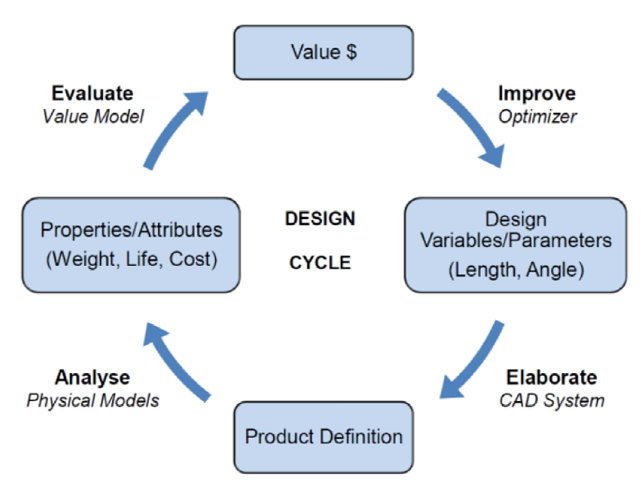
\includegraphics[width=0.8\textwidth]{./media3/image2.png}
		\caption{价值驱动设计方法}
		\label{fig:g32_vdd}
\end{figure}
%%%%%%%%%%%%%%%%%%%% Figure/Image No: 2 Ends here %%%%%%%%%%%%%%%%%%%%

\vspace{\baselineskip}
图\ref{fig:g32_vdd}的设计流程表示价值驱动设计由多次迭代进行,从右侧的设计变量开始,设计团队在设计空间中任意选择一个尝试设计的点。设计变量构成了设计的粗略轮廓。工程师通常使用基于物理的预测建模工具(例如有限元应力 - 应变模型或计算流体动力学)来估计对象的属性。图\ref{fig:g32_vdd}中较低的两个弧为设计从内部参数到产品属性的映射,而左上角的关系则为产品属性到产品价值之间的映射。产品参数与产品的属性是设计团队所关心的,而产品的外在功能和价值是客户所关心的,因此价值驱动设计为产品的内部结构与产品的外在价值搭建了桥梁。在价值驱动设计中,使用目标函数或值模型评估属性,该模型为任何属性集提供标量分数。在每一迭代循环中价值模型都会输出评分,如果在某一次循环中得到的循环优于其他循环,则可以接受该设计成为最优设计。右上角价值驱动设计中的价值模型,是设计迭代中的目标函数。价值驱动设计不是一个优化过程,价值驱动设计并未规定设计人员使用何种设计方法或者优化算法,而是一个允许使用优化的框架。

\subsubsection{剩余价值}
Hollingsworth说明了剩余价值的推导以及剩余价值模型在商用飞机设计中的参数敏感性研究\cite{hollingsworth2011an}。经济学家使用NPV通过贴现未来年度的收益和成本来计算生命周期内的利润或净收益。最大化NPV是最大化利润的计算方法,这是投资决策的共同基础。剩余价值的计算类似于NPV,NPV指未来资金(现金)流入(收入)现值与未来资金(现金)流出(支出)现值的差额。在本文所研究的商用飞机的剩余价值是一种简化的计算模型,剩余价值计算的是飞机制造商,发动机制造商与航空公司的利润总和\cite{collopy1997surplus},这也是剩余价值模型相对于其他经济性评估指标的优点,因为它考虑了飞机设计中多方利益相关方的利益。从另一个层次上来说,剩余价值计算的是整个飞机项目的收益减去成本,剩余价值如图\ref{fig:g33svmodel}所示。


%%%%%%%%%%%%%%%%%%%% Figure/Image No: 4 starts here %%%%%%%%%%%%%%%%%%%%
%\begin{figure}[H]	
%  \begin{subfigmatrix}{2}
%	\subfigure[x]{\includegraphics[width=0.45\textwidth]{./media3/image8.pdf}}
%	\subfigure[x]{\includegraphics[width=0.45\textwidth]{./media3/image9.pdf}}
%  \end{subfigmatrix}
%\end{figure}
%%%%%%%%%%%%%%%%%%%% Figure/Image No: 4 Ends here %%%%%%%%%%%%%%%%%%%%

%%%%%%%%%%%%%%%%%%%% Figure/Image No: 3 starts here %%%%%%%%%%%%%%%%%%%%
\begin{figure}[H]
	\centering
		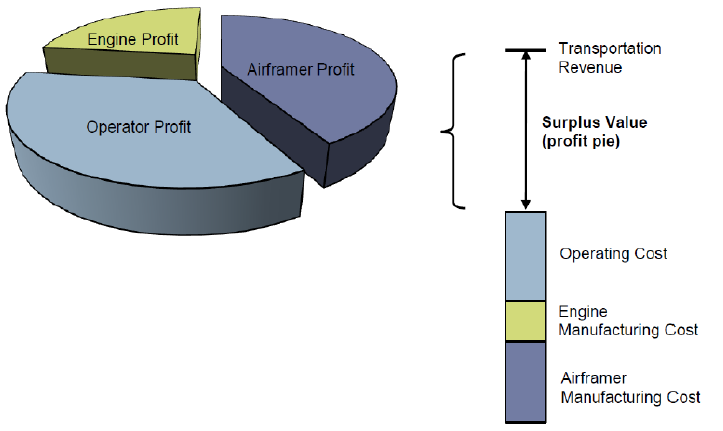
\includegraphics[width=0.8\textwidth]{./media3/image3.png}
		\caption{剩余价值模型}
		\label{fig:g33svmodel}
\end{figure}
%%%%%%%%%%%%%%%%%%%% Figure/Image No: 3 Ends here %%%%%%%%%%%%%%%%%%%%

剩余价值理论表明,企业的最佳发动机设计与实际复杂工业中实际发动机制造商的最佳发动机设计相同\cite{collopy1997surplus}。由于剩余价值考虑了更全面的利益从相关方,并且考虑了成本与收益,因此以上的剩余价值模型在一定程度上反应了航空产业结构的真实情况。剩余价值模型的提出为飞机的设计活动提供了一个很好的经济性判别依据。相比其他传统的基于成本地分析方法,基于DOC的设计方法关注的是航空公司的使用成本,却无法对飞机制造商以及发动机制造商的成本与收益进行考虑。而飞机的LCC只能计算成本,无法对飞机的收益进行考虑。基于剩余价值模型的价值驱动方法同时考虑了飞机所产生的成本与收益,同时兼顾了多方利益相关人的利益。除此之外,价值驱动设计扩大了设计空间,提高了获得最优设计方案的可能性。通过引入剩余价值评价指标,使得飞机的设计决策更加客观理性。因此相比基于成本的方法,基于剩余价值模型的价值驱动设计方法能够兼顾更多的利益相关方,同时考虑了成本与收益,能够得到平衡且综合最优的设计方案。

\subsubsection{剩余价值计算模型}
剩余价值所涉及的利益相关方包括发动机和飞机的净现值,其中收入由销售价格和市场规模以及机票价格共同决定,成本包括飞机的制造成本,研发成本以及航空公司的运营成本。剩余价值模型的建立有多种形式,本研究的剩余价值的计算如下:

\begin{equation}
\label{surplusvalue}
SV={{D}_{p}}\times {{N}_{market}}\times \left[ {{D}_{c}}\times U\times \left( {{R}_{flight}}-{{C}_{flight}} \right)-{{C}_{man}} \right]-{{C}_{dev}}
\end{equation}
式中, $D_{p} $为飞机制造商的折扣系数,$ D_{c}$为航空公司的折扣系数;$ N_{market}$ 为市场规模大小,$U$为飞机的年利用率,$ R_{flight} $是每次运营的收入,$ C_{flight} $是每次飞行的运营成本, $ C_{man} $为飞机的制造成本,$ C_{dev} $ 飞机的研发成本,式中各项成本的单位为美元。

式(\ref{surplusvalue})通过引入贴现来比较不同时期内成本与收益的不同。通过 $ D_{p} $ 来调整计算飞机制造商的净现值(Net Present Value,NPV),通过 $ D_{c} $ 来调整计算航空公司的NPV。 $ D_{p} $ 与 $ D_{c} $ 是分开计算的,因为航空公司的回报周期与飞机制造商或者发动机的产品周期并不相同。对于制造商与航空公司的折扣系数考虑了项目的未来价值以及项目的投资期限,折扣系数的计算如下:

\begin{equation}
\label{discvalue}
Disc=\frac{1}{\sigma }-\frac{1}{\left[ \sigma \times {{\left( 1+\sigma  \right)}^{{{t}_{\Pr oject}}}} \right]}
\end{equation}
式中,$  \sigma  $ 为折扣率, $ t_{Project} $  于制造商来说是投资期限,对于航空公司来说是投资回报周期。

飞机的年平均飞行次数的计算如下:
\begin{equation}
\label{utilization}
U=\frac{{{T}_{YearFlightHours}}}{{{T}_{BlockTime}}}
\end{equation}
式中,${{T}_{BlockTime}}=f\left( Ma,H,W,T,R \right)$,其中,$ T_{YearFlightHours} $ 飞机的年飞行小时数,h。 $ T_{BlockTime} $  为轮挡时间,飞机的轮挡时间是速度,飞机重量,飞机总推力与任务航程的函数,  $ Ma $ 为马赫数,
 $H$  为飞机的飞行高度, $W$ 为飞机的重量,飞机的重量是飞机设计参数x的函数, $w=f \left( x \right)  $ ,kg。$ T $ 为飞机的推力,kn。 $R$ 为任务航程,nm。

每趟航班的盈利 $ R_{flight} $ 的计算与任务航程,飞机的机票价格有关,本模型的机票价格估算采用民航航空公司运输价格改革方案中的机票价格计算方案。此外 $ R_{flight} $ 的计算还与客座率 $  \gamma  $ ,座位数 $ s $ ,货物重量 $ W_{c} $ 以及货物收费 $ p_{c} $ 相关。

飞机的运营成本 $ C_{flight} $ 包括工资,导航费,飞机的餐饮费,机场收费,燃油成本,地面服务费,航空基金与维修费,其中直接使用成本的组成见图2-5。这些成本地计算与飞机的参数有关,这些参数包括设计参数,例如飞机重量,发动机涵道比,航空公司的运营参数 $ X_{A,operation} $ 如机组人员的工资,以及宏观经济环境 $ X_{Ecnonmy} $ 比如航空燃油价格,物价上涨水平等参数相关。采用远程和中短程飞机直接使用成本计算方法进行使用成本的计算,详细的计算方法与参数关系可以参考。

\begin{equation}
\label{operationcost}
{{C}_{flight}}=f\left( X,{{X}_{A,operation}},{{X}_{Ecnonmy}} \right)
\end{equation}

制造商的制造成本 的计算与飞机的设计参数如飞机重量,发动机涵道比,制造商的运营参数  $ X_{M,operation} $  $ X_{M_{Operation}} $ 如劳务费用,制造商设计活动相关参数 $ X_{M,manufacture} $  $ X_{M_{Manufacture}} $ 如材料费用以及宏观经济环境 $ X_{Economy} $ 比如物价上涨水平等参数相关,对 $ C_{man} $ 的计算采用RAND的方法\cite{levenson1972cost},详细的计算方法与参数关系可以参考该报告。

\begin{equation}
\label{manufacturecost}
{{C}_{man}}=f\left( X,{{X}_{M,operation}},{{X}_{M,manufacture}},{{X}_{Economy}} \right)
\end{equation}

制造商的研发成本 $C_{dev} $ 机的设计参数 $ X $ , 制造商的运营参数 $ X_{M,operation} $ 比如劳务费用,制造商设计活动相关参数 $ X_{M,manufacture} $ 如材料费用,实验费用以及宏观经济环境 $ X_{Economy} $ 如物价上涨水平等参数相关。对 $ C_{dev} $ 的计算采用RAND的方法\cite{levenson1972cost},详细的计算方法与参数关系见该报告。

\begin{equation}
\label{randcost}
{{C}_{dev}}=f\left( X,{{X}_{M,operation}},{{X}_{M,manufacture}},{{X}_{Economy}} \right)
\end{equation}

剩余价值这一新的飞机方案评估指标的计算有赖于公式\ref{surplusvalue}每个项目的准确计算,计算每个项目的经验公式计算方法封装于飞机设计程序中。

\subsubsection{剩余价值模型的验证计算}

目前剩余价值尚未在飞机的方案优化中应用,因此需要通过间接的方法对剩余价值指标进行验证计算。剩余价值模型的计算有赖于剩余价值模型中的每一个成本项目的准确计算。这些成本项目准确计算的前提是对飞机相关属性的可靠计算,因为成本的计算需要重量模块,气动模块的计算结果。本研究对飞机设计程序的验证见表2-8,表2-8将飞机设计程序的计算结果与现有机型做了比较,所验证的机型包括窄体客机与远程宽体客机,相关计算结果的误差在允许范围内。在飞机设计程序计算的基础上,需要对剩余价值的计算展开验证,包括直接使用成本,研发成本与制造成本的验证。需要分别对其进行验证计算以保证剩余价值模型计算的可靠性。

\begin{enumerate}
\item 直接使用成本的计算与验证

对于直接使用成本的验证计算采用每公里座位数的DOC作为评价指标,飞机设计程序对每公里座数的直接使用成本相关计算结果如图\ref{fig:g34}所示:

\begin{figure}[H]
	\centering
		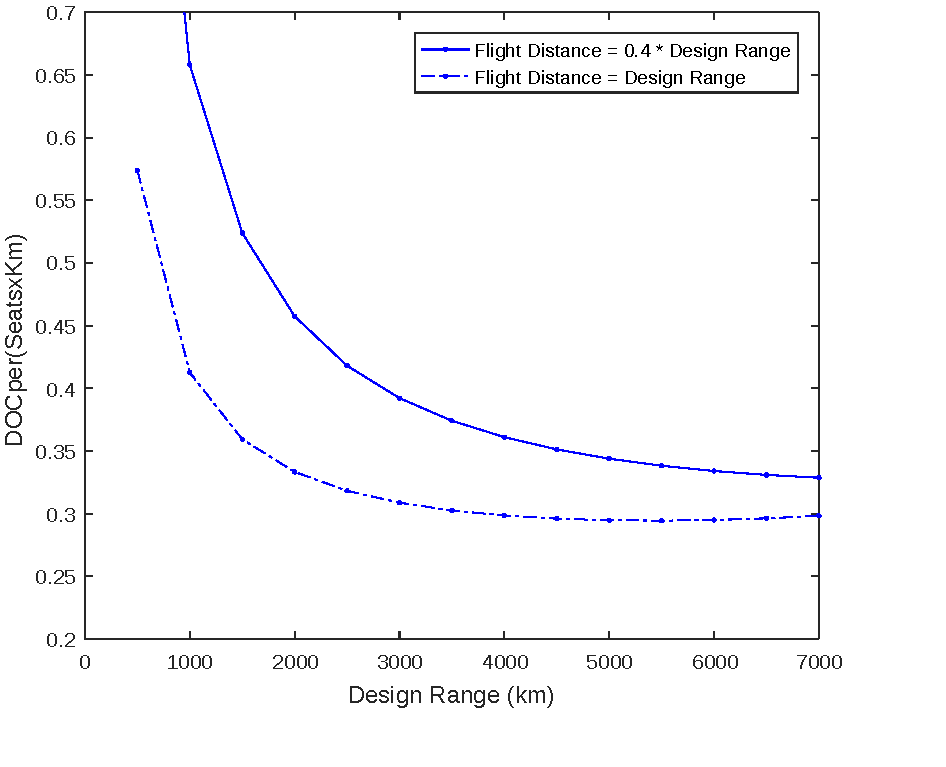
\includegraphics[width=0.8\textwidth]{./media3/image17.pdf}
		\caption{DOC Per (Seats$\ast$Km)}
		\label{fig:g34}
\end{figure}

从图\ref{fig:g34}可以得知,当飞机的设计航程等于实际运行航程,飞机每公里座位数的直接使用成本随着设计航程先快速递减后缓慢增加,当飞机的实际运行里程等于0.4倍设计航程,飞机每公里座位数的直接使用成本下降,在这种情况下,飞机的设计航程为6000km,飞机的实际航程为2400km,飞机每公里座位数的直接使用成本为0.34¥,符合实际情况,该直接使用成本模块的计算结果合理。

\item 研发成本与制造成本的验证计算
\end{enumerate}

在缺乏实际的飞机研发成本与制造成本的详细数据的条件下,本研究采用间接验证的方法,通过对比A320的售价以及文献调研的数据,并与飞机设计程序的计算结果进行验证。

A320 在2019的目录价格为$P_{unit}=1\times 10^8$美元,考虑到飞机制造商对买方做出的折扣,A320的售价约为$5\times 10^7$美元,设定飞机的产量为$420$架, 通过飞机设计程序计算的单机成本进行计算:

\begin{equation}
C_{unit}=C_{man}+\frac{C_{dev}}{Q}=4.51\times 10^7 \$
\end{equation}
式中,$ C_{unit}<P_{unit}$,考虑到飞机制造商对航空公司做出一定折扣,该计算数值在合理的范围内。当A320的实际售价为 $ P_{unit}=5 \times 10^{7} $ $\$$ ,对A320作盈亏平衡分析,如图\ref{fig:Breakeven_analysis_A320}所示。

在图\ref{fig:g35_Breakeven_analysis_A320}中,当飞机的产量为334架,达到盈亏平衡,符合实际情况。此时所计算的单机成本 
$ C_{unit}=P_{unit}=5 \times 10^{7} $ $\$$ 。因此对A320的制造成本与研发成本计算合理。通过验证飞机的直接使用成本,研发成本与制造成本对飞机剩余价值的计算进行间接验证,因此通过飞机设计程序对剩余价值的计算结果合理。

\subsection{剩余价值模型(SV)与DOC的关系}
飞机的直接使用成本是计算剩余价值的组成部分,两者的关系通过公式\ref{svmodel}的简要表示得到如下关系:
\begin{equation}
SV(X)=f(X,X_E, DOC(X,X_E), E(X,X_E))
\label{svmodel}
\end{equation}
式中,$X$为飞机的设计参数,$X_E$为飞机设计所需要考虑的非设计参数,这些参数包括航空公司的运营参数,宏观经济环境,环境参数等,$E(X,X_E)$为计算SV所需要考虑的其他因素以及成本和收益,包括折扣率$D_p$,飞机制造成本$C_{man}$与研发成本$C_dev$等。

在式\ref{svmodel}中,航空公司的直接使用成本是剩余价值模型计算的组成部分,飞机的包括直接使用成本与间接使用成本,直接使用成本即为$DOC(X,X_E)$。因此我们可以看到基于直接使用成本的机翼方案优化的同时,飞机的剩余价值也进行了改善。但是两者又不完全一样,对飞机剩余价值的优化能够兼顾飞机制造商与航空公司,能够兼顾飞机的成本与收益;除此之外对剩余价值的计算考虑了更多的环境因素。

\subsection{价值驱动设计流程}

价值驱动设计是一个以价值函数为目标函数的设计理念。在价值驱动的飞机设计中,整个设计过程应该包括一些主要任务,首先是建立完整的飞机方案设计流程,这一任务在大部分的飞机设计软件或系统中都已经实现,第二项任务是建立飞机的价值模型,第三项任务是将价值模型融入到飞机的设计流程中,并应用综合优化和权衡分析方法开展价值指标的寻优。VDD的这一流程实现面临的主要问题在于大部分现有的飞机设计软件所聚焦的飞机总体参数的寻优是一个相对封闭的系统,并且主要基于经验模型,融入新的模型往往存在一定难度,需要一个开放的体系架构来实现流程的灵活构建和调整。

价值目标是通过建立价值模型所衡量价值的多属性目标函数,它将多属性集合转化为单一维度的数字价值,价值模型的构建对于价值驱动设计的成功至关重要。在飞机经济性设计中,价值模型的构建基础,就是经济性需求的捕获。经济性需求是整个价值驱动设计流程的初始输入 。

\begin{figure}[ht!]
  \centering
  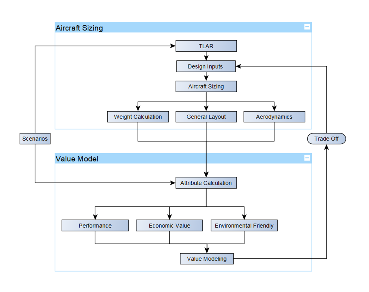
\includegraphics[width=0.8\textwidth]{vdd.eps}\\
  \caption{VDD基本流程}
  \label{fig_vdd}
\end{figure}

任务模块1:飞机总体设计流程:
1.	针对飞机未来的应用场景开展需求分析
2.	对利益相关人的利益进行分析
3.	确定顶层设计要求
4.	确定定义一架飞机的完整技术参数
5.	以顶层设计要求与技术参数作为输入,迭代优化得到更多飞机设计参数

任务模块2:价值模型的建立和分析:
1.	确定定义一架飞机价值的属性
2.	以第一个步骤的参数为输入,计算各个属性值
3.	计算各个属性权重
4.	以第二个步骤的属性计算结果以及第三部的属性权重作为输入,计算飞机的价值函数并得到飞机的价值
5.	根据价值去权衡和优化飞机的技术参数

任务模块3:优化权衡分析
1.	建立分析场景和参数定义
2.	建立场景参数与飞机价值模型之间的关联关系
3.	确定约束条件
4.	确定给定场景下的价值模型


三个模块之间的关系如图\ref{fig_vddflowchart}所示。其中,第一个和第二个模块中的内容给出了较详细的示意,而第三个模块的内容简略代表。愿意在于本项目中第三个模块对应的方法相对而言是比较常用的优化和权衡分析方法,主要依赖于第三方软件,例如MATLAB/Excel的功能支撑来实现。
\begin{figure}[ht!]
  \centering
  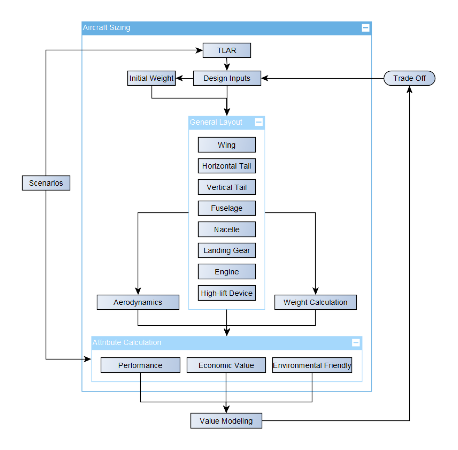
\includegraphics[width=0.8\textwidth]{vddflowchart.eps}\\
  \caption{VDD设计流程的模块关系图}
  \label{fig_vddflowchart}
\end{figure}

在实现了三个基本模块以后,可以开展的任务包括:(1)飞机设计方案的价值分析和评估,包括针对不同的价值函数的参数敏感性分析和关键参数的识别;(2)从飞机全机角度对飞机系统的评估,避免忽略系统之间的相互影响对飞机全机价值的影响;(3)新技术对价值函数的影响分析;(4)不同应用场景下合理的价值函数的选择和分析;(5)价值模型的研究可以对经济性数据工程的工作提供参考,明确需要积累的数据类型和使用目标;(6)有利于完善飞机设计体系,将经济性等竞争性指标更早的介入飞机方案的优化过程,并在飞机项目全寿命周期中应用价值驱动设计的理念和方法推动提高飞机经济性,提高制造商的竞争力。

基于价值驱动的设计方法的进一步发展需要将价值模型和飞机的设计流程与设计工具紧密结合起来,例如,可以将价值模型融入CATIA数模中、项目管理工具中,以及供应商管理环境中。同时,接入典型航空公司的运营数据,应用新的数据分析方法识别对飞机竞争性具有重要影响的技术因素,作为技术规划发展的定量依据。

价值驱动的设计已被用于发动机选择。Cheung\cite{627cheung2012application}通过两个案例研究解释了VDD在航空发动机系统中的应用。盈余价值理论用于提供一个指标,可以通过连续和离散设计变量的变化来权衡组件设计。然而,VDD方法仅适用于一些典型的组件和系统,为了研究子系统和组件的总体影响,仍然需要采用更系统的方法来结合不同级别的设计参数。Cheung给出了一个层次结构,说明了整体飞机性能与其子系统和部件参数之间的关系。飞机系统层次结构如图\ref{fig:aircraftsubsystems}所示,飞机和发动机属性之间的连接如图\ref{fig:aircraftengines}所示。然而,目前的文献只报道了使用价值驱动设计方法对集成飞机/发动机尺寸的很少工作。发动机模型使用线性经验模型构建,Liem\cite{liem2015surrogate}等人在设计中使用了基于发动机性能数据的代理模型和决策专家系统。

\begin{figure}[ht!]
	\centering
		\includegraphics[width=0.8\textwidth]{./eps/aircraft-subsystem-chain.png}
		\caption{飞机系统层次结构}
		\label{fig:aircraftsubsystems}
\end{figure}

\begin{figure}[ht!]
	\centering
		\includegraphics[width=0.8\textwidth]{./eps/aircraft-engine-integration.png}
		\caption{飞机和发动机之间的属性关联}
		\label{fig:aircraftengines}
\end{figure}

商用飞机的价值驱动设计是飞机经济性分析的一种,价值驱动的商用飞机设计流程是复杂的,一个完整的价值模型的建立有赖于飞机设计程序对飞机相关属性的准确计算。因此本文飞机设计方法与程序是飞机价值模型建立的基础,本研究在飞机设计程序的基础上,搭建了价值驱动的商用飞机优化设计框架,该框架如图\ref{fig:g36vdd}所示。

%%%%%%%%%%%%%%%%%%%% Figure/Image No: 15 starts here %%%%%%%%%%%%%%%%%%%%
\begin{figure}[ht!]
	\centering
		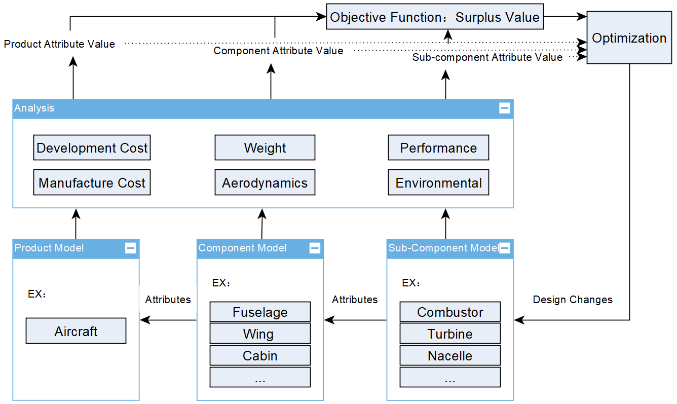
\includegraphics[width=0.8\textwidth]{./media3/image33.png}
		\caption{飞机设计中的价值驱动设计}
		\label{fig:g36vdd}
\end{figure}
%%%%%%%%%%%%%%%%%%%% Figure/Image No: 15 Ends here %%%%%%%%%%%%%%%%%%%%

在图\ref{fig:g36vdd}中,价值驱动的商用飞机优化设计框架的建立过程如下:
\begin{enumerate}
	\item 确定飞机的顶层设计要求;
	\item 确定飞机设计项目的利益相关方,这些利益相关方包括航空公司,旅客,飞机制造商与发动机制造商等;
	\item 确定飞机设计的环境参数,包括设计过程中的环境参数以及飞机实际投入运营的场景参数;
	\item 通过飞机设计参数定义一架完整的飞机设计方案,这些设计参数包括飞机的系统级参数与子系统参数;
	\item 通过飞机设计程序对飞机设计方案进行更多的属性计算,这些属性包括飞机的重量,气动,性能与相关成本估算;
	\item 通过步骤4与步骤5所计算的属性进一步估算飞机的剩余价值;
	\item 设计权衡与优化,迭代和更新飞机的设计参数,得到价值最优的飞机设计方案;
\end{enumerate}

\section{基于场景的方案设计}
飞机的价值受到飞机应用场景的影响,采用基于未来场景的设计有利于飞机制造商进行长远的战略决策。同时为飞机设计团队提供重要的参数参考,使得设计团队更加专注于飞机设计的重要方面,飞机的设计更加具有前瞻性。基于场景设计的优势是该方法可以在所设定的特定场景下进行评估,因此设计工程师可以清楚地了解设计参数在所设定场景中的影响。

飞机的未来应用场景是一组预判值的组合构成的使用换几个,例如十年后的油价,劳动力价值和航空公司航线,机场类型等。在飞机设计价值模型中,飞机的场景参数将为飞机顶层设计要求的确定提供参考与判别依据,同时作为输入计算飞机的属性值,而飞机的属性值是价值模型的输入,因此飞机的场景参数的设定十分重要。以下将飞机的应用场景分为三类,分别是市场环境,运营环境以及技术环境。

以下场景(Scenarios)变量的提取方法,EX:飞机的巡航马赫数是设计变量,在飞机设计定型后不可变;飞机的设计航程不可变,用于飞机设计,但是飞机实际运营有各种航程,因此可以作为场景。

\begin{enumerate}
\item 汇率和关税
\item GDP数据
较低的进口关税有利于飞机制造商降低制造成本,同时较低的出口关税有利于飞机的出口,并提高飞机的全球市场的经济性
\item 飞机燃油价格
民用客机的燃油成本可以占到飞机直接使用成本的$40\%$以上, 因此航空燃油价格对航空公司的运营成本影响是
\item 机场类型
在国内,机场有三种类型。第一类包括首都机场和浦东机场,第二类包括广州机场,虹桥机场,深圳机场,成都机场,昆明机场等。第二类包括杭州,西安 a,重庆,厦门,青岛,海口,长沙,大连,南京,武汉,沉阳,乌鲁木齐,桂林等。每类机场对飞机的经济性产生不同的影响。
\item 年飞行小时数
\item 航线类型 \textemdash 根据目的地的不同,航线分为国内航线和国际航线,对航空公司的运营产生影响。
\end{enumerate}


\subsection{场景的参数定义}

对飞机总体方案的分析与评价需要针对特定的使用环境来考虑,这些因素受到宏观经济环境,航空运输市场条件,航空公司的航线网络特点,特定航线的需求特点等。

1. 宏观经济政策

宏观经济政策可以统计为全球的数据,但是需求预测中一般以国家或地区为单位进行统计,可以以中国和俄罗斯为例做具体的分析,

a)考虑相关国家的GDP增长趋势,人口趋势,因此预测具有长期性,例如目前的预测应该以未来20-30年为框架;
b)可以得到人均GDP,根据IATA的研究得到人均年航班旅行次数,以及总的旅行次数,构成了总得需求量,这得到了每一年的运力需求;
c)世界经济周期对宏观预测的影响体现在经济危机带来需求的延迟;
d)季节性影响在航空公司运力调配上有作用,例如春夏季航班时刻和秋冬季航班时刻安排的变化;
e)国际油价可以考虑,利用其预测数据进行计算,当然国际油价收到许多因素影响;
f)突发事件虽然对航空运输市场会带来影响,事件的发生不具有可预测性,但其影响主要表现在需求发展的时间延迟;
g)税率和汇率有影响,主要是反映出供应链国际化带来的影响,在目前的方案分析中难以考虑进去,同理,政策环境,政府政策等定性描述;

2. 航空公司机队和航线结构

选择两家航空公司,一条航线,例如东航和俄罗斯航空,上海-莫斯科航线,关心如下信息:

a. 其现有宽体机队的机队构成,在这条航线上的航班运力,航班平均上座率(没有数据的话可以采用行业平均值,作为变量)
b. 航段距离,机场条件(构成对宽体飞机的典型设计约束)
c. 票价,可以收集部分数据,作为收入计算

\subsection{飞机顶层设计要求}

飞机顶层设计要求是飞机项目的顶层文档,在整个项目周期内的各个阶段对设计方案的优化和评估起着决定性的作用,确定飞机顶层设计要求需要考虑市场需求,适航标准,技术能力,进度要求,资源需求,以及发展战略等多方面的因素。典型的飞机顶层设计如表\ref{tlar}所示。

\begin{table}[ht!]
\centering
\caption{飞机顶层设计要求}
\small
\begin{tabular}{|p{5.5cm}|p{2.5cm}|p{4cm}|}
\hhline{|===|}
设计指标 &单位 & 典型要求 \\ \hline
座位数(两舱布局,长航程)& & 300 \\ \hline
设计航程 & $nm$ &  5000\\ \hline 
目标任务 & & SHA-MOW  \\ \hline 
设计巡航马赫数/Mach &  &  0.75-0.85 \\ \hline 
起飞场长(MTOW at S-L, ISA+15)  & $m$ & 2800 \\ \hline 
爬升时间(1500ft to ICA at ISA+10)  & $mins$ &  25 \\ \hline 
初始巡航高度(ISA+10)   & $ft$ & 33000-37000  \\ \hline 
最大巡航高度 & $ft$ &  41000 \\ \hline 
进场速度(MLW, S-L, ISA)   & $kts$ CAS & 150 \\ \hline 
着陆场长(MLW, S-L, ISA)  & $ft$ &  2200 \\ \hline 
单发失效高度 &  $ft$ & 分析结果 \\ \hline 
VMO/MMO  & $kts$ CAS / Mach &  TBD / Mcr+0.04\\ \hline 
客舱压力高度 (at 41000ft)  & $ft$  &  6000 \\ \hline 
过站时间 & $mins$ & 参考 \\ \hline 
机场适应性 & &   ICAO E类 \\ \hline 
ACN (Flexible B)  & &  70 \\ \hline 
DOC目标值  & \$/航段  &  参考\\ \hline 
ETOPS/LROPS能力(EIS) &  $mins$ &  180 \\ \hline 
\hhline{|===|}
\end{tabular}
\label{tlar} 
\end{table}

针对几个常用的飞机顶层设计参数的影响可以进行更加具体的分析,以下为针对飞机巡航高度变化、飞机的商载,和飞机的航程对飞机经济性影响的定性分析,定量分析则需要通过使用飞机方案设计工具开展参数的敏感性分析。

\begin{enumerate}
\item[a.]飞机巡航高度
确定喷气运输机的巡航高度应考虑以下几点:按燃油最省原则确定的巡航高度(称为“最佳巡航高度”);满足飞机机动飞行时巡航高度的限制要求;满足高温时发动机推力限制对巡航高度的要求;航程长短和空中交通管制规定对巡航高度的要求。喷气运输机在高空巡航的燃油消耗比低空少,飞行高度愈高,飞行每千米需要的燃油消耗量愈少,但是同时受到空管系统的约束。 

\item[b.]飞机的商载
飞机不同类型客舱的座位数
大多数航空公司的座椅布局分为头等舱、商务舱以及经济舱。尽管经济舱座位数量比例最大,但每座对航空公司收入贡献不大。对于传统航空公司来说,能带来较大利润的则是商务舱。

\item[c.]飞机的航程
飞机的航程越大,所需的载油量也越多,所携带的燃油占有飞机很大的比重,飞机的最大起飞重量也随之增长。飞机带着大量燃油长时间巡航造成飞机的经济性下降。因此飞机的巡航里程影响着飞机的经济性。
\end{enumerate}

%\subsection{基于场景的价值驱动设计}

\section{本章小结}
本章对传统飞机方案设计中的经济性分析与设计展开分析,研究了价值驱动设计的发展以及价值驱动设计在飞机设计中的应用。本研究以前述的飞机设计程序为基础,建立了与飞机设计流程相互耦合的价值驱动飞机设计框架。通过该飞机设计框架能够定量研究飞机设计方案的剩余价值以及环境参数对飞机设计程序的影响。


\chapter{研究方法}

飞机和发动机性能匹配的研究是飞机总体方案设计的重要内容,实现这一目标需要使用飞机的总体设计程序,根据飞机性能的需求确定发动机的设计参数,或者在给定发动机参数的情况下对飞机的参数进行优化设计。在参数优化中,一方面,使用不同的目标函数,对飞机方案设计的结果有很大的影响。本项目对于常用的目标函数进行了分析;另一方面,对于约束条件的考虑是否反映工程应用实际,例如飞行剖面的变化

\section{飞机总体方法实现}

根据飞机不同结构与模块对飞机设计参数以及设计程序进行划分。比如发动机和机翼是飞机的子系统,子系统的属性影响飞机的属性,比如计算全机的重量受到子系统重量的影响;计算全机气动特性受到机翼气动特性的影响。针对飞机的不同子系统,包括机翼,发动机,短舱,平尾,垂尾,起落架,机身,机载设备等子系统,对飞机的设计参数进行划分,这些不同系统的参数共同定义了一架完整的飞机。

本研究通过软件封装飞机的设计公式搭建了如图\ref{fig_vdd_aircraft}所示的完整的飞机设计与优化框架。该软件继承了莫庆华的经济性方法与软件系统,并在此基础上扩展与完善了必要的设计模块。该飞机设计程序以上述不同层级的设计参数作为输入,根据程序所封装的经验公式对飞机的属性进行估算并进一步分析与优化。该飞机设计程序能够评估飞机设计方案对相关成本项目的影响,这些成本项目包括直接使用成本,生产成本,研发成本,全寿命周期成本。除此之外,该设计程序能够计算飞机在一定运行场景下所产生的收益。该飞机设计程序能够对未来的运行环境进行定量分析,并与飞机设计有效耦合。

\begin{figure}[ht!]
  \centering
  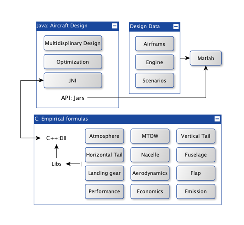
\includegraphics[width=0.8\textwidth]{tool-flowchart.eps}\\
  \caption{多层级的飞机概念设计工具的软件实现}
  \label{fig_tool}
\end{figure}

飞机设计程序的模块与相互关系如图\ref{fig_tool}所示。图中所示的飞机设计程序,分为3个主要部分:第一部分是飞机的底层设计模块,这些模块包含了飞机的子系统部件的多学科计算如飞机的重量与气动,性能与经济性,这些经验公式通过C封装;第二部分是飞机的主程序,飞机的主程序通过JNI(Java Native Interface)接口调用C函数设计方法,通过自有方法将飞机的底层设计模块封装成一个完整的飞机设计程序,进行飞机的多学科设计以及优化;第三部分是飞机的设计参数,这些参数分为飞机的机体参数,发动机参数与全生命周期所涉及的场景参数如飞机制造商的运营参数,宏观经济环境等参数。飞机设计程序通过JAVA层的参数调用接口进行飞机设计方案数据的输入与分析。

整个程序的三个部分的功能模块形成一个多层级的设计系统。不同于类似于PIANO等传统的、完全集成化的飞机概念设计系统,这一架构为设计人员提供了充分的灵活性,可以根据需要替换使用更加准确或者更加高效的分析模块,符合基于模型的系统工程方法的要求。

\subsubsection{飞机方案优化的目标函数}

在飞机方案优化阶段,设计目标和约束条件的确定对于最终的设计结果具有重要的影响,设计约束的来源多样,可以涵盖适航约束、工程约束,和设计约束等。经常用到的一些目标函数可以包括飞机的性能指标和经济性指标,具体可以采用飞机的重量,单机成本,使用成本,飞机的过站时间,以及收益分析等。不同的目标选择对方案的优化结果产生决定性的影响。

\subsubsection{改善飞机经济性的主要手段}
为了改善飞机性能,提高飞机的平均日利用率,民用飞机在交付运营后也需持续设计优化。设计优化可以从以下几个方面降低运营成本:

\begin{enumerate}
\item 通过减重、减阻优化飞机性能和降低运营成本;
\item 通过优化巡航速度和高度降低实际运营油耗;
\item 通过设计优化和完善手册,降低非计划维修成本;
\item 通过优化零部件,降低零部件维修成本;
\item 通过优化运营支持能力,提高飞机签派率;
\item 通过设计优化,解除运营限制项目;
\item 通过设计优化,保障运营可靠性,提升航空公司、乘客信心,消除备机现象
\end{enumerate}

\section{发动机分析模型}

飞机发动机的一体化设计贯穿项目的多个阶段,从总体方案,气动设计,到飞行试验,设计模型同时需要考虑使用维护阶段的需求和因素。总体方案阶段考虑飞机和发动机具有全局影响的总体参数,使用的分析模型强调计算效率,对于常规布局而言,分析模型大多依赖经验数据基础上的拟合模型,辅以部分数值分析模型的使用。对于新的飞机布局,由于缺乏经验数据的支持,数值分析模型的作用大大增加,模型复杂度的提高导致建模的挑战增加,所需要的计算量一般也随之增加,优势在于可以更加准确的分析不同参数和因素的影响。

\subsection{发动机参数定义}

本节给出在方案设计阶段的发动机参数定义,这些参数属于发动机的总体参数,影响飞机的性能,是飞机概念设计阶段开展方案对比和参数优化中涉及的参数,这些参数是开展后续详细设计的基础。


\subsubsection{发动机总体技术参数}

描述发动机特性的总体参数,主要部件分解及各部件的关键参数,将描述发动机特性的总体参数分为主要性能指标参数和设计参数。

\paragraph{主要性能指标}

\begin{enumerate}
\item 推力:在海平面标准大气条件下,发动机静止状态的推力为海平面推力,$N$。
\item 单位推力:发动机的非安装推力与空气质量流量之比。在一定设计推力下,单位推力越大,空气质量流量的设计值越小,相应的发动机尺寸越小,重量也越轻,$N/(kg/s)$。
\item 耗油率:发动机的燃油质量流量与发动机推力之比,表示发动机每工作1小时产生1牛顿推力所消耗的燃油量,即$kg/(N\cdot h)$。民用起飞状态耗油率约为$kg/(N\cdot h)$。
\item 推重比:发动机推重比是在海平面静止条件下发动机最大推力与重力之比,对飞机的主要飞行性能、尺寸和重量有很大影响。客机起飞推重比约为$0.25\sim0.4$。
\item 热效率:热力循环有效功和燃烧室燃油完全燃烧释放热量之比,表示燃油化学能的利用程度。约为$0.25\sim0.4$,取决于发动机飞行条件、循环参数及各部件性能参数。
\item 推进效率:推进功和有效功之比。对于每秒钟流过发动机$1kg$工质气流而言,推进功为单位推力与飞行速度的乘积,而当气流在尾喷管达到完全膨胀时单位推力等于排气速度与进气速度之差,有效功等于进排气动能增量。推进效率随排气速度与进气速度的比值增加而减小。
\item 总效率:发动机所产生的推进功与燃油完全燃烧产生的热能之比,即热效率和推进效率的乘积。总效率随飞行速度或飞行马赫数的增加而增加,随耗油率增加而下降。
\end{enumerate}

在同样飞行速度下,可以用总效率或耗油率来评价发动机的经济性,但在不同飞行速度下只能用总效率来衡量。另外,飞机的经济性不仅仅取决于发动机耗油率,但是对飞机的使用经济性具有重要的影响,在一些长航程航线,燃油成本占据DOC的比例可以达到$40\%$以上,相对中短航程的单通道飞机而言,对燃油经济性的考虑更加重要。

{\centering
  飞机燃油利用率(吨公里/公斤油)=(飞机商载(吨)×航程(公里))/(消耗的燃油(公斤))
}

\paragraph{主要设计参数}
\begin{enumerate}
\item 空气流量\textemdash 每秒流入发动机的空气质量流量,空气流量越大,发动机推力越大,$kg/s$。
\item 总增压比\textemdash 高压压气机出口与发动机进口气流总压之比,总压比影响发动机热力循环有效功和热效率。商用客机一般$25\sim 40$,甚至$40$以上;
\item 涡轮前温度\textemdash 是提高发动机热力循环有效功和热效率的重要参数,提高涡轮前温度可以增大发动机单位推力、减小发动机尺寸、减轻发动机重量和提高推重比。目前已达$1800\sim 2000$K,未来甚至提高到$2000$K以上。
\item 风扇增压比\textemdash 表示了外涵风扇的增压能力。一般约为$1.5\sim 2$。
\item 涵道比\textemdash 目前在役的长航程商用飞机约为$7\sim 12$,下一代将接近$15$。
\item 节流比\textemdash 发动机工作中的最高允许涡轮前温度与地面起飞涡轮前温度之比;
\item 加力燃烧室出口温度\textemdash 接通加力时加力燃烧室出口温度,最大加力状态加力温度取值范围$2000\sim 2150$K
\item 部件性能参数\textemdash 包括各部件效率、总压恢复系数等。
\end{enumerate}

\subsubsection{主要部件分解及各部件的关键参数}

\paragraph{压气机/风扇} 对流入的气体加功增压

\begin{enumerate}
\item 增压比\textemdash 风扇或压气机出口气流总压与进口气流总压之比之比
\item 效率\textemdash 通常用绝热效率表示,达到所需压比的等熵绝热压缩功和实际压缩功之比
\item 单位迎风流量\textemdash 压气机质量流量,和其压气机的最大迎风面积。
\item 喘振裕度\textemdash 发动机的进气口流量变化多少会引发喘振,$\%$。 
\end{enumerate}

\paragraph{涡轮} 将燃烧室出口温度高压燃气的热焓转变为机械功,为风扇、压气机和负载提供带转功率。

\begin{enumerate}
\item 膨胀比\textemdash 涡轮进口总压与出口总压之比,
\item 绝热效率\textemdash 单位工质在一定的涡轮膨胀比下实际产生的膨胀功和等熵绝热条件下产生的理想膨胀功之比
\end{enumerate}

\paragraph{混合器}将涡轮出口高温气流和风扇外涵冷气流进行掺混

\begin{enumerate}
\item 总压恢复系数\textemdash 混合器出口气流总压与进口气流总压的比值
\end{enumerate}

\paragraph{燃烧室和加力燃烧室} 向流入的气体喷入燃油进行燃烧,将燃油的化学能释放出来,使燃气温度提高。
	总压恢复系数:燃烧室出口气流总压和进口总压之比
	燃烧效率:单位质量燃料燃烧时燃气实际获得的热量与燃料低热值之比

\paragraph{尾喷管}使涡轮出口的高温燃气进一步膨胀,以高速排出喷管,将燃气的焓转变为动能。

\begin{enumerate}
\item 总压恢复系数\textemdash 喷管出口气流总压和进口气流总压之比
\item 速度损失系数\textemdash 喷管实际出口气流速度与等熵完全膨胀的理想出口气流速度之比
\item 流量系数\textemdash 尾喷管实际气流流量与理想气流流量之比
\item 角向流系数\textemdash 基本上等于当地出口气流角度的余弦
\item 推力系数\textemdash 实际总推力与理想等熵完全膨胀产生的总推力之比
\end{enumerate}

\subsection{发动机分析模型}

在飞机方案阶段,对不同飞机布局和参数选项,不同涵道比,核心机参数的优化依赖于高效、准确的分析模型,而对分析效率的需求意味着无法直接使用基于数值仿真的模型,需要发展可以在方案阶段使用的半经验模型。常用的半经验模型包括历史数据或型号数据的回归模型,回归模型可以直接采用系统级的参数,也可以通过建立部件级的回归模型,可用的方法有最小二乘估计和高斯回归方法。这类模型可以达到的精度范围在$10\%$左右。

%\subsubsection{发动机重量模型}
%
%
%\subsubsection{发动机油耗模型}
%


\subsubsection{安装特性/推进系统性能}

推进系统由进气道-发动机-喷管三大部件组成,发动机安装的性能参数包括:

\begin{enumerate}
\item 安装推力\textemdash 考虑了装机损失以后的发动机推力,或称有效推力,即气流作用在推进系统内、外表面上作用力的合力,N
\item 安装燃油流量\textemdash 安装后的燃油流量与安装推力之比

\item 安装耗油率(sfc)\textemdash 发动机安装之后的耗油率

\item 进气道的内流特性 \textemdash 进气道的流动品质,可以体现在风扇入口的压力畸变和总压恢复系数表示,进气道总压恢复系数等于进气道出口总压/发动机远前方总压。进气道总压损失越大,进气道总压恢复系数越小。进气道总压恢复系数随飞行马赫数和流量系数的变化关系表示。其中,流量系数定义为远前方未受扰动处气流流管面积与进气道进口面积之比。

\item 进气道的外流特性\textemdash 进气道外流阻力的变化规律,亚声速进气道的外流阻力由附加阻力和进气道外阻力组成。

\item 喷管的内流特性 \textemdash 可用流量系数和推力系数表示。流量系数取决于喷管压比、喷管收敛段的半锥角和喷管收缩比,推力系数为实际总推力与理想等熵完全膨胀产生的总推力之比。

\item 喷管的外流特性 \textemdash 喷管的外流阻力是作用在喷管/后体外表面上的压差阻力,称为喷管/后体阻力,$N$。
\end{enumerate}

\subsubsection{发动机安装性能分析}
发动机安装性能分析涉及的主要工作内容包括,这些性能分析结果影响飞机的性能,进而影响飞机的油耗和经济性指标,是开展经济性权衡分析的关键内容。

\begin{enumerate}
\item 确定进气道捕获面积 \textemdash 选择需要最大捕获面积的飞行条件和发动机最大工作状态为设计点,在此条件下的发动机流量即为进气道的需用流量,再选择喉道设计马赫数,就可以计算出设计点的进气道喉道面积。
\item 确定总压恢复系数和进气道阻力 \textemdash 主要通过两个方面的工作来确定:a) 总压恢复系数在进气道总压恢复系数随飞行马赫数的变化关系图中可以查看; b)流溢阻力特性图:进气道流溢阻力系数增量随飞行马赫数和流量系数的变化关系图
\item 修正进气道总压恢复系数和喷管推力系数对发动机内推力的影响,主要通过三个方面的工作内容来实现:a)用修正因子来修正总压恢复系数对空气流量、燃油流量、喷管压比的影响;b)	查收敛喷管推力系数与喷管压比的关系曲线图,得到安装后的喷管推力系数;c)	重新计算安装后的内推力。
\item 估算喷管/后体尺寸:确定喷管/后体尺寸需要知道喷管/后体尺寸,喷管出口面积可由发动机性能计算程序求得。
\item 确定喷管/后体阻力 \textemdash 由喷管/后体阻力特性图可以查出阻力系数增量。
\item 确定安装性能 \textemdash 安装推力、安装燃油流量和安装耗油率。
\end{enumerate}


\subsubsection{发动机经济性参数及分析方法}
本节以目前长航程商用飞机使用的大涵道比涡扇发动机为研究对象,分析其总体特性参数,经济性的不同评价指标及分析方法,针对飞发一体化设计在飞机总体方案阶段的分析和设计需求。报告内容包括发动机性能指标和顶层参数;发动机部件构成及相关定义参数;飞机发动机一体化安装性能及分析方法。

在参数整理的基础上,需要建立参数间的传递关系,包括飞机顶层设计参数与发动机性能参数的关系,从发动机设计参数到发动机性能指标之间的传递关系依赖于发动机的总体的总体分析程序,以及技术经济性分析方法。

本项研究的基础之一是参考飞机和发动机的一体化概念设计模型,其中包括飞机的概念设计流程和方法,以及发动机的参数分析方法。目前的研究重点是将发动机概念设计中的参数传递关系与飞机顶层设计要求相结合。

发动机的经济性指标包括发动机的价格,维修成本,燃油成本,研发成本,以及发动机的残值等。与发动机经济性有关的特性包括发动机的推海平面推力,油耗水平(SFC),以及发动机的重量。一般来说,同类型的发动机的几何尺寸和重量具有很强的相关性。

\paragraph{发动机价格估算}
单台发动机的价格估算公式( EP,1995年美元计价)如下,该公式将发动机的价格和巡航推力与发动机的油耗进行关联:
\begin{equation}
EP=[0.3857\times \frac{T_{cruise}^{0.88}}{SFC^{2.58}}+0.7286] 
\end{equation}
式中,$T_{cruise}$ 发动机的巡航推力(单位:klbf) ,燃油效率SFC的单位为: lb/hr/lbf。

\paragraph{全寿命周期成本分析}
在全寿命周期成本的概念中,通过产品设计优化,可以实现产品整个寿命周期的成本最小,这一方法体系对于单一成本主体,或者存在最终的单一成本主体的应用场景是有不可替代的意义,这在国防项目中是普遍的情况。但是,对于产品寿命周期中成本主体发生转移的应用场景,其价值主要体现在价值的合理分配上。例如,在平衡的市场条件下,虽然飞机制造商可以通过采用先进的技术来降低飞机的燃油成本,但是增加的研发成本使得其实现盈亏平衡的难度加大。只有当市场愿意接受更高的飞机销售价格的条件下,新技术的应用才能够将制造商的额外的研发成本转移到航空公司身上,最终在直接使用成本中得到平衡。

这一过程中,发动机制造商在降低发动机全寿命周期成本上能够带来的价值与其采用的商业模式存在密切的关系,但是,无论是传统的销售+售后模式,还是不断得到采纳的“Power-by-Hour”模式,低油耗、高可靠性,长寿命是降低发动机全寿命周期成本的三个关键因素,对降低飞机的直接使用成本都是具有积极作用的,能够为航空公司实现更多的价值。

对发动机全寿命周期成本的分析可以借鉴对飞机的全寿命周期成本方法的分析体系,通过对不同阶段的成本进行分析,识别成本驱动变量,建立成本估算关系。全寿命周期成本的框架如\ref{fig-value}所示。

\paragraph{发动机研发和制造成本}
航空发动机的研发和制造成本的估算存在很大的不确定性,市场竞争的压力带来的性能需求使得发动机制造商需要更早开展更多的技术研发,以提高发动机的主要性能参数。成本的估算公式一般将成本和发动机的主要性能参数相关联,通过对类似发动机的历史成本数据进行拟合得到近似的估算方法,这一方法的准确性受到数据准确性的约束,同时由于发动机代际技术的差异带来结果的不确定性。

针对发动机的研发和制造成本的系统研究的公开资料相对较少,比较系统的研究资料为Nelson对航空发动机全寿命周期成本的研究\cite{nelson1977life},该报告发表的时间是1970年代,对发动机全寿命周期成本研究的基本框架仍然具有参考价值,也是后续相关研究的重要参考。成本估算方法在后续的一些研究中得到不断更新,例如Younossi等人对典型对军机发动机项目对成本估算方法进行了分析\cite{younossi2002military},其中聚焦涡轮风扇发动机,采用数据统计方法,考虑发动机参数,制造技术参数等对成本影响的关系史。在该报告的方法基础上,需要结合发动机设计与制造和维护技术的发展,更新设计参数与成本数据的关系。

然而,基于统计分析的方法得到的成本关系式在设计阶段的价值是相对有限的,结合目前CAD技术,物理建模技术,以及过程建模技术,通过对发动机研制过程的分析,以及发动机附件和子系统的进一步分解,可以逐步建立更为详细的参数和单机成本的关系式。

在本项目中发动机研制成本的估算采用已有发动机的历史数据,结合技术发展的合理预测,对所需发动机的研制成本进行拟合估算和修正,以便体现技术发展带来的影响。

\paragraph{发动机维修成本}
对发动机维修成本的影响参数,除了设计参数和发动机可靠性等指标以外,与航班运行有关的因素在下述列表中给出,根据这些因素的分析,可以确定主要的影响参数。

\begin{enumerate}
\item 平均航段长度;
\item 飞机起飞和爬升阶段发动机减推力运行所占的比例;
\item 维修程序的完备性
\item SV的工作范畴,包括对咨询通告的融合政策
\item 与MRO服务提供商的协商议价能力;
\item 发动机送修方案的决策方法
\end{enumerate}

发动机的维修成本随机龄变化,在制造商的商保期内的新机维修成本相对较低,之后随着机龄的增加维修成本稳态上升。达到成熟期后,有可预测的维修成本,老龄以后维修成本再次上升。

计算发动机维修成本可参考AEA的方法,此方法考虑了发动机设计参数的影响,可分为发动机劳务成本和发动机材料成本。其中劳务成本与海平面起飞静推力、涵道比、压气机级数(包括风扇)有关,材料成本与发动机的总压比有关。

\begin{enumerate}
\item 发动机维修劳务成本
与时间有关的发动机劳务成本(美元/飞行小时):
\begin{equation}
L_t=0.21\times R\times C1\times C3\times(1+T)^{0.4}	
\label{engine_dmc_time}
\end{equation}
式中,$R$为工时费(美元/工时),$C1=1.27-0.2B^{0.2}$,$C3=0.032N_C+k$,$T$为海平面起飞静推力;$B$为涵道比;$N_C$为压气机级数(包括风扇);$k$为涡扇发动机轴数的函数(对应单轴,双轴和三轴布局,分别取$k=0.5,0.57, 0.64$)。
与飞机起降次数有关的发动机维修劳务成本(美元/起落次数,\$/cycle)为:
\begin{equation}
L_c=1.3L_t	
\end{equation}

\item 发动机材料成本
与时间有关的发动机材料成本(美元/飞行小时)
\begin{equation}
M_t=2.56(1+T)^{0.8}\times  C1\times (C2+C3)	
\end{equation}
式中,$C2=0.4(OAPR/20)^{1.3}+0.4$,$OAPR$为发动机总压比。与飞机起降次数有关的发动机成本(美元/起落次数)
\begin{equation}
M_{tc}=1.3M_t	
\label{engine_dmc_mat}
\end{equation}

\end{enumerate}

综上,可以得到发动机维修成本可综合如式\ref{engine_dmc},单位为“美元/轮挡时间”:
\begin{equation}
EMC=(N_e(L_t+M_t)(tf+1.3))/(tf+0.25)   
\label{engine_dmc}	
\end{equation} 
式中,$N_e$为每架飞机的发动机数;$t$为轮挡时间(小时);$tf$为空中时间(飞行小时),$tf=(t-0.25)$。

可靠性影响发动机部件的寿命,进而影响发动机的经济性,包括维修本身的成本以及停飞造成的收入损失。目前通常以空中停车率、提前换发率、正点率及平均故障间隔时间MTBF作为衡量发动机可靠性的指标。对发动机制造厂商来说,准确的估算和提高发动机的可靠性可以有效改善发动机的经济性,提高其市场竞争力。

\begin{enumerate}
\item 空中停车率(In Flight Shutdown)指每1000飞行小时中,由于发动机故障造成发动机空中停车的次数。
\item 提前换发率(Unscheduled Engine Removal)指在每1000飞行小时中,由于发动机故障造成未到翻修寿命就提前拆换发动机的次数。
\item 正点率(Departure Reliability)指每100个定期航班中,正点起飞(航班时刻15分钟以内)的航班次数。
\item 延误/取消率为每100个定期航班中,由于发动机原因不能正点开航而造成的延误(延误时间大于15min 才算延误)或取消航班的次数。正点率=1-(延误/取消率)
\item 返修率(Shop Visit Rate)指每100飞行小时,由发动机原因造成的返修次数。
\item 平均故障间隔时间(Mean Time Between Failures)是指对于可维修的产品,产品在两次相邻故障间的平均工作时间。
\end{enumerate}

\section{单选发动机和多选的价值分析}

民用飞机经济性是民用飞机省钱盈利能力的表征。从主制造商的角度而言,民用飞机经济性目标主要由两点构成,一是要更加经济地设计飞机;其次是设计经济性好的飞机。更经济地设计飞机,确定了项目成本基线,保证在项目资源能力范围内实现项目,可以防止亏空,有力保证项目成功;设计经济性好的飞机,降低飞机的使用成本,增强飞机在航线上的盈利能力,使航空公司愿意运营该型号的飞机,则是民用飞机商业成功的重要因素。

飞机/发动机尺寸是降低生产和运营成本的关键。飞机工程计师应与发动机工程师保持持续沟通,以保证良好的飞机性能。由于新发动机循环的开发有时必须与先进机身的开发同时进行,因此有时必须在最终的飞机配置得到明确定义之前进行初始发动机参数调整。在实际启动任何新飞机项目之前,需要了解关键技术和设计因素对未来发动机和机身的潜在影响和益处。

然而,这种组合参数可能并不总是发生,即飞机和发动机是分开设计的。这可能由于多种原因而发生,例如,由于市场需求和/或交付计划的限制,或者发动机公司,飞机制造商试图将现有发动机的修改版本安装到新飞机上可能会尝试在多个飞机项目中使用相同的核心引擎。后一种情况可以在商用飞机项目中常见。然而,许多研究人员已经证明,集成的尺寸调整过程可以提供进一步优化的解决方案。

选择发动机通常有两种可能的情况。一种是为飞机提供特定类型的发动机,另一种是同时提供两种或两种以上发动机选择。这两种情况自然具有其自身的技术,经济和性能优势及风险。不同发动机的推力,燃料消耗,重量和维护特性通常是不同的。不同发动机的工具,备件和培训成本也存在差异。同时选择两种发动机使航空公司可以选择他们偏好的发动机,这通常是航空公司已经运行的发动机,从而降低了运营成本。当只为飞机提供一种发动机时,制造商可以节省设计,工程和认证成本,但市场份额可能会受到影响,因为喜欢其他种类发动机的航空公司可能就不愿意引进这架飞机。但另一方面,具有唯一发动机选项飞机的剩余价值可以得到保护。此外,作为发动机制造商,为了保持其作为唯一供应商的地位,他们更愿意花时间和投资用于发动机的研制,这可以为飞机提供更好的服务。

但单选发动机的风险相对较大。例如,当年洛克希德生产L-1011 TriStar时,他们只有一个发动机选项——劳斯莱斯RB211。而RR发动机没有及时交付,尽管TriStar的设计时间表非常接近其竞争对手,由于发动机研制的延迟,道格拉斯的设计提前一年比洛克希德上市,这也是最终导致该种飞机最终消亡的一个重要原因。因此,具有多个发动机选项可以降低新飞机交付的风险。 此外,发动机制造商之间的竞争可以为航空公司提供更多的讨价还价机会,也具有降低购置费用的潜力。


价值驱动的设计已被用于发动机选择。 Cheung\cite{627cheung2012application}通过两个案例研究解释了VDD在航空发动机系统中的应用。盈余价值理论用于提供一个指标,可以通过连续和离散设计变量的变化来权衡组件设计。然而,VDD方法仅适用于一些典型的组件和系统,为了研究子系统和组件的总体影响,仍然需要采用更系统的方法来结合不同级别的设计参数。Cheung给出了一个层次结构,说明了整体飞机性能与其子系统和部件参数之间的关系。飞机系统层次结构如\ref{fig_chain}所示,飞机和发动机属性之间的连接如图\ref{fig_integration}所示。然而,目前的文献只报道了使用价值驱动设计方法对集成飞机/发动机尺寸的很少工作。发动机模型使用线性经验模型构建,Liem\cite{liem2015surrogate}等人在设计中使用了基于引擎性能数据的代理模型和决策专家系统。

\begin{figure}[ht!]
  \centering
  \includegraphics[width=0.8\textwidth]{aircraft-subsystem-chain.png}\\
  \caption{飞机系统层次结构}
  \label{fig_chain}
\end{figure}

在文献中,价值函数有许多不同的定义。价值评估需要一个直观而有意义的价值函数,该函数支持在备选方案之间进行直接比较。数学价值模型用于表示所有已确定的涉众价值(客户、业务、社会)及其交互,在单个度量中,将项目的需求传达给设计团队的每个成员。随后,VDD方法确保优化单个数学函数中表示的所有利益相关方的价值。由Isaksson提出的概念设计分析模型使用了一个相对价值指标\cite{1297monceaux2014overview},可以看作是描述设计价值或总体客户满意度水平的百分比量表。在最近的文献中,存在更多基于经济的模型,其利用剩余价值作为设计评估的目标函数和基于效用理论的模型来解决客户需求冲突。

本项研究中采用的方法是将发动机的特征参数模型与飞机的总体设计程序实现紧耦合,在没有考虑发动机内在设计逻辑的情况下,可以得到不同发动机总体参数对所关心的价值函数的影响。

\begin{figure}[ht!]
  \centering
  \includegraphics[width=0.8\textwidth]{aircraft-engine-integration.png}\\
  \caption{飞机和发动机之间的属性关联}
  \label{fig_integration}
\end{figure}


\chapter{研究结果及分析}

\section{基于价值驱动方法的飞机设计方案优化与评估}

本节介绍价值驱动设计方法在飞机方案评估中的应用,应用的方向为飞机方案设计的经济性优化。本节将分别以直接使用成本与剩余价值为单目标函数,分别对机翼设计方案以及飞机设计方案进行单目标优化,对比以不同的经济性指标为目标函数的优化结果的不同,并探索直接使用成本与剩余价值之间的关系。由于直接使用成本与剩余价值关注的方面不同,直接使用成本计算的是航空公司的使用经济性,剩余价值计算的是产业经济性,本研究将通过兼顾直接使用成本与剩余价值,建立多目标优化方案,对商用飞机设计方案进行多目标优化。

\subsection{使用的优化算法}

在工程应用领域,特别是多学科设计领域,针对优化方法的研究是开展高效率的优化设计的重要工具,但不是本项目的研究重点。本项目根据文献调研结果和课题组长期的研究经验,主要选用两种优化方法:一是粒子群优化方法,主要用于单目标优化问题的求解;二是用于多目标优化问题的NSGAII方法。两种方法的有效性得到多方验证。
\begin{enumerate}
\item \textbf{粒子群优化算法}

本研究采用带非线性限制条件的粒子群优化算法,采用粒子群优化算法的优点是该优化算法容易找到全局最优解\cite{wang2018particle}。粒子群优化算法是一种进化优化技术,该算法的粒子只有位置和速度两个属性。每个粒子在搜索空间中单独寻优,并记为当前个体的极值,并将个体机制与整体的粒子群极值进行共享和对比,其中最优的个体极值为当前的全局最优解,所有粒子根据当前的最优解调整自己的速度和位置进行更新。

\item \textbf{NSGA-II多目标优化算法}
\end{enumerate}

多目标优化问题是由多个目标函数与等式约束和不等式约束组成。多目标优化模型描述如下:

\begin{equation}
Min F(\textbf{x})=[f_1(\textbf{x}), f_2(\textbf{x}),\cdot, f_m(\textbf{x})]^T
\end{equation}
s.t.
\begin{equation}
g_i(\textbf{x})\le0, i=1,2,\cdot, p
\end{equation}
其中$\textbf{x}={(x_1,x_2,\cdot, x_n)}^T$ 是欧式空间的$n$维设计变量,上述的目标函数,约束函数与设计变量构成了多目标优化的三要素,满足所有约束条件的一组设计变量称为可行解,而优化中的所有可行解构成了可行域。设S为多目标优化的可行域,$\textbf{f}(x)$为多目标优化的向量目标函数,若$\textbf{f}(\textbf{x})\le\textbf{f}(\textbf{x}^-)$ ,$\forall \textbf{x}\in S$,则$\textbf{x}^- $称为多目标优化问题的非劣解,即Pareto最优解集。多目标优化问题的非劣解一般不只一个,所有非劣质构成非劣解集。在多目标优化问题中,往往不存在一个解使得所有目标函数达到最优,一般一个目标函数的改善以另外一个目标函数的损失为代价。在存在多个Pareto最优解的情况下,所有的Pareto解被认为是同等重要的,因此多目标优化的任务是找到一组尽可能不同的并且接近pareto最优域的解集。

%%%%%%%%%%%%%%%%%%%% Figure/Image No: 4 starts here %%%%%%%%%%%%%%%%%%%
\begin{figure}[ht!]
	\centering
		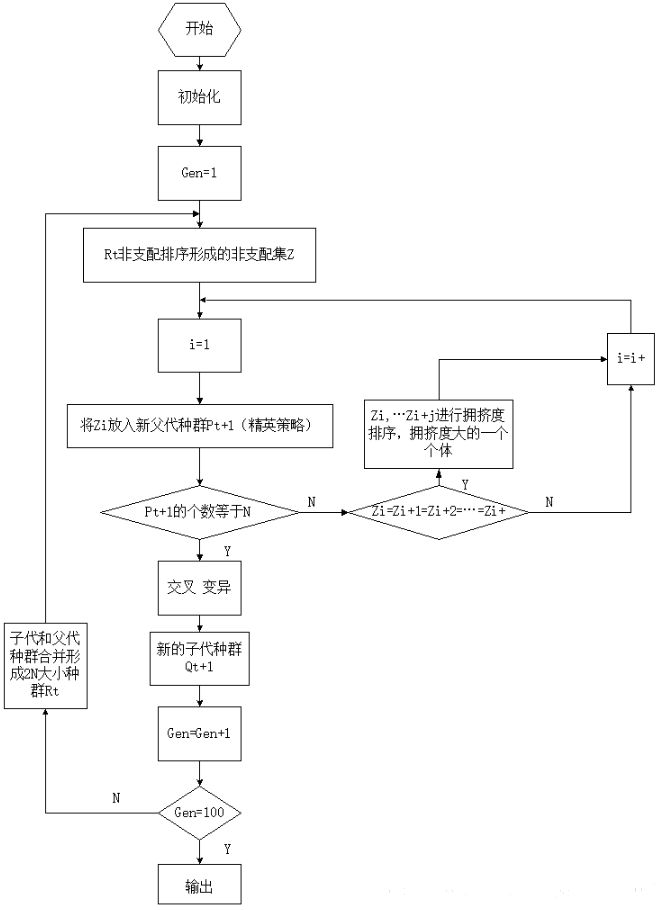
\includegraphics[width=3.35in,height=4.62in]{./media4/image7.png}
		\caption{NSGA算法流程}
		\label{fig:g41_NSGA}
\end{figure}

%%%%%%%%%%%%%%%%%%%% Figure/Image No: 4 Ends here %%%%%%%%%%%%%%%%%%%%

本研究将采用NSGA-II(Non-Dominated Sorting Genetic Algorithm)进行相关设计的优化,NSGA-II是一种解决多目标优化问题的多目标遗传算法。NSGA-II的流程如图\ref{fig:g41_NSGA}所示。

\subsection{机翼设计方案的优化}
\subsubsection{问题描述}
本研究对传统布局的商用飞机展开研究,以186座位数的窄体客机为研究对象,飞机的外形布局为常规布局,采用翼吊式双发布局,飞机的其他设计参数,商业载荷,航程与性能与A320-200类似,所安装的发动机为CFM56-5A1。飞机的设计航程为2700nm,飞机的任务航程为从天津机场到晋江机场,1080nm。采用的本研究所搭建的飞机设计框架进行机翼方案设计的优化和分析。

\begin{enumerate}
\item \textbf{飞机设计要求}

根据市场需求和技术发展确定合理有效的飞机顶层设计指标对项目的技术指标,实施进度,和商业前景具有关键性的影响。制定飞机的顶层设计指标不是一项简单的任务,也并非完全受到市场驱动,其本身应该称为飞机总体方案迭代流程的一环以及结果,以确保其在具有竞争力的同时具备技术和经济上的可行性。典型的飞机设计指标如表\ref{tlar}所示。

%%%%%%%%%%%%%%%%%%%%% Table No: 1 starts here %%%%%%%%%%%%%%%%%%%%
%\begin{table}
%\centering
%\caption{飞机设计方案总体参数指标}
%\begin{tabular}{|p{5cm}|p{6cm}|}
%\hline \hline
%参数	& 名义值  \\ \hline
%Passenger Capacity 	& [2-cl LR]	180  \\ \hline
%Design Range [nm]		& 1000 – 3500  \\ \hline
%Study Mission		& TSN-JJN  \\ \hline
%Design Cruise Speed 	& Mach	0.7 – 0.8  \\ \hline
%Take-Off Field Length [MTOW at S-L, ISA+15, m]		& 2600  \\ \hline
%Time to Climb [1500ft to ICA at ISA+10, mins]		&  25  \\ \hline
%Initial Cruise Altitude [ISA+10, ft]		& 33000 – 37000  \\ \hline
%Maximum Cruise Altitude [ft]		&  41000  \\ \hline
%Approach speed [MLW, S-L, ISA, kts CAS]		&  150  \\ \hline
%Landing Field Length [MLW, S-L, ISA, m]		& 1600  \\ \hline
%VMO / MMO,kts CAS / Mach		& TBD / Mcr+0.04  \\ \hline
%Airport compatibility limits-		& ICAO Code ‘C’  \\ \hline
%DOC [RMB/trip or RMB/(seat·km)]		& Reference  \\ \hline
%\hline
%\end{tabular}
%\label{tab-tlar}
%\end{table}

对机翼的6个设计参数进行优化设计,这6个参数分别为机翼参考面积S,展弦比A,梢根比,厚度比t/c以及四分之一弦长后略角以及飞机的设计巡航马赫数Ma。机翼的设计参数以及其上下限如表\ref{wing-pars}所示。

\begin{table}
\centering
\caption{机翼的一些典型参数}
\begin{tabular}{|p{2.4cm}|p{2.4cm}|p{2.4cm}|p{2.4cm}|}
\hhline{|====|}
Parameters	& Lower bounds	& Upper bounds	& Initial Design \\ \hline
S[m$^2$]	& 105	& 135	& 122.4 \\ \hline
A	&7.5	& 11	& 9.4 \\ \hline
$\lambda$ 	& 0.2	& 0.3	& 0.24 \\ \hline
$\Lambda$ [deg] &	20	& 30	&25 \\ \hline
t/c	& 0.1	& 0.18	& 0.14 \\ \hline
Ma	& 0.7	& 0.8	& 0.79 \\ 
\hhline{|====|}
\end{tabular}
\label{wing-pars}
\end{table}

%%%%%%%%%%%%%%%%%%%% Table No: 2 ends here %%%%%%%%%%%%%%%%%%%%

\item \textbf{约束条件}
\end{enumerate}

在机翼的优化设计中需要添加约束条件使得该设计方案更加合理,这些约束条件包括飞机的起飞降落性能,飞机的爬升率,静稳定裕度,飞机重心的前后限以及机翼展长的限制。约束条件的具体设置如表\ref{wing-cons}所示。

\begin{table}
\centering
\caption{机翼的一些设计约束}
\begin{tabular}{|p{7cm}|p{3cm}|}
\hhline{|==|}
Constraints		& Value \\ \hline
Span[m] &	<=40\\ \hline
Forward C.G location [\% MAC]	& >=	12 \\ \hline
Backward C.G location [\% MAC]	& <=	32 \\ \hline
Climb rate	& >=	0.024 \\ \hline
Takeoff field length[m]	& <=	2500 \\ \hline
Landing field length[m]	& <=	1700 \\ 
\hhline{|==|}
\end{tabular}
\label{wing-cons}
\end{table}

\subsubsection{基于DOC的机翼设计单目标优化}
剩余价值与DOC分别以不同的层面对飞机的经济性做出评估,剩余价值关注的是整个航空产业的盈利能力,飞机的剩余价值模型能够兼顾飞机制造商,发动机制造商与航空公司的利益,DOC则强调的是航空公司的使用成本,两者考虑的利益相关方不同。

航空公司的直接使用成本为传统飞机经济性评价指标,是衡量飞机使用经济性的一项关键指标,是航空公司关注的参数。本研究以DOC为优化目标函数,对机翼设计方案进行优化。以DOC为目标函数的机翼方案优化流程如图\ref{fig:vdd-process}所示。

\begin{figure}[ht!]
	\centering
		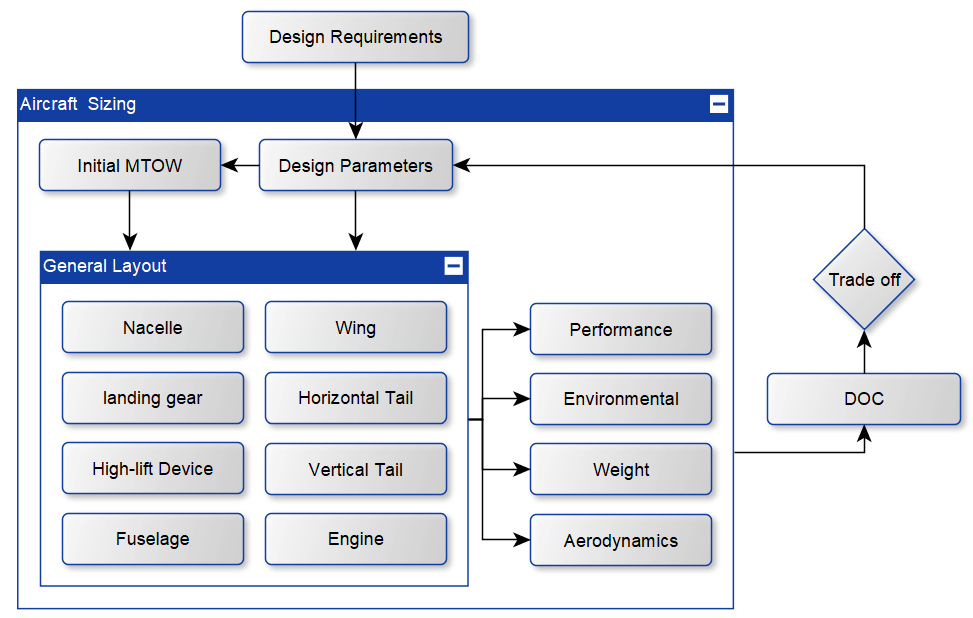
\includegraphics[width=0.8\textwidth]{./media4/image10.png}
		\caption{价值驱动的DOC的优化流程}
		\label{fig:vdd-process}
	
\end{figure}

以DOC为目标函数的优化过程如图\ref{fig:vdd-process}所示,图中DOC的优化流程的基础为飞机设计的方法与程序,通过本研究的飞机设计程序进行计算,最终得到飞机的性能,环保,重量以及飞机的气动特性,通过上述的计算结果进一步计算飞机的直接使用成本。机翼的方案设计参数以及飞机设计程序计算得到的这些属性共同影响飞机的直接使用成本,并对机翼的设计参数进行基于DOC的优化。以DOC为优化目标的问题的描述如下:

\begin{equation}
Min: F_{DOC}(\textbf{x})=\frac{DOC(\textbf{x})-DOC_{baseline}}{DOC_{baseline}} \times 100\%
\end{equation}
约束条件:$g(\textbf{x})\le g_0(\textbf{x})$,
其中\textbf{x}是机翼的设计参数,$DOC_{Baseline}$是基准机型的直接使用成本,目标函数${{F}_{DOC}}(\textbf{x})$表示机翼优化方案相对基准机型的改善百分比。机翼的设计参数的上下界见表\ref{wing-pars},约束条件见表\ref{wing-cons},以飞机设计方法为基础,通过飞机设计程序以及带非线性限制条件的PSO优化算法对机翼进行方案优化设计。PSO的群大小设置为400,最大迭代次数为1000,基于${{F}_{DOC}}(\textbf{x})$目标函数的设计方案优化过程如图\ref{fig:g43PSO}所示。

\begin{figure}[ht!]
	\centering
	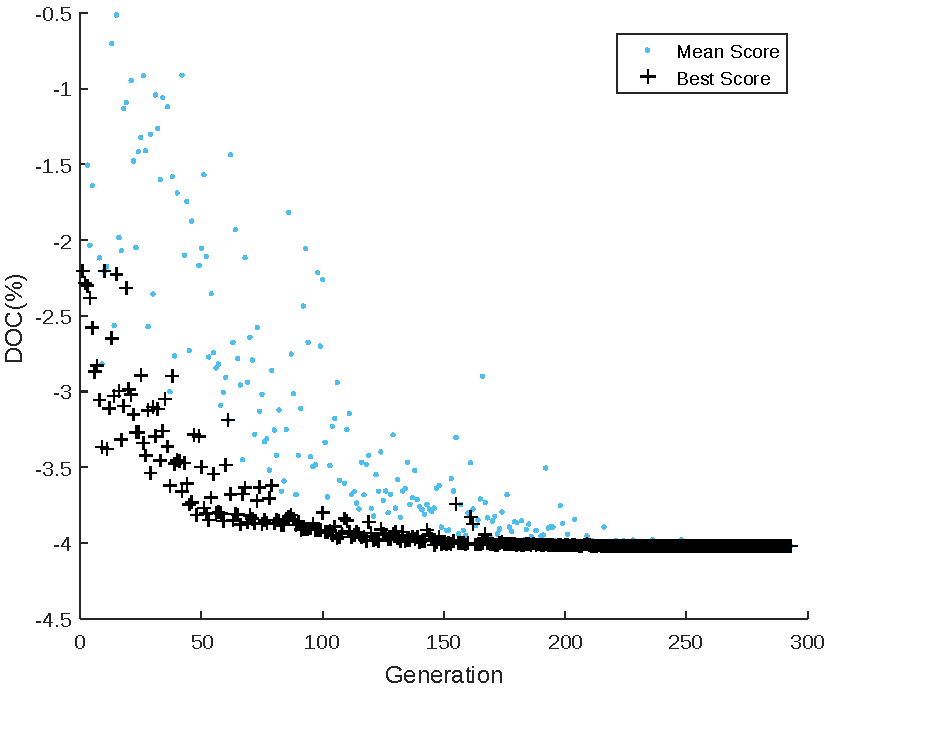
\includegraphics[width=0.75\textwidth]{./media4/image19.pdf}
	\caption{目标函数为$F_{DOC} \left( x \right) $的优化过程}
	\label{fig:g43PSO}
\end{figure}

从图\ref{fig:g43PSO}可以看到基于${{F}_{DOC}}(\textbf{x})$目标函数的设计方案优化过程收敛,设计的结果如表\ref{wing-results-doc}所示。

\begin{table}[ht!]
\centering
\caption{优化结果(目标函数为DOC)}
\begin{tabular}{|p{4.8cm}|p{2.3cm}|p{4.5cm}|}
\hhline{|===|}
Parameters	& DOC results &	 DOC for Initial Design \\ \hline
S [m$^2$]	& 121.19	& 122 \\ \hline
A	& 9.89	& 9.4 \\ \hline
$\lambda$	& 0.20	& 0.24 \\ \hline
$\Lambda$ [deg]	 &25.00	 & 25\\ \hline
t/c	 & 0.12	 & 0.14\\ \hline
Ma	& 0.8	& 0.78\\ \hline
Takeoff field length [m]	& 1867.5	& 1913\\ \hline
Landing field length [m]	& 1600	& 1524\\ \hline
b [m]	& 31.3	& 34\\ \hline 
C.G. [$\%$ MAC]	& 25.64	& 25.16\\ \hline
Climb rate	& 0.058	& 0.0541 \\ \hhline{|===|}
\hline
\end{tabular}
\label{wing-results-doc}
\end{table}

从表\ref{wing-results-doc}可以看到,基于DOC的优化方案,飞机的机翼参考面积相比基准机型略有下降,飞机的展弦比上升,梢根比下降,机翼的厚度比下降,飞机的设计马赫数上升。飞机升阻比的提升能够降低飞机的燃油消耗,提升飞机的使用经济性。从该表还可以看到,该优化设计方案的相关约束条件,包括飞机的起飞场长与降落场长,机翼展长,飞机的重心范围以及爬升梯度在合理的范围之内,因此该设计方案合理。

\subsubsection{基于SV的机翼设计单目标优化}
剩余价值作为一个更加全面的飞机经济性评价指标,考虑了更多的利益相关人方,对飞机的经济性分析覆盖了整个飞机的整个生命周期,基于剩余价值的优化问题描述如下:
\begin{equation}
Min F(\textbf{x})=[f_1(\textbf{x}), f_2(\textbf{x}),\cdot, f_m(\textbf{x})]^T
\end{equation}
s.t.
\begin{equation}
g_i(\textbf{x})\le0, i=1,2,\cdot, p
\end{equation}
式中,\textbf{x}是机翼的设计参数,$S{{V}_{Baseline}}$是基准机型的直接使用成本,目标函数${{F}_{SV}}(x)
$表示机翼优化方案相对基准机型的改善百分比。机翼的设计参数应该满足飞机设计的限制条件 $ \sigma  $ ,限制条件的设置见表\ref{wing-cons},$ lb $ 与 $ ub $ 分别为设计参数的上下界,见表\ref{wing-pars}。以飞机设计方法为基础,通过飞机设计程序以及带非线性限制条件的PSO优化算法对机翼进行方案优化设计。PSO的群大小设置为400,最大迭代次数为1000,基于${{F}_{SV}}(x)$目标函数的设计方案优化过程如图\ref{sv-results}所示。

\begin{figure}[ht!]
	\centering
	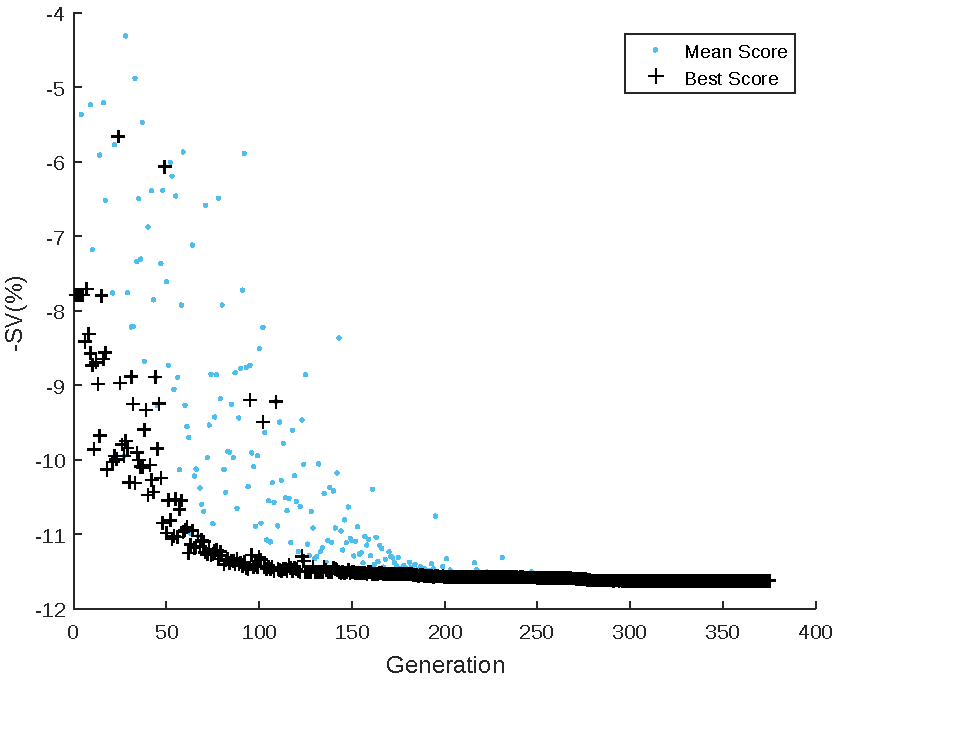
\includegraphics[width=0.8\textwidth]{./media4/image27.pdf}
	\caption{目标函数为 $ F_{SV} \left( x \right) $的优化过程}
	\label{sv-results}
\end{figure}
从图\ref{sv-results}可以看到基于${{F}_{SV}}(x)$目标函数的设计方案优化过程收敛,方案优化的结果如表\ref{wing-results-sv}所示。

\begin{table}[ht!]
\centering
\caption{优化结果(目标函数为SV)}
\begin{tabular}{|p{4.8cm}|p{2.3cm}|p{4.5cm}|}
\hhline{|===|}
Parameters	& SV results & SV for Initial Design \\ \hline
S [m$^2$]	& 112.09	& 122 \\ \hline
A	& 9.72	& 9.4 \\ \hline
$\lambda$	& 0.20	 & 0.24 \\ \hline
$\Lambda$ [deg]	 & 25.00	& 25 \\ \hline
t/c	& 0.10	& 0.14 \\ \hline
Ma	& 0.80	& 0.78 \\ \hline
Takeoff field length [m]	& 2000	& 1913 \\ \hline
Landing field length [m]	& 1600	& 1524 \\ \hline
b [m]	& 33	& 34 \\ \hline
C.G. [\% MAC]	& 24.25	& 25.16 \\ \hline
Climb rate	& 0.057	& 0.0541 \\ \hhline{|===|}
\end{tabular}
\label{wing-results-sv}
\end{table}

从表\ref{wing-results-sv}可以看到,基于 $ F_{SV} \left( x \right)  $ 的优化设计方案,飞机的机翼面积下降,飞机的展弦比相比初始设计方案略有提升。机翼的梢根比下降,飞机的厚度比下降,飞机的巡航马赫数提升。根据表\ref{wing-results-sv},展弦比的增加有助于提升飞机的剩余价值;而出现上述优化结果的原因是该受到起飞与着陆场长约束条件的限制。相关的限制条件包括飞机的起飞场长与降落场长,飞机的机翼展长,飞机的重心范围以及飞机的爬升梯度满足相关的设计约束,设计方案合理。

\subsubsection{两种机翼优化设计方案的对比}
对比两种不同的经济性指标可以看到优化结果并不完全相同。分别以飞机的剩余价值为目标函数进行优化的结果与基准设计方案的对比如图\ref{wing-comp}所示:

\begin{figure}[ht!]
	\centering
	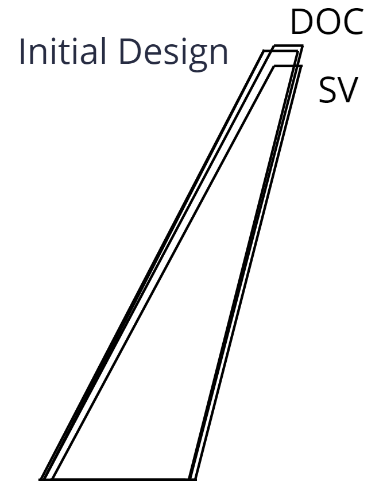
\includegraphics[width=0.5\textwidth]{./media4/image28.png}
	\caption{不同目标函数得到的优化设计结果}
	\label{wing-comp}	
\end{figure}

探索两种不同的优化设计方案的相关属性,这些属性包括飞机的剩余价值SV,航空公司的直接使用成本DOC,飞机制造商的研发成本以及制造成本,飞机的燃油消耗,飞机的空机重量以及飞机的MTOW,如图\ref{wing-comp2}所示:

\begin{figure}[ht!]
	\centering
	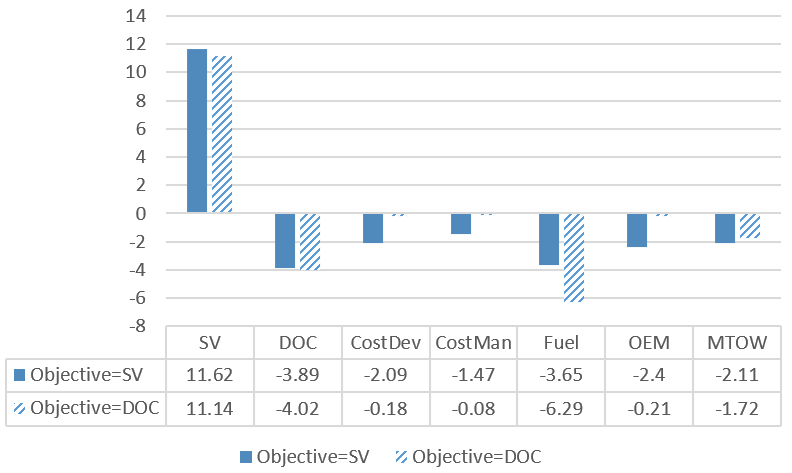
\includegraphics[width=5.06in,height=3.02in]{./media4/image31.png}
	\caption{两种优化方案与基准设计方案的对比}
	\label{wing-comp2}
\end{figure}

从图\ref{wing-comp2}可以看到,以 $F_{SV} \left( x \right)  $ 为目标函数进行机翼的设计方案优化,飞机相对基准设计方案的剩余价值提升了11.62$\%$ ,飞机的直接使用成本下降了3.89$\%$ ,飞机的研发成本下降了2.09$\%$ ,飞机的制造成本下降了$1.47\%$ ,飞机的燃油消耗改善了$3.65\%$ 。除此之外,飞机的空机重量下降了$2.4\%$ ,飞机的MTOW下降了$2.11\%$ 。飞机的空机重量的下降以及飞机最大起飞重量的下降会对飞机的研发成本与制造成本进行改善。从图\ref{wing-comp2}可以看到,相比基于 $ F_{DOC} \left( x \right)  $ 的优化设计方案, $ F_{SV} \left( x \right)  $ 优化方案的优化过程能够对研发成本与制造成本进行计算,通过对空机重量的优化对研发成本与制造成本进行优化。因此 $ F_{SV} \left( x \right)  $ 优化设计方案则兼顾了制造商与航空公司等多方利益相关人的利益,不仅对飞机的使用经济性进行改善,同时也提升了飞机的产业经济性。

\subsubsection{多目标总体优化设计方案}
在对机翼进行单目标优化时可以看到两种不同的优化方案多关注的方面并不相同,基于剩余价值模型的机翼方案优化能够兼顾多方利益相关人的利益,能够同时考虑成本与收益。而基于DOC的机翼方案优化则更加强调飞机的使用经济性,只能对航空公司的成本进行计算。两者优化方案的优化结果并不相同,但是都显示出对飞机经济性的盖上。在机翼设计中,直接使用成本的优化需要和剩余价值的优化进行综合考虑,才能够实现飞机使用经济性和航空产业经济性的协调,提高飞机的综合经济性,这对新型的飞机制造商有为重要。通过多目标优化算法对飞机的剩余价值与直接使用成本进行优化,能够得到更加具有平衡和综合最优的机翼设计方案。

在图\ref{pareto-doc-sv}中,基于剩余价值的单目标优化与基于直接使用成本的单目标优化分别位于Pareto非劣解集合的两端。在pareto非劣解集合的这些设计方案能够同时兼顾飞机的使用经济性与飞机的产业经济性,得到平衡与综合最优的设计方案,提升飞机设计方案的经济性。
\begin{figure}[ht!]
	\centering
	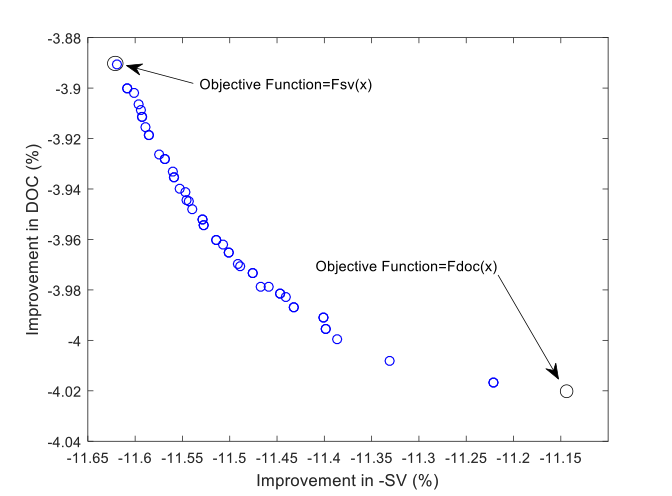
\includegraphics[width=0.8\textwidth]{./media4/pareto-doc-sv.png}
	\caption{Pareto非劣解集合}
	\label{pareto-doc-sv}
\end{figure}

\subsection{飞机设计方案的参数优化}
\subsubsection{问题描述}
本研究对传统布局的商用飞机展开研究,以186座位数的窄体客机为研究对象,飞机的外形布局为常规布局,采用翼吊式双发布局,飞机的其他设计参数,商业载荷,航程与性能与A320-200类似,所安装的发动机为CFM56-5A1。飞机的设计航程为2700nm,飞机的任务航程为从天津机场到晋江机场,1080nm。简化的飞机设计流程如图3-6所示,采用的本研究所搭建的飞机设计框架进行方案设计的优化和分析。

在上一节针对机翼参数的优化设计的基础上,增加了4个总体参数,对飞机的10个设计参数进行优化设计,这10个参数分别为机翼参考面积$S$,展弦比$A$,梢根比$\lambda$ ,厚度比$t/c$,四分之一弦长后略角$\Lambda$ ,飞机的设计巡航马赫数$Ma$,飞机的机身长度${{L}_{F}}$,发动机推力$T$,发动机涵道比${{R}_{bypass}}$以及航程R,飞机的设计参数以及其上下限如表\ref{aircraft-pars}所示。

\begin{table}
\centering
\caption{飞机总体方案的一些典型参数}
\begin{tabular}{|p{2.4cm}|p{2.4cm}|p{2.4cm}|p{2.4cm}|}
\hhline{|====|}
Parameters	& Lower bounds	& Upper bounds	& Initial Design \\ \hline
S[m$^2$]	& 105	& 135	& 122.4 \\ \hline
A	&7.5	& 11	& 9.4 \\ \hline
$\lambda$ 	& 0.2	& 0.3	& 0.24 \\ \hline
$\Lambda$ [deg] &	20	& 30	&25 \\ \hline
$t/c$	& 0.1	& 0.18	& 0.14 \\ \hline
$Ma$	& 0.7	& 0.8	& 0.79 \\ \hline
$L_F$ [m] & 32	&  43	& 37.57 \\ \hline
$T$  & 20000	& 30000	& 25000 \\ \hline
$BPR$ & 4	& 8  &  6 \\ \hline
$R$  & 3500	&  6500	&  5000 \\ \hhline{|====|}
\end{tabular}
\label{aircraft-pars}
\end{table}

\subsubsection{基于DOC / (Seats$\ast$ Km)的单目标优化}
本研究还采用了每公里座位数的直接使用成本DOC / (Seats$\ast$ Km)为指标对飞机方案进行优化设计。DOC / (Seats$\ast$ Km)的计算如下:

\begin{equation}
DO{{C}_{per}}(x)\text{=}\frac{DOC(x)}{Seats\times Km} 
\end{equation}

以DOC/(Seats$\ast$ Km)为优化目标的问题中,目标函数的定义如下:

\begin{equation}
Min: F(\textbf{x})=\frac{DOC_{per}-DOC_{perBaseline}}{DOC_{perBaseline}} \times 100\%
\end{equation}
式中,$\textbf{x}$是飞机的设计参数,$DOC_{perBaseline}$是基准机型的每公里座位数的直接使用成本,目标函数$F(x)$表示飞机优化方案相对基准机型的改善百分比。飞机的设计参数应该满足飞机设计的限制条件 $  \sigma  $ ,约束条件的设置与机翼优化问题中约束条件相同,设计参数的上下界见表\ref{aircraft-pars}。以飞机设计方法为基础,通过飞机设计程序以及带非线性限制条件的PSO优化算法对飞机进行方案优化设计。PSO的群大小设置为600,最大迭代次数为1000,基于$F(x)$目标函数的设计方案优化过程如图\ref{fig:g48_aircraftdoc}所示。

\begin{figure}[H]
	\centering
		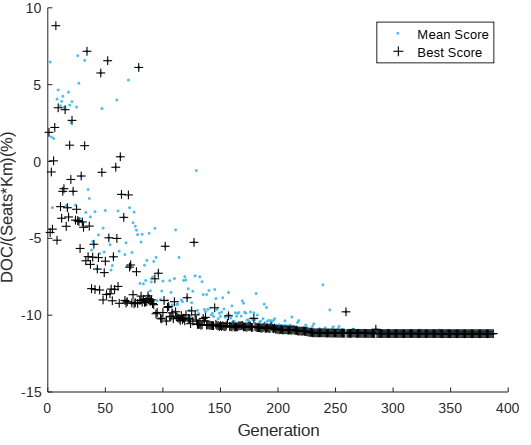
\includegraphics[width=0.8\textwidth]{./media4/aircraft-doc.png}
		\caption{目标函数为 $ F \left( x \right)  $ 的飞机方案参数优化过程}
		\label{fig:g48_aircraftdoc}
\end{figure}
从图\ref{fig:g48_aircraftdoc}可以看到基于$F(x)$目标函数的设计方案优化过程收敛,设计的结果如表\ref{aircraft-results}所示。

从表\ref{aircraft-results}可以看到,基于DOC/(Seats$\ast$ Km)的优化方案,飞机的机翼参考面积相比基准机型略有上升,飞机的展弦比上升,梢根比下降,机翼的厚度比下降,飞机的设计马赫数上升。飞机设计马赫数的提升以及飞机升阻比的提升能够降低飞机的燃油消耗,提升飞机的使用经济性。该优化设计方案中,起飞场长的计算达到了约束边界,因此上述的优化结果是优化边界的解集中对DOC/(Seats$\ast$ Km)最优的解。从表\ref{aircraft-results}可以看到,该优化设计方案的相关约束条件,包括飞机的起飞场长与降落场长,机翼展长,飞机的重心范围以及爬升梯度在合理的范围之内,因此该设计方案合理。

\begin{table}[ht!]
\centering
\caption{优化结果(目标函数为DOC/(Seats$\ast$ Km)}
\small
\begin{tabular}{|p{3.5cm}|p{3.3cm}|p{4cm}|}
\hhline{|===|}
Parameters	& DOC results &	 DOC for Initial Design \\ \hline
S [m$^2$]	& 126.94	& 122 \\ \hline
A	& 9.65	& 9.4 \\ \hline
$\lambda$	& 0.20	& 0.24 \\ \hline
$\Lambda$ [deg]	 &25.00	 & 25\\ \hline
t/c	 & 0.12	 & 0.14\\ \hline
Ma	& 0.8	& 0.78\\ \hline
$L_F$ [m] & 41.15	& 37.57 \\ \hline
$T$  & 29517	& 25000 \\ \hline
$BPR$ & 8  &  6 \\ \hline
$R$  & 5887.5	&  5000 \\ \hline
Takeoff field length [m]	& 2100	&1913\\ \hline
Landing field length [m]	& 1587	& 1524\\ \hline
b [m]	& 34.93	& 34\\ \hline
C.G. [\% MAC]	& 25.30 & 25.16\\ \hline
Climb rate	& 0.0566	& 0.0541 \\ \hhline{|===|}
\end{tabular}
\label{aircraft-results}
\end{table}

\subsubsection{基于SV的单目标优化}
以剩余价值为目标函数的飞机方案价值驱动设计的优化问题得到的结果。从表\ref{aircraft-results-sv}可以看到,基于 $ F_{SV} \left( x \right)  $ 的优化设计方案,飞机的机翼面积下降,飞机的展弦比相比初始设计方案略有提升,机翼的梢根比下降,飞机的厚度比下降,飞机的巡航马赫数提升,飞机的机身长度增加,座位数随之增加,发动机的推力增加,发动机的涵道比增加,航程略有缩短。相关的限制条件包括飞机的起飞场长与降落场长,飞机的机翼展长,飞机的重心范围以及飞机的爬升梯度满足相关的设计约束,设计方案合理。

\begin{table}
\centering
\caption{优化结果(目标函数为SV)}
\small
\begin{tabular}{|p{4.5cm}|p{2.8cm}|p{4cm}|}
\hhline{|===|}
Parameters	& SV results &	 SV for Initial Design \\ \hline
S [m$^2$]	& 123.86	& 122 \\ \hline
A	& 9.86	& 9.4 \\ \hline
$\lambda$	& 0.20	& 0.24 \\ \hline
$\Lambda$ [deg]	 &25.00	 & 25\\ \hline
t/c	 & 0.18	 & 0.14\\ \hline
Ma	& 0.80	& 0.78\\ \hline
$L_F$ [m] & 43	& 37.57 \\ \hline
$T$  & 26169.8	& 25000 \\ \hline
$BPR$ & 8  &  6 \\ \hline
$R$  & 4181	&  5000 \\ \hline
Takeoff field length [m]	& 2000	&1913\\ \hline
Landing field length [m]	& 1600	& 1524\\ \hline
b [m]	& 34.95	& 34\\ \hline
C.G. [\% MAC]	& 28.22 & 25.16\\ \hline
Climb rate	& 0.0556	& 0.0541 \\ \hhline{|===|}
\end{tabular}
\label{aircraft-results-sv}
\end{table}

\subsubsection{两种优化设计方案的对比}
探索两种不同的优化设计方案的相关属性,这些属性包括飞机的剩余价值SV,航空公司的直接使用成本$DO{{C}_{per}}$,飞机制造商的研发成本以及制造成本,飞机的燃油消耗,飞机的空机重量以及飞机的MTOW,如图\ref{fig:aircraft-doc-sv}所示:

\begin{figure}[ht!]
  \centering
  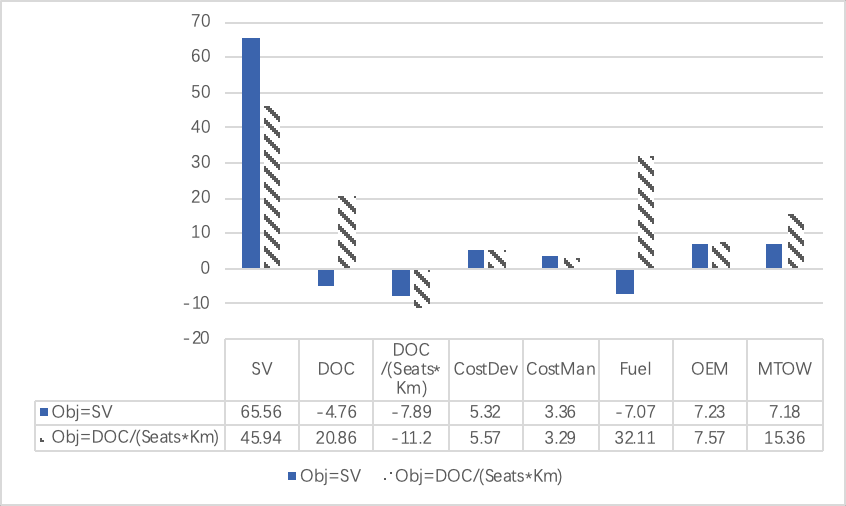
\includegraphics[width=0.8\textwidth]{./media4/aircraft-doc-sv.png}
  \caption{两种优化方案与基准设计方案的对比}
  \label{fig:aircraft-doc-sv}
\end{figure}

从图\ref{fig:aircraft-doc-sv}可以看到,以 $ F_{SV} \left( x \right)  $ 为目标函数进行飞机的设计方案优化,飞机相对基准设计方案的剩余价值提升了$65.56\%$ ,飞机的直接使用成本下降了$4.76\%$ ,而每公里座位数的直接使用成本则下降了$7.89\%$ 。由于飞机空机重量的提升,飞机的研发成本增加了$5.32\%$ ,飞机的制造成本增加了$3.36\%$ ,飞机的燃油消耗改善了$7.07\%$ 。从g该图还可以看到,相比基于 $ F_{perDOC} \left( x \right)  $ 的优化设计方案, $ F_{SV} \left( x \right)  $ 优化方案对飞机的空机重量以及最大起飞重量的增幅更小,对制造商的研发成本的改进幅度也比基于 $ F_{perDOC} \left( x \right)  $ 的优化设计方案大, $ F_{SV} \left( x \right)  $ 优化设计方案则兼顾了制造商与航空公司等多方利益相关人的利益,不仅对飞机的使用经济性进行改善,同时也提升了飞机的产业经济性。

\subsubsection{多目标优化设计方案}
在对飞机进行单目标优化时可以看到两种不同的优化方案多关注的方面并不相同,基于剩余价值模型的机翼方案优化能够兼顾多方利益相关人的利益,能够同时考虑成本与收益。而基于DOC/(Seats$\ast$ Km)的机翼方案优化则更加强调飞机的使用经济性,只能对航空公司的成本进行计算。在飞机设计中,直接使用成本的优化需要和剩余价值的优化进行综合考虑,才能够实现飞机使用经济性和航空产业经济性的协调。多目标问题的结果如图\ref{fig:aircraft-pareto}所示。

\begin{figure}[htp]
  \centering
  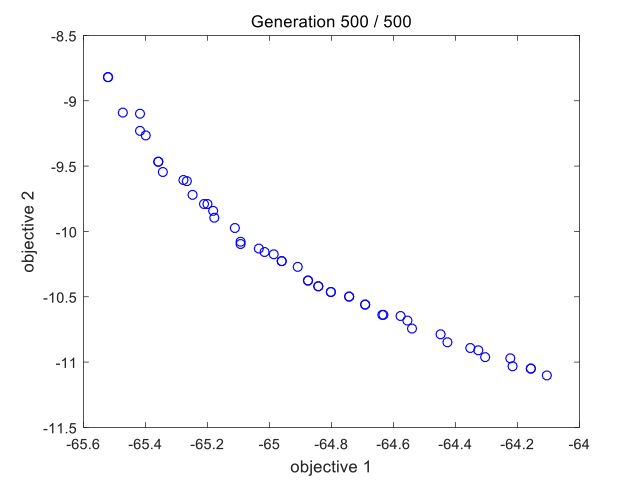
\includegraphics[width=0.8\textwidth]{./media4/aircraft-pareto.png}
  \caption{飞机方案参数的Pareto 非劣解集合}
  \label{fig:aircraft-pareto}
\end{figure}

在图\ref{fig:aircraft-pareto}中,在pareto非劣解集合的这些设计方案能够同时兼顾飞机的使用经济性与飞机的产业经济性,得到平衡与综合最优的设计方案,提升飞机设计方案的经济性。

\subsection{设计参数的敏感性分析}
针对剩余价值与直接使用成本的飞机设计方案单目标优化显示了两种设计方案的不同。飞机不同的设计参数对飞机经济性的影响是不同的,本研究对飞机的部分设计参数做了相关属性的敏感性分析,探索不同飞机设计参数的经济性敏感性不同。在飞机的设计参数中,不同的设计参数对飞机经济性的影响的方式与路径不同,比如飞机的机翼面积的改变,将会对飞机的重量,气动与性能产生影响,并最终影响飞机的经济性。

\begin{enumerate}
\item \textbf{机翼参考面积改变对飞机设计的影响}

机翼参考面积的改变对飞机设计产生多方面的影响,包括飞机的重量特性,气动特性与性能,进而影响飞机的经济性。机翼参数的改变对飞机设计的影响如图\ref{fig:wingarea}所示。

\begin{figure}[htp]
  \centering
  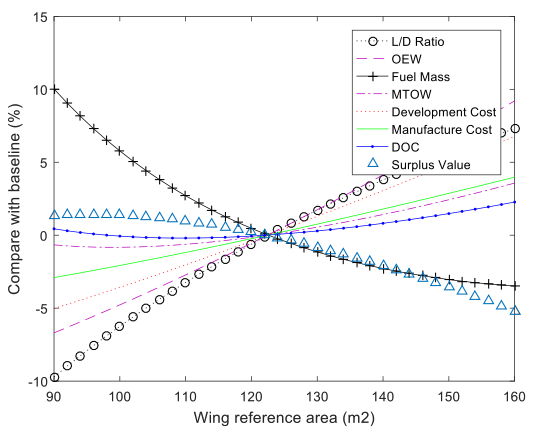
\includegraphics[width=0.8\textwidth]{./media4/wingarea.png}
  \caption{机翼参考面积的相关敏感性分析}
  \label{fig:wingarea}
\end{figure}

图\ref{fig:wingarea}显示机翼参考面积的改变对飞机设计的影响。机翼参考面积增加使得飞机的升阻比增加,飞机的气动性改善,进而使得飞机的燃油消耗下降。由于机翼的升阻比增加,飞机的空机重量增加,进而导致飞机的研发成本与制造成本增加。飞机气动性能的改善在一定程度降低了燃油消耗,然而飞机重量的增加使得飞机的重量增加,并增加了燃油消耗。飞机的直接使用成本同时受到两者的影响,随着机翼参考面积的增加,先下降后提升,而飞机的剩余价值与直接使用成本的变化呈相反趋势,先缓慢上升后下降。

\item \textbf{飞机展弦比改变对飞机设计的影响}

飞机的展弦比是机翼的重要参数,展弦比的该改变将影响飞机的重量,气动与性能,进而影响飞机的经济性。展弦比对飞机设计的影响如图\ref{fig:aspectratio}所示。

\begin{figure}[htp]
  \centering
  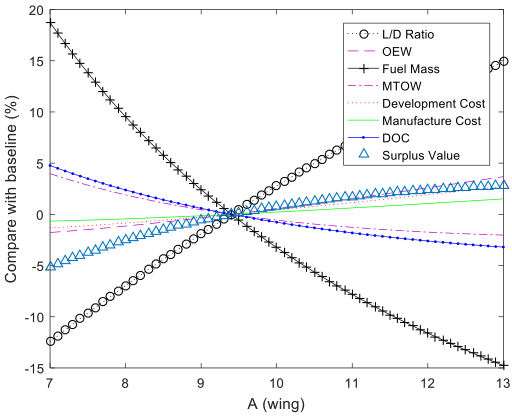
\includegraphics[width=0.7\textwidth]{./media4/aspectratio.png}
  \caption{机翼展弦比的敏感性分析}
  \label{fig:aspectratio}
\end{figure}

图\ref{fig:aspectratio}中,飞机的升阻比随着展弦比的提升而增加,并且飞机的最大起飞重量随着展弦比的提升而下降,这两者的改善使得飞机的燃油消耗下降。除此之外,飞机的展弦比的增加使得飞机的空机重量上升,飞机的研发成本与制造成本增加。相比飞机的重量因素以及飞机的制造成本与使用成本,飞机展弦比的改变对飞机的气动特性影响更大,进而对飞机的燃油带来的改善大于飞机重量增加对燃油消耗带来的负面影响。燃油消耗的改善使得飞机的使用经济性带来了极大的提升,飞机直接使用成本下降的同时,飞机的剩余价值上升。

\item \textbf{梢根比改变对飞机设计的影响}

飞机的梢根比会对飞机的性能,气动特性,重量产生影响,这些飞机设计属性相互影响,进而对飞机的经济性产生影响。飞机的梢根比对飞机设计的影响如图\ref{fig:taperratio}所示。

\begin{figure}[htp]
  \centering
  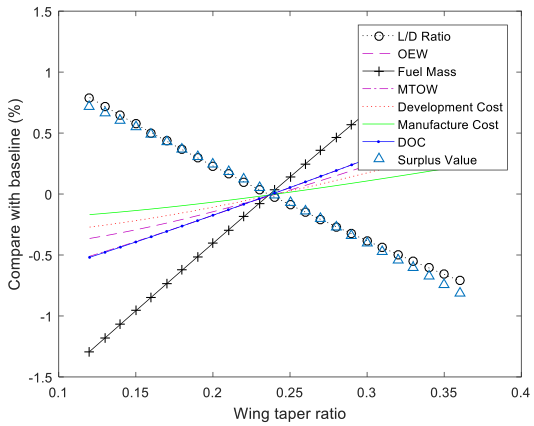
\includegraphics[width=0.8\textwidth]{./media4/taperratio.png}
  \caption{机翼梢根比的敏感性分析}
  \label{fig:taperratio}
\end{figure}
从图\ref{fig:taperratio}可以看到,随着机翼梢根比的增加,飞机的重量增加,升阻比下降,在两者的共同影响下,飞机的研发成本与制造成本增加,燃油消耗增加,这些因素导致飞机的使用成本增加以及剩余价值的下降。

\item \textbf{设计马赫数的影响}

飞机的设计马赫数会对飞机的气动,重量,性能与经济性产生影响,进而对飞机设计产生影响。飞机的设计马赫数对飞机设计的影响如图\ref{fig:mach}所示。

\begin{figure}[htp]
  \centering
  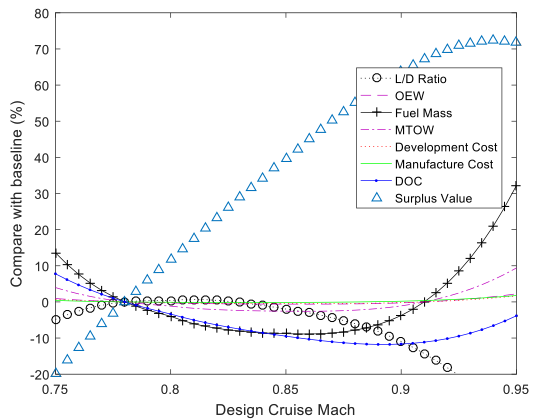
\includegraphics[width=0.8\textwidth]{./media4/mach.png}
  \caption{机翼梢根比的敏感性分析}
  \label{fig:mach}
\end{figure}

从图\ref{fig:mach}中可以得知,飞机的设计马赫数对不同属性有着不同的影响,飞机的空机重量对设计马赫数的敏感性较低,因此飞机的研发成本与制造成本变化不明显。当飞机的巡航马赫数增加,飞机的升阻比先下降后上升,因为当飞机的马赫数增加到一定数值会引发激波阻力,进而使得飞机的升阻比下降。由于飞机的气动特性的改变,使得飞机的燃油消耗先下降后快速上升,飞机的最大起飞重量受到燃油重量的影响,同样先下降后上升。飞机的直接使用成本受到燃油消耗以及重量的影响,随着马赫数的增加,飞机的直接使用成本先下降后上升,而飞机的剩余价值先增加后减少。

\item \textbf{机翼后掠角对飞机设计的影响}

后掠角是机翼的关键参数,机翼后掠角的大小对飞机的气动,结构与经济性都有很大的影响。飞机后掠角对飞机设计的影响如图\ref{fig:sweep}所示。

\begin{figure}[htp]
  \centering
  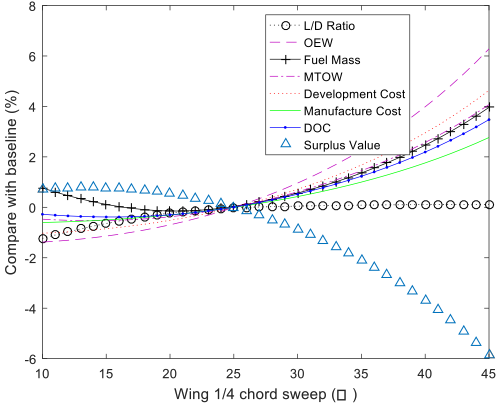
\includegraphics[width=0.75\textwidth]{./media4/sweep.png}
  \caption{飞机后掠角的相关敏感性分析}
  \label{fig:sweep}
\end{figure}

从图\ref{fig:sweep}可以看到,随着机翼后掠角的增加,飞机的空机重量增加,进而导致飞机的研发成本与制造成本增加。机翼后掠角的增加使得飞机的升阻比先增加后趋于平稳。当飞机的后掠角较小时,飞机的重量随着后掠角的增加而增加,飞机重量增加带来的影响小于气动特性的改善,因此飞机的燃油消耗改善。当飞机的后掠角较大时,飞机的气动特性趋于平稳,然而飞机的重量在增加,因此飞机的燃油消耗增加。燃油消耗总体呈先下降后上升趋势,直接使用成本随后掠角增加而上升,飞机的剩余价值先上升后下降。
\end{enumerate}


\subsection{环境参数对飞机设计的影响}
商用飞机从设计伊始到退出市场运营,这一过程受到众多环境因素的影响,商用飞机的经济性评估也受到环境因素的影响。在商用飞机的概念设计阶段就对这些环境参数进行考虑能够得到更加全面以及具有前瞻性的飞机设计方案。本节将对飞机的部分环境参数对飞机设计与评估的影响进行探索,搭建了与环境参数耦合的飞机设计程序,并将对环境参数进行相关飞机属性的敏感性分析。


飞机设计中相关的环境影响因素包括航空公司的运营参数的影响,机场环境参数的影响,航线网络参数的影响,宏观经济环境参数的影响,制造商运营参数的影响以及与设计活动相关参数的影响。本章将研究将环境参数与飞机设计相耦合的方法以及对相关的环境参数进行敏感性分析。

%%%%%%%%%%%%%%%%%%%% Figure/Image No: 1 starts here %%%%%%%%%%%%%%%%%%%%

\begin{figure}[ht!]
	\centering
	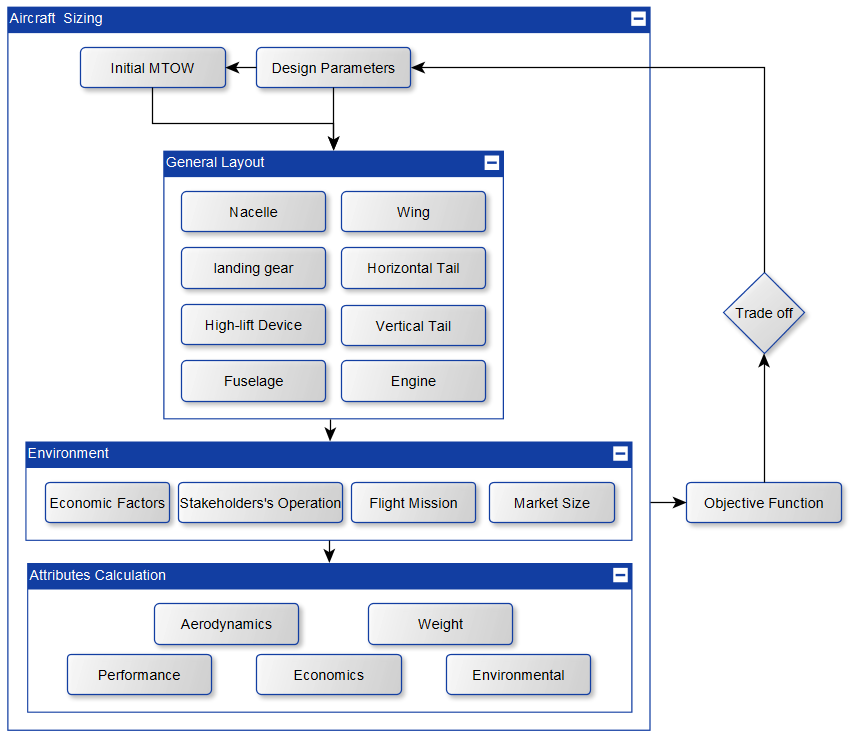
\includegraphics[width=4.06in,height=3.5in]{./media511/image1.png}
	\caption{与环境参数耦合的飞机设计程序}
	\label{fig:scenario}
\end{figure}

本研究搭建了与飞机设计环境相互耦合的飞机设计框架,如图\ref{fig:scenario}所示。在图中,在对飞机属性的评估之前,包括飞机气动,性能,重量,环保性以及飞机的经济性的估算,首先需要定义并且量化一组环境参数,用这一组环境参数搭建一个完整的环境,进而计算飞机的这些属性。

\subsubsection{航空公司运营参数的影响}
航空公司的运营参数,包括飞机的年飞行小时数,座位数与座位布局,机票价格,乘务人员的数量配置等。这些参数会对飞机的经济性评估产生影响,进而对飞机设计方案的权衡与优化产生影响。

\begin{enumerate}

\item \textbf{飞机的年飞行小时数}

飞机的年飞行小时数会影响飞机利用率与直接使用成本,进而对飞机的剩余价值产生影响,年飞行小时数对飞机经济性的影响如图\ref{fig:utilization}所示。

\begin{figure}[ht!]
	\centering
	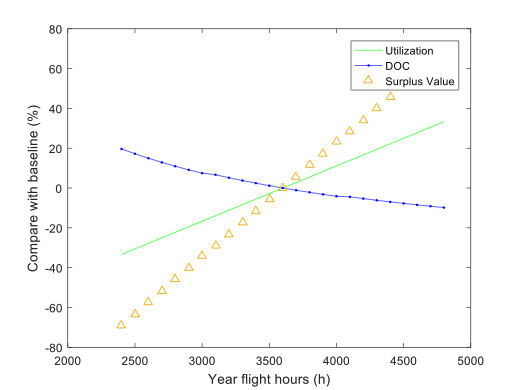
\includegraphics[width=0.8\textwidth]{./media511/utilization.png}
	\caption{年飞行小时数对飞机经济性的影响}
	\label{fig:utilization}
\end{figure}

在图\ref{fig:utilization}中,飞机的年飞机小时数的变化对飞机的利用率产生直接的影响,飞机的利用率随着年飞行小时数的增加而增加。飞机每趟飞行的直接使用成本随着年飞行小时数的增加而递减。在剩余价值的计算中,飞机的利用率对剩余价值的计算产生直接的影响,因此剩余价值随着飞机年飞行小时数的增加而增加。

\item \textbf{设计座位数}
\end{enumerate}

飞机的座位数会对飞机的制造成本与运营成本产生影响,同时也对飞机的盈利性产生影响。飞机的设计座位数对飞机设计的影响如图5-3所示。

\begin{figure}[ht!]
	\centering
	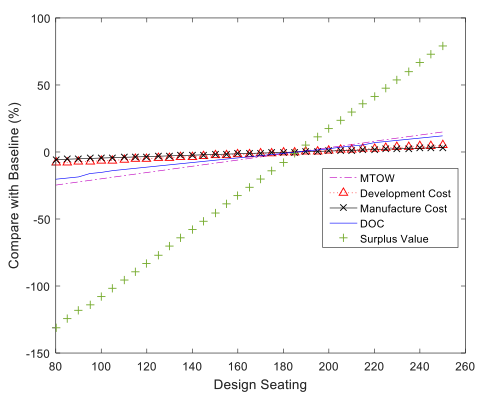
\includegraphics[width=0.75\textwidth]{./media511/seats.png}
	\caption{设计座位数的影响}
	\label{fig:seats}
\end{figure}

从图\ref{fig:seats}可以得出,飞机的座位数对飞机的重量产生影响,进而对飞机的研发成本与制造成本产生影响。设计座位数增加,飞机的空机重量与最大起飞重量增加,飞机的研发成本与制造成本上升。飞机的座位数增加,飞机的运行成本上升。当飞机的座位数增加,保持机票价格不变,飞机的剩余价值并没有因为重量,研发成本,制造成本以及使用成本的增加而减少。相反,飞机座位数的增加使得飞机盈利性增加对剩余价值的增益大于重量与成本增加所带来的负面影响,因此飞机的剩余价值提升。

\subsubsection{宏观经济性环境的影响}
\addcontentsline{toc}{subsubsection}{宏观经济性环境的影响}
宏观经济环境的相关参数会对飞机设计产生影响,这些影响参数包括汇率,物价上涨指数,航空燃油价格等参数,这些参数不会对飞机设计产生直接影响,但是会对飞机的经济性评估产生影响,进而影响对飞机设计方案的权衡与优化。

\begin{enumerate}
\item \textbf{汇率对飞机经济性的影响}

当我们用该DOC计算方法计算国内直接使用成本的经济性的时候,需用进行单位转换。汇率对飞机经济性的影响如图\ref{fig:exchange}所示。

\begin{figure}[ht!]
	\centering
	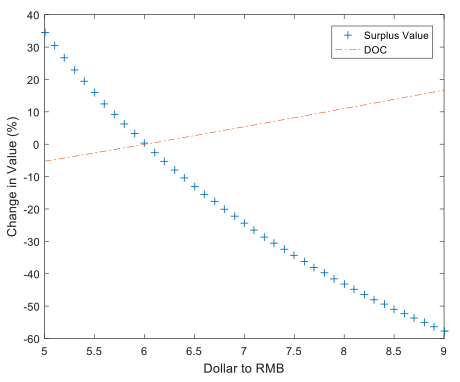
\includegraphics[width=0.7\textwidth]{./media512/exchangerate.png}
	\caption{汇率变化对飞机经济性的影响}
	\label{fig:exchange}
\end{figure}

图\ref{fig:exchange}中,飞机的直接使用成本随着汇率的提升而增加,而剩余价值随着汇率的增加而下降。采用AEA的方法进行国内DOC的估算需要进行汇率的转化。这中间涉及的成本项目计算包括机组人员的工资,维修材料成本的计算,维修劳务成本的计算等。

\item \textbf{航空燃油价格对飞机经济性的影响}

航空燃油价格处于时刻变动中,而飞机的燃油成本占据使用成本很大的比重,因此飞机的使用经济性对航空燃油价格十分敏感,航空燃油价格对飞机经济性的影响如图\ref{fig:rangefueprice}所示。

\begin{figure}[ht!]
	\centering
	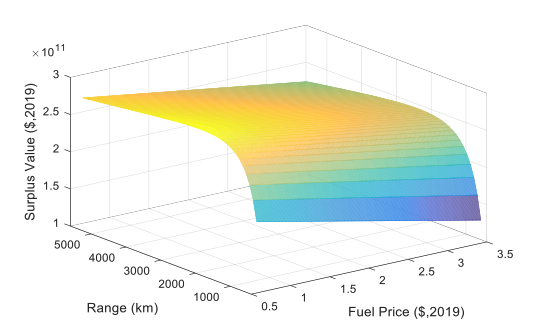
\includegraphics[width=0.7\textwidth]{./media512/range-fuelprice.png}
	\caption{航程与燃油价格对剩余价值的影响}
	\label{fig:rangefueprice}
\end{figure}
图\ref{fig:rangefueprice}中,飞机的剩余价值随着燃油成本的增加而下降,因为燃油成本的提升增加了飞机的使用成本,进而导致飞机的剩余价值下降。可以看到燃油价格的变化对飞机剩余价值产生显著的影响。结合近20年航空燃油价格数据的剧烈波动,如图\ref{fig:range-fuel}所示。因此在飞机的设计过程中对飞机设计方案的经济性评估需要对航空燃油价格进行合理考虑。

\begin{figure}[H]
	\centering
	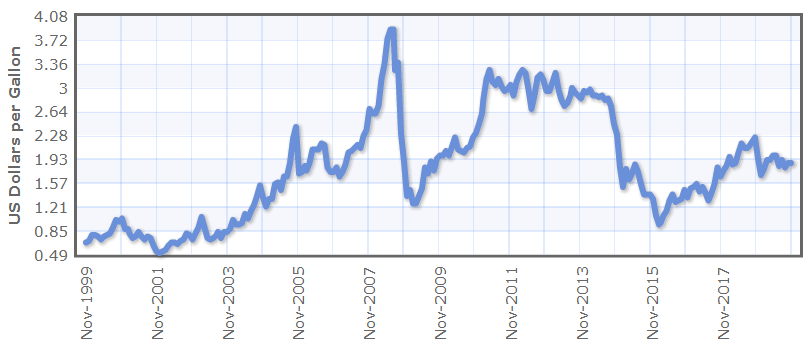
\includegraphics[width=0.8\textwidth]{./media512/image3.png}
	\caption{近20年的燃油价格的变化}
	\label{fig:range-fuel}
\end{figure}

\item \textbf{物价上涨指数对飞机经济性的影响}
物价上涨指数会影响飞机的研发成本与制造成本,物价上涨指数对飞机经济性的影响如图\ref{fig:cpi}所示。
\begin{figure}[hb]
	\centering
	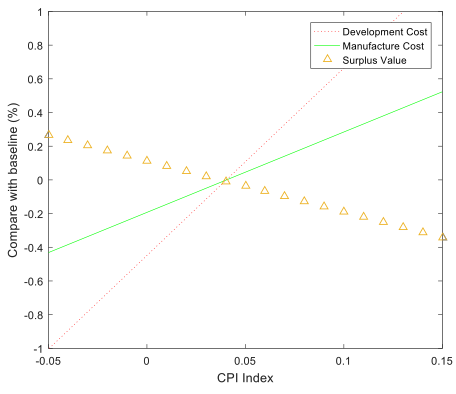
\includegraphics[width=0.7\textwidth]{./media512/cpi.png}
	\caption{物价上涨指数对飞机经济性的影响}
	\label{fig:cpi}
\end{figure}
从图\ref{fig:cpi}可以看到,飞机的研发成本与制造成本随着物价上涨指数的增加而增加,因此飞机的剩余价值下降,物价上涨指数的增加并不利于飞机的经济性。
\end{enumerate}

\subsubsection{制造商生产参数的影响}
\addcontentsline{toc}{subsubsection}{制造商生产参数的影响}
飞机制造商的相关运营参数,包括飞机生产数量,飞机生产率,折扣率与折扣系数等参数,这些参数不会对飞机的参数产生直接影响,但是会影响相关的飞机设计属性,包括飞机的经济性,进而影响对飞机设计方案的权衡。

\begin{enumerate}
\item \textbf{生产数量的影响}

飞机的单击成本随着产量的增加而下降,飞机制造商只有在到达一定的产量之后才会到达盈亏平衡点进而盈利。飞机的产量对经济性的影响如图\ref{fig:production}所示。

\begin{figure}[ht!]
	\centering
	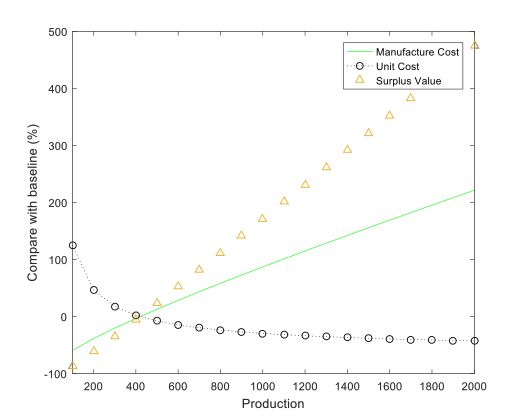
\includegraphics[width=0.8\textwidth]{./media512/production.png}
	\caption{飞机年产量对飞机经济性的影响}
	\label{fig:production}
\end{figure}

从图\ref{fig:production}可以得出,飞机的制造成本随着产量的增加而增加,而飞机的单机成本随产量的增加而减少,因为产量的提升均摊了固定成本。由于产量的提升以及单机成本的下降,飞机的剩余价值得以提升。

\item \textbf{飞机制造商折扣率与投资期限的影响}
\end{enumerate}

在剩余价值的计算中需要考虑飞机制造商的折扣系数以及航空公司的折扣系数,折扣系数直接影响了飞机的剩余价值,而折扣率与投资期限则通过影响飞机的折扣率进而改变飞机的剩余价值。其中制造商与投资期限对剩余价值的影响如图\ref{fig:discount}所示。

\begin{figure}[H]
	\centering
	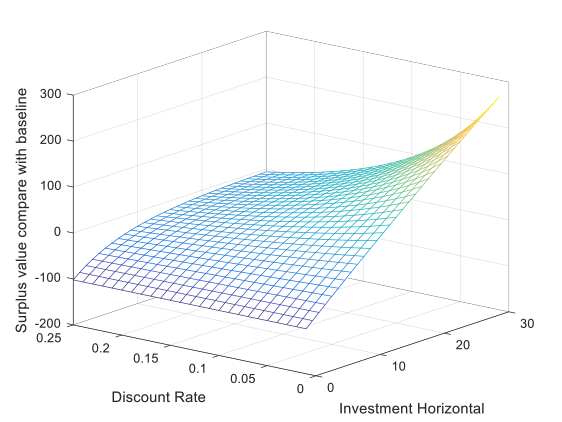
\includegraphics[width=0.8\textwidth]{./media512/discount.png}
	\caption{飞机制造商的折扣率与投资期限对剩余价值的影响}
	\label{fig:discount}
\end{figure}
图\ref{fig:discount}中,飞机的剩余价值同时受到折扣率与投资期限的影响,当飞机的折扣率较小时,飞机的剩余价值随着投资期限的增加而增加;当折扣率较大的时候,剩余价值随着投资期限的增加缓慢增加。

\subsection{发动机参数的影响}

如前一节所述,商用飞机研制中针对发动机选型问题,通常面临单选发动机还是多选发动机的问题,例如A320飞机可以安装的发动机包括CFM56,V2500,PW6000等。在本项目中,通过将发动机主要参数和飞机方案设计的程序相关联,用于发动机参数对价值函数的影响研究,这一结果可以满足在方案评估中的需求。

\begin{enumerate}
\item \textbf{发动机涵道比对飞机设计的影响}

发动机相关参数的改变将对飞机的重量与气动特性产生影响,进而影响飞机方案的经济性,需要和飞机的参数一并开展优化。发动机的性能影响飞机的燃油消耗,飞机的燃油消耗是飞机经济性的关键指标之一。本节分别考虑了发动机涵道比和油耗(SFC)对飞机相关价值函数和经济性指标的影响。通过飞机设计程序可以定量研究发动机涵道比和燃油效率对飞机设计的影响。

\begin{figure}[htp]
  \centering
  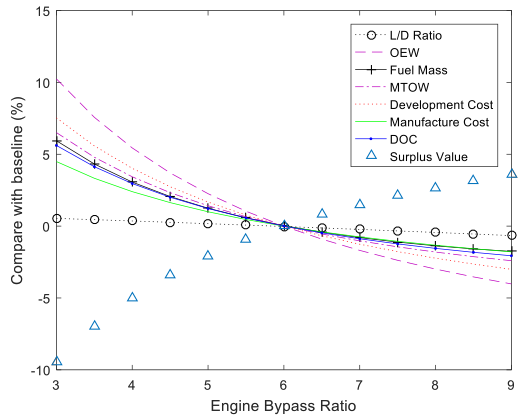
\includegraphics[width=0.8\textwidth]{./media4/bypassratio.png}
  \caption{发动机涵道比参数的影响}
  \label{fig:bypassratio}
\end{figure}
从图\ref{fig:bypassratio}中可以看到,飞机的重量随着涵道比的增加而下降,进而使得飞机的研发成本与制造成本下降。除此之外,由于飞机重量的下降以及飞机燃油消耗的改善,飞机的直接使用成本下降,飞机的剩余价值随着涵道比的增加而增加。
\end{enumerate}

图\ref{fig:sfc}给出了发动机油耗水平对飞机价值函数的影响,考虑到发动机燃油效率的历史规律和未来发展趋势,可以得到对飞机价值函数预期变化的估算。
\begin{figure}[htp]
  \centering
  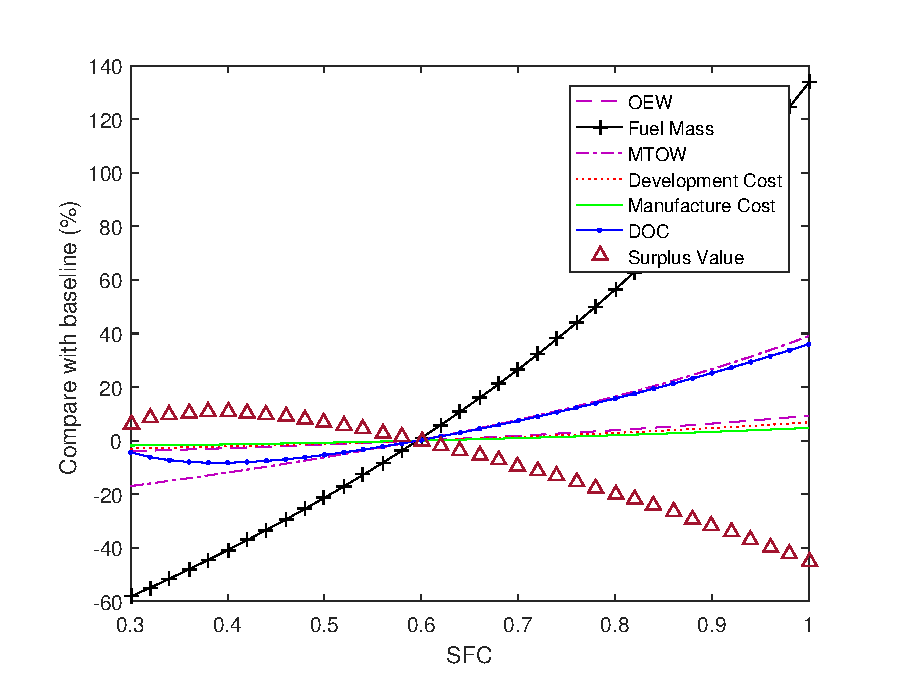
\includegraphics[width=0.8\textwidth]{./media4/SFC.eps}
  \caption{发动机油耗的影响}
  \label{fig:sfc}
\end{figure}

\subsection{本章小结}
\addcontentsline{toc}{subsection}{本章小结}

本节利用价值驱动设计理念进行飞机的设计方案的评估与优化,分别建立了以剩余价值和直接使用成本两个目标函数进行飞机方案设计的优化,包括飞机参数和发动机参数,并对比了两种单目标经济性优化方案的异同。此外兼顾了剩余价值与直接使用成本,对飞机进行多目标优化设计,提升了飞机的使用经济性与产业经济性,得到平衡与综合最优的飞机设计方案。除此之外,通过飞机设计程序研究相关飞机设计参数对飞机设计的影响,更加清楚地展示了飞机设计多学科之间的耦合关系。

本节研究了飞机环境参数与飞机方案设计流程的耦合,分别探索了航空公司运营参数,宏观经济环境参数,制造商生产参数与设计活动部分参数对飞机经济性的敏感性分析,结果表明不同的环境参数对飞机的方案评估产生不同的影响。除此之外,本章以航空公司的设计运营与座位数为例,探索了相关运营参数对飞机方案优化设计的影响,结果表明,不同的运营场景将产生截然不同的飞机方案优化设计。本章对部分环境参数的飞机经济敏感性分析以及部分环境参数对飞机设计的影响表明在飞机的设计过程中对飞机运行场景以及其他环境条件的合理考虑至关重要。


\chapter{主要宽体飞机及发动机数据}


\begin{landscape}
\tiny
\begin{center}
%\begin{figure}[htp]
%  \centering
%  \includegraphics[width=1.3\textwidth ]{bill.eps}\\
%  \caption{起落架典型部件及成本数据\cite{milwitzky1953analysis}}
%  \label{fig_bill}
%\end{figure}
% bill of materials and costing
\begin{longtable}{|p{1.5cm}|p{1.3cm}|p{1.1cm}|p{1.1cm}|p{1.1cm}|p{1.1cm}|p{1.1cm}|p{1.1cm}|p{1.1cm}|p{1.1cm}|p{1.1cm}|p{1.1cm}|p{1.1cm}|}
\caption{2000-2020典型宽体飞机数据} \\
\label{fig_widebody} \\
\hline 
%\begin{tabular}{|p{2cm}|p{1cm}|p{1.5cm}|p{2.5cm}|p{1cm}|p{1.5cm}|p{1.2cm}|p{1.5cm}|p{1.5cm}|p{1.2cm}|p{1.2cm}|}
%\begin{tabular}{|p{0.5cm}|p{2.0cm}|p{0.5cm}|p{1.5cm}|p{2.5cm}|l|l|l|p{1.5cm}|p{1.5cm}|p{1.2cm}|p{1.2cm}|}
机型	& B777-100X1 & 777-100X2 & 777-200X1 & 777-200X2	& A340-500	& A340-600	& A380-800	& 787-8	& A350-900	& 787-9	& A350-1000& 	787-10 \\ \hline
%零件 & 数量 & 零件编号 & 工艺 & 材料 & 材料名称 & 容积/$m^3$ & 材料成本($\pounds$)  & 制造成本($\pounds/kg$) & 人工成本(时薪)& 成本($\pounds$)\\ \hline
\endfirsthead
\multicolumn{4}{l}
{\tablename\ \thetable\ -- \textit{续前页}} \\
\hline
机型	& B777-100X1 & 777-100X2 & 777-200X1 & 777-200X2	& A340-500	& A340-600	& A380-800	& B787-8	& A350-900	& B787-9	& A350-1000& B787-10  \\ \hline
\endhead
制造商	&	BOEING	&	BOEING	&	BOEING	&	BOEING	&	AIRBUS	&	AIRBUS	&	AIRBUS	&	BOEING	&	AIRBUS	&	BOEING	&	AIRBUS	&	BOEING	\\ \hline
最早服役时间	&	2000	&	2000	&	2000	&	2000	&	2002	&	2002	&	2007	&	2011	&	2013	&	2014	&	2015	&	2018	\\ \hline
当前在役数量(预订数量)	&		&		&		&		&		&		&		&		&		&		&		&		\\ \hline
非洲	&	-	&	-	&	-	&	-	&	--->	&	(2)	&		&		&		&		&		&		\\ \hline
中东/亚洲/环太平洋	&	-	&	-	&	-	&	-	&	--->	&	(6)	&		&		&		&		&		&		\\ \hline
欧洲、独联体	&	-	&	-	&	-	&	-	&	--->	&	(27)	&		&		&		&		&		&		\\ \hline
美洲	&	-	&	-	&	-	&	-	&	--->	&	(5)	&		&		&		&		&		&		\\ \hline
总计	&	-	&	-	&	-	&	-	&	--->	&	(40)	&		&		&		&		&		&		\\ \hline
发动机制造商	&	R-R/GE/PW	&	R-R/GE/PW	&	R-R/GE/PW	&	R-R/GE/PW	&	R-R	&	R-R	&	R-R/Alliance	&	R-R/GE	&	R-R	&	R-R/GE	&	R-R	&	R-R/GE	\\ \hline
系列/型号	&	Options	&	Options	&	Options	&	Options	&	Trent 553	&	Trent 556	&	Trent970/GP7270	&	Trent1000/GEnx	&	Trent XWB	&	Trent1000/GEnx	&	Trent XWB	&	Trent1000/GEnx	\\ \hline
发动机数量	&	2	&	2	&	2	&	2	&	4	&	4	&	2	&	2	&	2	&	2	&	2	&	2	\\ \hline
静推力(kN)	&	400.0	&	400.0	&	413.8	&	436.0	&	235.8	&	249.1	&	356.8	&	280.0	&	387.0	&	320.0	&	422.0	&	340.0	\\ \hline
运营条款	&		&		&		&		&		&		&		&		&		&		&		&		\\ \hline
机舱	&		&		&		&		&		&		&		&		&		&		&		&		\\ \hline
最大座位数(单舱)	&	330	&	330	&	440	&	440	&	440	&	475	&	853	&	359	&	420	&	406	&	475	&	440	\\ \hline
两舱布局	&	271	&	250	&	375	&	375	&	350	&	440	&	575	&	248	&	314	&	290	&	350	&	330	\\ \hline
三舱布局	&	271	&	250	&	298	&	298	&	313	&	380	&	525	&	242	&	314	&	280	&	350	&	330	\\ \hline
并排座位数	&	9	&	9	&	10	&	10	&	9	&	9	&		&	9	&	10	&	9	&	10	&	9	\\ \hline
货舱空间	&		&		&	160.00	&	160.00	&	134.10	&	187.74	&		&	68.07	&	113.00	&	75.38	&	113.00	&	81.90	\\ \hline
人均空间	&		&		&	0.36	&	0.36	&	0.30	&	0.40	&		&	0.19	&		&	0.19	&		&	0.19	\\ \hline
质量(重量)(kg)	&		&		&		&		&		&		&		&		&		&		&		&		\\ \hline
停机坪重量	&		&		&		&		&	365900	&	365900	&	562000	&		&	268900	&		&	308900	&		\\ \hline
最大起飞重量	&	286621	&	299320	&	299320	&	312925	&	365000	&	365000	&	575155	&	227900	&	265000	&	254000	&	295000	&	254000	\\ \hline
最大着陆重量	&		&		&		&		&	236000	&	254000	&	386000	&	172400	&	202000	&	192800	&	225500	&	201800	\\ \hline
零油重量	&		&		&		&		&	222000	&	240000	&	361000	&	16100	&	192000	&	181400	&	220000	&	192800	\\ \hline
最大有效载荷	&		&		&		&		&	51635	&	63000	&	83915	&	62959	&	53300	&	63958	&	68000	&		\\ \hline
最大燃油裁量	&		&		&		&		&	31450	&	29311	&		&		&		&		&		&		\\ \hline
设计有效载荷	&	25745	&	23750	&		&		&	29735	&	36100	&		&	41440	&		&	42722	&		&		\\ \hline
设计燃油载量	&		&		&		&		&	164875	&	151890	&		&		&		&		&		&		\\ \hline
使用空重	&		&		&		&		&	170390	&	177010	&	277145	&	119950	&	142400	&	128800	&	155000	&	135500	\\ \hline
重量比	&		&		&		&		&		&		&		&		&		&		&		&		\\ \hline
飞机使用空重/最大起飞重量	&		&		&		&		&	0.467	&	0.485	&	0.482	&		&	0.537	&		&	0.525	&		\\ \hline
最大有效载荷/最大起飞重量	&		&		&		&		&	0.141	&	0.173	&		&		&		&		&		&		\\ \hline
最大燃油重量/最大起飞重量	&		&		&		&		&	0.423	&	0.423	&		&		&		&		&		&		\\ \hline
最大着陆重量/最大起飞重量	&		&		&		&		&	0.647	&	0.696	&	0.671	&		&	0.762	&		&	0.764	&		\\ \hline
燃油(升)	&		&		&		&		&		&		&		&		&		&		&		&		\\ \hline
标配燃油	&		&		&	174735	&	174735	&	195620	&	195620	&	310000	&	126200	&	150000	&	126370	&	150000	&	126370	\\ \hline
可附加燃油	&		&		&		&		&	213120	&		&	320000	&		&		&		&		&		\\ \hline
尺寸	&		&		&		&		&		&		&		&		&		&		&		&		\\ \hline
机身	&		&		&		&		&		&		&		&		&		&		&		&		\\ \hline
长度(m)	&	56.40	&	59.60	&	62.78	&	62.78	&	65.60	&	69.57	&	72.72	&	56.70	&	66.80	&	62.80	&	73.79	&	68.30	\\ \hline
高度(m)	&	6.20	&	6.20	&	6.20	&	6.20	&	5.64	&	5.64	&	8.41	&	5.94	&	6.09	&	5.94	&	6.09	&	5.94	\\ \hline
宽度(m)	&	6.20	&	6.20	&	6.20	&	6.20	&	5.64	&	5.64	&	7.14	&	5.77	&	5.96	&	5.77	&	5.96	&	5.77	\\ \hline
长细比	&	9.10	&	9.61	&	10.13	&	10.13	&	11.63	&	12.34	&	10.18	&	9.83	&	11.21	&	10.88	&	12.38	&	11.84	\\ \hline
机翼	&		&		&		&		&		&		&		&		&		&		&		&		\\ \hline
参考面积($m^2$)	&	427.80	&	427.80	&	427.80	&	427.80	&	437.30	&	437.30	&	845.00	&	360.50	&	443.00	&	360.50	&	443.00	&	360.50	\\ \hline
翼展(m)	&	60.90	&	60.90	&	60.90	&	60.90	&	61.20	&	61.20	&	79.75	&	60.00	&	64.00	&	60.10	&	64.00	&	60.10	\\ \hline
平均空气动弦长(m)	&	8.75	&	8.75	&	8.75	&	8.75	&	8.35	&	8.35	&		&	6.27	&		&	6.27	&		&	6.27	\\ \hline
展弦比	&	8.67	&	8.67	&	8.67	&	8.67	&	8.56	&	8.56	&	7.53	&	9.59	&	9.49	&	9.59	&	9.03	&	9.59	\\ \hline
梢根比	&	0.149	&	0.149	&	0.149	&	0.149	&	0.220	&	0.220	&	0.260	&		&		&		&		&		\\ \hline
1/4弦长后掠角 (º)	&	31.60	&	31.60	&	31.60	&	31.60	&	31.10	&	31.10	&	33.50	&	32.20	&	35.00	&	36.00	&	35.00	&	40.00	\\ \hline
平均$t/c$ %	&		&		&		&		&		&		&	8.00	&		&		&		&		&		\\ \hline
增升装置	&		&		&		&		&		&		&		&		&		&		&		&		\\ \hline
后缘襟翼类型	&	S2/S1	&	S2/S1	&	S2/S1	&	S2/S1	&	S2	&	S2	&		&		&		&		&		&		\\ \hline
襟翼展向百分比	&	0.758	&	0.758	&	1.758	&	2.758	&	0.625	&	0.625	&		&		&		&		&		&		\\ \hline
襟翼面积($m^2$)	&		&		&		&		&		&		&		&		&		&		&		&		\\ \hline
前缘襟翼类型	&	slats	&	slats	&	slats	&	slats	&	slats	&	slats	&		&		&		&		&		&		\\ \hline
翼面积($m^2$)	&		&		&		&		&		&		&		&		&		&		&		&		\\ \hline
垂直尾翼	&		&		&		&		&		&		&		&		&		&		&		&		\\ \hline
尾翼面积($m^2$)	&	53.23	&	53.23	&	53.23	&	53.23	&	47.65	&	47.65	&		&		&		&		&		&		\\ \hline
高度($m$)	&	9.24	&	9.24	&	9.24	&	9.24	&	9.44	&	9.44	&		&		&		&		&		&		\\ \hline
展弦比	&	1.60	&	1.60	&	1.60	&	1.60	&	1.87	&	1.87	&		&		&		&		&		&		\\ \hline
梢根比	&	0.290	&	0.290	&	0.290	&	0.290	&	0.350	&	0.350	&		&		&		&		&		&		\\ \hline
$1/4$弦长后掠角 ($^\circ$)	&	46.00	&	46.00	&	46.00	&	46.00	&	45.00	&	45.00	&		&		&		&		&		&		\\ \hline
垂尾力臂($m$)	&	23.41	&	25.01	&	26.60	&	26.60	&	27.50	&	27.50	&		&		&		&		&		&		\\ \hline
Sv/S	&	0.124	&	0.124	&	0.124	&	0.124	&	0.109	&	0.109	&		&		&		&		&		&		\\ \hline
SvLv/Sb	&	0.048	&	0.051	&	0.054	&	0.054	&	0.049	&	0.049	&		&		&		&		&		&		\\ \hline
水平尾翼	&		&		&		&		&		&		&		&		&		&		&		&		\\ \hline
翼面积($m^2$)	&	101.26	&	101.26	&	101.26	&	101.26	&	93.00	&	93.00	&		&		&		&		&		&		\\ \hline
翼展(m)	&	21.35	&	21.35	&	21.35	&	21.35	&	21.50	&	21.50	&		&		&		&		&		&		\\ \hline
展弦比	&	4.50	&	4.50	&	4.50	&	4.50	&	4.97	&	4.97	&		&		&		&		&		&		\\ \hline
梢根比	&	0.300	&	0.300	&	0.300	&	0.300	&	0.360	&	0.360	&		&		&		&		&		&		\\ \hline
1/4弦长处后掠角 ($^\circ$)	&	35.00	&	35.00	&	35.00	&	35.00	&	30.00	&	30.00	&		&		&		&		&		&		\\ \hline
平尾力臂($m$)	&	24.71	&	26.31	&	27.90	&	27.90	&	28.60	&	28.60	&		&		&		&		&		&		\\ \hline
Sh/S	&	0.237	&	0.237	&	0.237	&	0.237	&	0.213	&	0.213	&		&		&		&		&		&		\\ \hline
ShLh/Sc	&	0.668	&	0.712	&	0.755	&	0.755	&	0.729	&	0.729	&		&		&		&		&		&		\\ \hline
起落架	&		&		&		&		&		&		&		&		&		&		&		&		\\ \hline
起落架轮距($m$)	&	11.00	&	11.00	&	11.00	&	11.00	&	10.70	&	10.70	&	14.30	&		&	10.60	&		&	10.70	&		\\ \hline
前后车轮轴距($m$)	&	25.80	&	25.80	&	25.80	&	25.80	&	28.53	&	32.50	&	30.40	&		&	28.67	&		&	33.10	&		\\ \hline
转弯半径($m$)	&	41.00	&	41.00	&	41.00	&	41.00	&		&		&		&		&		&		&		&		\\ \hline
车轮数量(前;后)	&	2;12	&	2;12	&	2;12	&	2;12	&	2;12	&	2;12	&		&		&		&		&		&		\\ \hline
主轮直径($m$)	&	1.118	&	1.118	&	1.118	&	1.118	&		&		&		&		&		&		&		&		\\ \hline
主轮宽度($m$)	&	0.457	&	0.457	&	0.457	&	0.457	&		&		&		&		&		&		&		&		\\ \hline
引擎机舱	&		&		&		&		&		&		&		&		&		&		&		&		\\ \hline
长度($m$)	&	7.30	&	7.30	&	7.30	&	7.30	&	6.10	&	6.10	&		&		&		&		&		&		\\ \hline
最大宽度($m$)	&	3.20	&	3.20	&	3.20	&	3.20	&	3.05	&	3.05	&		&		&		&		&		&		\\ \hline
展向位置	&	0.326	&	0.326	&	0.326	&	0.326	&	0.296/0.625	&	0.296/0.625	&		&		&		&		&		&		\\ \hline
性能	&		&		&		&		&		&		&		&		&		&		&		&		\\ \hline
载重	&		&		&		&		&		&		&		&		&		&		&		&		\\ \hline
最大功率负荷($kg/kN$)	&	358.28	&	374.15	&	361.67	&	358.86	&	386.98	&	366.32	&		&		&		&		&		&		\\ \hline
最大翼载($kg/m^2$)	&	669.99	&	699.67	&	699.67	&	731.47	&	834.67	&	834.67	&		&		&		&		&		&		\\ \hline
推重比	&	0.2845	&	0.2724	&	0.2818	&	0.2841	&	0.2634	&	0.2783	&		&		&		&		&		&		\\ \hline
起飞距离($m$)	&		&		&		&		&		&		&		&		&		&		&		&		\\ \hline
ISA 海平面	&		&		&		&		&	3100	&	3100	&	2050	&	2600	&	2600	&	2800	&	2600	&	2800	\\ \hline
ISA +20$^\circ C$ 海平面	&		&		&		&		&	3550	&	3550	&		&		&		&		&		&		\\ \hline
ISA 5000ft	&		&		&		&		&	4250	&	4250	&		&		&		&		&		&		\\ \hline
ISA +20$^\circ C$C 5000ft	&		&		&		&		&		&		&		&		&		&		&		&		\\ \hline
着陆距离(m)	&		&		&		&		&		&		&		&		&		&		&		&		\\ \hline
ISA 海平面	&		&		&		&		&	2090	&	2240	&	2900	&	1737	&	2000	&		&	2000	&		\\ \hline
ISA +20$^\circ C$ 海平面	&		&		&		&		&	2090	&	2240	&		&		&		&		&		&		\\ \hline
ISA 5000ft	&		&		&		&		&	2390	&		&		&		&		&		&		&		\\ \hline
ISA +20$^\circ C$ 5000ft	&		&		&		&		&	2390	&		&		&		&		&		&		&		\\ \hline
速度(kt/Mach):	&		&		&		&		&		&		&		&		&		&		&		&		\\ \hline
V2	&		&		&		&		&		&		&		&		&		&		&		&		\\ \hline
Vapp	&		&		&		&		&	139	&	144	&		&		&		&		&		&		\\ \hline
Vno/Mmo	&		&		&		&		&	330/M0.86	&	330/M0.86	&	511/M0.95	&	350/M0.90	&		&	350/M0.90	&		&	350/M0.90	\\ \hline
Vne/Mme	&		&		&		&		&	365/M0.93	&	365/M0.93	&		&		&		&		&		&		\\ \hline
CLmax (T/O)	&		&		&		&		&		&		&		&		&		&		&		&		\\ \hline
CLmax (L/D @ MLM)	&		&		&		&		&	2.86	&	2.87	&		&		&		&		&		&		\\ \hline
最大巡航	&		&		&		&		&		&		&		&		&		&		&		&		\\ \hline
518	&		&		&		&		&		&		&	488	&	488	&	510	&	488	&	510	&	488	\\ \hline
高度(ft)	&		&		&		&		&		&		&		&	42979	&		&	42979	&		&	42979	\\ \hline
耗油率(kg/h)	&		&		&		&		&		&		&		&		&		&		&		&		\\ \hline
远程巡航	&		&		&		&		&		&		&		&		&		&		&		&		\\ \hline
速度(kt)	&		&		&		&		&		&		&		&	510	&		&	510	&		&	510	\\ \hline
高度(ft)	&		&		&		&		&		&		&		&		&		&		&		&		\\ \hline
耗油率(kg/h)	&		&		&		&		&		&		&		&		&		&		&		&		\\ \hline
航程(海里)	&		&		&		&		&		&		&		&		&		&		&		&		\\ \hline
最大载荷航程	&		&		&		&		&	7050	&	5700	&	15000	&	7343	&	15000	&	7613	&	14800	&	6425	\\ \hline
设计航程	&	7625	&	8420	&	7455	&	7970	&	8500	&	7500	&	14800?	&	7343	&		&	7530	&		&	6345	\\ \hline
最大燃油航程(+载荷)	&		&		&		&		&	9000	&	7800	&		&		&		&		&		&		\\ \hline
转场航程 	&		&		&		&		&	9800	&	8800	&		&		&		&		&		&		\\ \hline
设计参数	&		&		&		&		&		&		&		&		&		&		&		&		\\ \hline
W/SCLmax	&		&		&		&		&	2865.71	&	2857.63	&		&		&		&		&		&		\\ \hline
W/SCLtoST	&		&		&		&		&	4144.91	&	3912.54	&		&		&		&		&		&		\\ \hline
燃油/旅客	&		&		&		&		&	0.0554	&	0.0460	&		&		&		&		&		&		\\ \hline
座位数 x 航程	&		&		&		&		&	2975000	&	3300000	&		&		&		&		&		&		\\ \hline
\hline
%\hhline{|=|=|=|=|=|=|=|=|=|=|=|}
%\end{tabular}
\label{nosegearpars} 
\end{longtable}
\end{center}
\end{landscape}


\begin{landscape}
\tiny
\begin{center}
%\begin{figure}[htp]
%  \centering
%  \includegraphics[width=1.3\textwidth ]{bill.eps}\\
%  \caption{起落架典型部件及成本数据\cite{milwitzky1953analysis}}
%  \label{fig_bill}
%\end{figure}
% bill of materials and costing
\begin{longtable}{|p{1.5cm}|p{1.3cm}|p{1.1cm}|p{1.1cm}|p{1.1cm}|p{1.1cm}|p{1.1cm}|p{1.1cm}|p{1.1cm}|p{1.1cm}|p{1.1cm}|}
\caption{1990-2000典型宽体飞机数据} \\
\label{fig_widebody} \\
\hline 
%\begin{tabular}{|p{2cm}|p{1cm}|p{1.5cm}|p{2.5cm}|p{1cm}|p{1.5cm}|p{1.2cm}|p{1.5cm}|p{1.5cm}|p{1.2cm}|p{1.2cm}|}
%\begin{tabular}{|p{0.5cm}|p{2.0cm}|p{0.5cm}|p{1.5cm}|p{2.5cm}|l|l|l|p{1.5cm}|p{1.5cm}|p{1.2cm}|p{1.2cm}|}
机型	&	MD-11	&	A340-200	&	A340-300	&	A330-300	&	Il-96-300	&	B777-200	&	B777-200IGW	&	Il-96M	&	B777-300	&	A330-200\\ \hline
\endfirsthead
\multicolumn{4}{l}
{\tablename\ \thetable\ -- \textit{续前页}} \\
\hline
机型	&	MD-11	&	A340-200	&	A340-300	&	A330-300	&	Il-96-300	&	B777-200	&	B777-200IGW	&	Il-96M	&	B777-300	&	A330-200\\ \hline
\endhead
制造商	&	McDON.	&	AIRBUS	&	AIRBUS	&	AIRBUS	&	ILYUSHIN	&	BOEING	&	BOEING	&	ILYUSHIN	&	BOEING	&	AIRBUS \\ \hline
系列	&	DOUG.	&	A340-	&	A340-	&	A330-	&		&	777-	&	777-	&		&	777-	&	A330-\\ \hline
机型	&	MD-11	&	200	&	300	&	300	&	Il-96-300	&	200	&	200IGW	&	Il-96M	&	300	&	200\\ \hline
型号	&		&	A340-200	&	A340-300	&	A330-300	&		&	B777-200	&	B777-200IGW	&		&	B777-300	&	A330-200\\ \hline
最早服役时间	&	1990	&	1993	&	1994	&	1994	&	1994	&	1995	&	1995	&	1996	&	1998	&	1998\\ \hline
当前在役数量(预订数量)	&		&		&		&		&		&		&		&		&		&	\\ \hline
非洲	&	-	&	--->	&	8(1)	&	-	&	-	&	--->	&	3(4)	&	-	&	-	&	--->\\ \hline
中东/亚洲/环太平洋	&	46(3)	&	--->	&	54(10)	&	59(47)	&	-	&	--->	&	90(74)	&	-	&	11(37)	&	--->\\ \hline
欧洲、独联体	&	55(10)	&	--->	&	69(15)	&	17(42)	&	9 (9)	&	--->	&	26(39)	&	(23)	&	-	&	--->\\ \hline
美洲	&	77(3)	&	--->	&	9(8)	&	4(42)	&	-	&	--->	&	38(78)	&	-	&	-	&	--->\\ \hline
总计	&	178(16)	&	--->	&	140(34)	&	80(131)	&	9(9)	&	--->	&	157(195)	&	(23)	&	11(37)	&	--->\\ \hline
发动机制造商	&	GE	&	CFMI	&	CFMI	&	GE	&	Soloviev	&	R-R/GE/PW	&	R-R/GE/PW	&	PW	&	R-R	&	GE\\ \hline
系列/型号	&	CF6-80C2 D1F	&	CFM-56-5C2	&	CFM-56-5C4	&	CF6-80E1A2	&	PS-90A	&	Options	&	Options	&	2337	&	Trent 895	&	CF6-80E1A4\\ \hline
发动机数量	&	3	&	4	&	4	&	2	&	4	&	2	&	2	&	4	&	2	&	2\\ \hline
静推力(kN)	&	274.0	&	139.0	&	151.0	&	300.0	&	156.9	&	342.5	&	373.7	&	164.6	&	423.0	&	310.0\\ \hline
运营条款	&		&		&		&		&		&		&		&		&		&	\\ \hline
机舱	&		&		&		&		&		&		&		&		&		&	\\ \hline
最大座位数(单舱)	&	405	&	440	&	440	&	440	&	300	&	440	&	440	&	375	&	550	&	380\\ \hline
两舱布局	&	323	&	303	&	335	&	335	&		&	375	&	375	&	335	&	479	&	293\\ \hline
三舱布局	&	293	&	262	&	295	&	295	&	235	&	310	&	310	&	312	&	394	&	253\\ \hline
并排座位数	&	10	&	9	&	9	&	9	&	9	&	10	&	10	&	9	&	10	&	9\\ \hline
货舱空间	&	194.00	&	136.00	&	162.90	&	162.90	&	115.90	&	160.00	&	160.00	&	143.04	&	200.50	&	136.00\\ \hline
人均空间	&	0.48	&	0.31	&	0.37	&	0.37	&	0.39	&	0.36	&	0.36	&	0.38	&	0.36	&	0.36\\ \hline
质量(重量)(kg)	&		&		&		&		&		&		&		&		&		&	\\ \hline
停机重量	&	285081	&	257900	&	271900	&	233900	&		&	243577	&	287804	&		&	299600	&	233900\\ \hline
最大起飞重量	&	283720	&	257000	&	271000	&	233000	&	216000	&	242670	&	286897	&	270000	&	299370	&	233000\\ \hline
最大着陆重量	&	207744	&	181000	&	190000	&	187000	&	175000	&	201850	&	208652	&	175158	&	237685	&	182000 \\ \hline
零油重量	&	195043	&	172000	&	178000	&	175000	&	157000	&	190510	&	195045	&	190423	&	224530	&	170000\\ \hline
最大有效载荷	&	55566	&	49400	&	48150	&	48400	&	40000	&	54635	&	56925	&	58000	&	68570	&	36400\\ \hline
最大燃油裁量	&	30343	&	21220	&	33160	&	18600	&	0	&		&		&	17290.4	&		&	0\\ \hline
设计有效载荷	&	30685	&	24890	&	28025	&	28025	&	22325	&	35625	&	29450	&	29640	&		&	24035\\ \hline
设计燃油载量	&	118954	&	111882	&	113125	&	70786	&	76675	&	71170	&	119327	&	107960	&		&	85765\\ \hline
使用空重	&	134081	&	120228	&	129850	&	124500	&	117000	&	135875	&	138120	&	132400	&	155960	&	119600\\ \hline
重量比	&		&		&		&		&		&		&		&		&		&	\\ \hline
飞机使用空重/最大起飞重量	&	0.473	&	0.468	&	0.479	&	0.545	&	0.542	&	0.560	&	0.481	&	0.490	&	0.521	&	0.523\\ \hline
最大有效载荷/最大起飞重量	&	0.196	&	0.192	&	0.178	&	0.223	&	0.185	&	0.225	&	0.198	&	0.215	&	0.229	&	0.158\\ \hline
最大燃油重量/最大起飞重量	&	0.424	&	0.430	&	0.412	&	0.358	&	0.550	&	0.382	&	0.466	&	0.440	&	0.452	&	0.478\\ \hline
最大着陆重量/最大起飞重量	&	0.732	&	0.704	&	0.701	&	0.825	&	0.810	&	0.832	&	0.727	&	0.649	&	0.794	&	0.770\\ \hline
燃油($Litre$)	&		&		&		&		&		&		&		&		&		&	\\ \hline
标配燃油	&	152108	&	140000	&	141500	&	97170	&	150387	&	117348	&	169208	&	150387	&	171170	&	139090\\ \hline
可附加燃油	&	161226	&		&	148700	&		&		&		&		&		&		&	\\ \hline
尺寸	&		&		&		&		&		&		&		&		&		&	\\ \hline
机身	&		&		&		&		&		&		&		&		&		&	\\ \hline
长度($m$)	&	58.65	&	58.21	&	62.47	&	62.47	&	51.15	&	62.78	&	62.78	&	60.50	&	72.88	&	57.77\\ \hline
高度($m$)	&	6.02	&	5.64	&	5.64	&	5.64	&	6.08	&	6.20	&	6.20	&	6.08	&	6.20	&	5.64\\ \hline
宽度($m$)	&	6.02	&	5.64	&	5.64	&	5.64	&	6.08	&	6.20	&	6.20	&	6.08	&	6.20	&	5.64\\ \hline
长细比	&	9.74	&	10.32	&	11.08	&	11.08	&	8.41	&	10.13	&	10.13	&	9.95	&	11.75	&	10.24\\ \hline
机翼参考面积($m^2$)	&	338.90	&	363.10	&	363.10	&	363.10	&	391.60	&	427.80	&	427.80	&	391.60	&	427.80	&	363.10\\ \hline
翼展($m$)	&	51.77	&	58.00	&	58.00	&	58.00	&	55.57	&	60.90	&	60.90	&	55.57	&	60.90	&	58.00\\ \hline
平均空气动弦长($m$)	&	7.68	&	7.26	&	7.26	&	7.26	&	8.04	&	8.75	&	8.75	&	8.04	&	8.75	&	7.26\\ \hline
展弦比	&	7.91	&	9.26	&	9.26	&	9.26	&	7.89	&	8.67	&	8.67	&	7.89	&	8.67	&	9.26\\ \hline
梢根比	&	0.239	&	0.251	&	0.251	&	0.251	&	0.279	&	0.149	&	0.149	&	0.279	&	0.149	&	0.251\\ \hline
1/4弦长后掠角 ($^\circ$)	&	9.35	&	29.70	&	29.70	&	29.70	&		&	31.60	&	31.60	&		&	31.60	&	29.70\\ \hline
平均t/c 	&	35.00	&		&		&		&	30.00	&		&		&	30.00	&		&\\ \hline	
增升装置	&		&		&		&		&		&		&		&		&		&	\\ \hline
后缘襟翼类型	&	S2	&	S2	&	S2	&	S2	&	S2	&	S2/S1	&	S2/S1	&	S2	&	S2/S1	&	S2\\ \hline
襟翼展向百分比	&	0.700	&	0.665	&	0.665	&	0.665	&	0.790	&	0.758	&	0.758	&	0.790	&	2.758	&	0.665\\ \hline
襟翼面积($m^2$)	&		&		&		&		&		&		&		&		&		&	\\ \hline
前缘襟翼类型	&	slats	&	slats	&	slats	&	slats	&	slats	&	slats	&	slats	&	slats	&	slats	&	slats\\ \hline
翼面积($m^2$)	&		&		&		&		&		&		&		&		&		&	\\ \hline
垂直尾翼	&		&		&		&		&		&		&		&		&		&	\\ \hline
尾翼面积($m^2$)	&	56.20	&	45.20	&	45.20	&	45.20	&	61.00	&	53.23	&	53.23	&	56.20	&	53.23	&	47.65\\ \hline
高度($m$)	&	11.16	&	8.45	&	8.45	&	8.45	&	9.40	&	9.24	&	9.24	&	8.00	&	9.24	&	9.44\\ \hline
展弦比	&	2.22	&	1.58	&	1.58	&	1.58	&	1.45	&	1.60	&	1.60	&	1.14	&	1.60	&	1.87\\ \hline
梢根比	&	0.369	&	0.350	&	0.350	&	0.350	&	0.280	&	0.290	&	0.290	&	0.400	&	0.290	&	0.350\\ \hline
1/4弦长后掠角 ($^\circ$)	&	40.00	&	45.00	&	45.00	&	45.00	&	45.00	&	46.00	&	46.00	&	45.00	&	46.00	&	45.00\\ \hline
垂尾力臂($m$)	&	20.92	&	25.50	&	27.50	&	27.50	&	23.55	&	26.60	&	26.60	&	25.90	&	31.65	&	25.20\\ \hline
Sv/S	&	0.166	&	0.124	&	0.124	&	0.124	&	0.156	&	0.124	&	0.124	&	0.144	&	0.124	&	0.131\\ \hline
SvLv/Sb	&	0.067	&	0.055	&	0.059	&	0.059	&	0.066	&	0.054	&	0.054	&	0.067	&	0.065	&	0.057\\ \hline
水平尾翼	&		&		&		&		&		&		&		&		&		&	\\ \hline
翼面积($m^2$)	&	85.50	&	72.90	&	72.90	&	72.90	&	96.50	&	101.26	&	101.26	&	96.50	&	101.26	&	31.00\\ \hline
翼展($m$)	&	18.03	&	19.06	&	19.06	&	19.06	&	20.57	&	21.35	&	21.35	&	20.57	&	21.35	&	12.45\\ \hline
展弦比	&	3.80	&	4.98	&	4.98	&	4.98	&	4.38	&	4.50	&	4.50	&	4.38	&	4.50	&	5.00\\ \hline
梢根比	&	0.383	&	0.360	&	0.360	&	0.360	&	0.290	&	0.300	&	0.300	&	0.290	&	0.300	&	0.256\\ \hline
1/4弦长处后掠角 ($^\circ$)	&	35.00	&	30.00	&	30.00	&	30.00	&	37.50	&	35.00	&	35.00	&	37.50	&	35.00	&	29.00\\ \hline
平尾力臂($m$)	&	20.92	&	26.50	&	28.60	&	28.60	&	24.25	&	27.90	&	27.90	&	26.50	&	32.95	&	16.20\\ \hline
Sh/S	&	0.252	&	0.201	&	0.201	&	0.201	&	0.246	&	0.237	&	0.237	&	0.246	&	0.237	&	0.253\\ \hline
ShLh/Sc	&	0.687	&	0.733	&	0.791	&	0.791	&	0.743	&	0.755	&	0.755	&	0.812	&	0.891	&	0.957\\ \hline
起落架	&		&		&		&		&		&		&		&		&		&	\\ \hline
起落架轮距($m$)	&	10.60	&	10.70	&	10.70	&	10.70	&	10.40	&	11.00	&	11.00	&	10.40	&	11.00	&	7.60\\ \hline
前后车轮轴距($m$)	&	24.60	&	23.20	&	25.40	&	25.40	&	20.07	&	25.80	&	25.80	&	27.35	&	25.80	&	16.90\\ \hline
转弯半径($m$)	&	41.00	&		&	40.60	&	41.40	&		&	41.00	&	41.00	&		&	41.00	&	29.00\\ \hline
车轮数量(前;后)	&	2;10	&	2;10	&	2;10	&	2;8	&	2;8	&	2;12	&	2;12	&	2;8	&	2;12	&	2;8\\ \hline
主轮直径($m$)	&		&		&		&		&	1.300	&	1.118	&	1.118	&	1.300	&	1.118	&	\\ \hline
主轮宽度($m$)	&		&		&		&		&	0.480	&	0.457	&	0.457	&	0.480	&	0.457	&	\\ \hline
引擎机舱	&		&		&		&		&		&		&		&		&		&	\\ \hline
长度($m$)	&	6.50	&	4.95	&	4.95	&	7.00	&	5.90	&	7.30	&	7.30	&	6.00	&	7.30	&	7.00\\ \hline
最大宽度($m$)	&	2.70	&	2.37	&	2.37	&	3.10	&	2.20	&	3.20	&	3.20	&	2.60	&	3.20	&	3.10\\ \hline
展向位置	&	0.308	&	0.312/0.672	&	0.312/0.672	&	0.312	&	0.37/0.58	&	0.326	&	0.326	&	0.37/0.58	&	0.326	&	0.312\\ \hline
性能	&		&		&		&		&		&		&		&		&		&	\\ \hline
载重	&		&		&		&		&		&		&		&		&		&	\\ \hline
最大功率负荷(kg/kN)	&	345.16	&	462.23	&	448.68	&	361.67	&	344.17	&	354.24	&	383.90	&	410.09	&	353.87	&	370.97\\ \hline
最大翼载($kg/m^2$)	&	837.18	&	707.79	&	746.35	&	597.63	&	551.58	&	567.25	&	670.63	&	689.48	&	699.79	&	633.43\\ \hline
推重比	&	0.2953	&	0.2205	&	0.2272	&	0.2819	&	0.2962	&	0.2878	&	0.2655	&	0.2486	&	0.2881	&	0.2748\\ \hline
起飞距离($m$)	&		&		&		&		&		&		&		&		&		&	\\ \hline
ISA 海平面	&	2926	&	2790	&	3000	&	2320	&	2760	&	2135	&		&	3350	&		&	2470\\ \hline
ISA +20$^\circ$C 海平面	&	3078	&	3260	&	3380	&	2680	&		&	2440	&	3050	&		&	3540	&	2590\\ \hline
ISA 5000ft	&	3633	&	4320	&	4298	&	3840	&		&		&		&		&		&	3900\\ \hline
ISA +20$^\circ$C 5000ft	&	4031	&		&		&		&		&		&		&		&		&	\\ \hline
着陆距离(m)	&		&		&		&		&		&		&		&		&		&	\\ \hline
ISA 海平面	&	1966	&	1856	&	1964	&	1600	&	1980	&	1585	&	1620	&	2250	&	1860	&	1750\\ \hline
ISA +20$^\circ$C 海平面	&	1966	&	1856	&	1964	&	1600	&		&	1585	&	1620	&		&	1860	&	1750\\ \hline
ISA 5000ft	&	2234	&	2094	&	2227	&	1920	&		&	1875	&	1940	&		&		&	1970\\ \hline
ISA +20$^\circ$C 5000ft	&	2234	&	2094	&	2227	&	1920	&		&	1875	&	1940	&		&		&	1970\\ \hline
速度(k$t/Mach$):	&		&		&		&		&		&		&		&		&		&	\\ \hline
V2	&	177	&	154	&	158	&	144	&		&		&		&		&		&	158\\ \hline
Vapp	&	148	&	134	&	136	&	136	&	140	&	138	&	140	&		&		&	135\\ \hline
Vno/Mmo	&	365/M0.87	&	330/M0.86	&	330/M0.86	&	330/M0.86	&		&	330/M0.87	&	330/M0.87	&	0.86	&	330/M0.87	&	330/M0.86\\ \hline
Vne/Mme	&	400/M0.92	&	365/M0.93	&	365/M0.93	&	365/M0.93	&		&		&		&		&		&	365/M0.93\\ \hline
CLmax (T/O)	&	2.33	&	2.60	&	2.61	&	2.51	&		&		&		&		&		&	2.21\\ \hline
CLmax (L/D @ MLM)	&	2.86	&	2.84	&	2.89	&	2.73	&	2.33	&	2.53	&	2.55	&		&		&	2.74\\ \hline
最大巡航	&		&		&		&		&		&		&		&		&		&	\\ \hline
518	&	M0.87	&	500	&	500	&	500	&	486	&	499	&	499	&	469	&		&	\\ \hline
高度($ft$)	&	31000	&	33000	&	33000	&	33000	&	10100	&	39000	&	39000	&	9000	&		&	\\ \hline
耗油率($kg/h$)	&	8970	&	7180	&	7300	&	5000	&		&		&		&		&		&	\\ \hline
远程巡航	&		&		&		&		&		&		&		&		&		&	\\ \hline
速度($kt$)	&	M0.81	&	475	&	475	&	465	&	459	&	476	&	476	&	459	&		&	470\\ \hline
高度($ft$)	&	31000	&	39000	&	39000	&	39000	&	12100	&	39000	&	39000	&	12000	&		&	39000\\ \hline
耗油率($kg/h$)	&	7060	&	5400	&	5700	&	4700	&		&		&		&		&		&	\\ \hline
航程(海里)	&		&		&		&		&		&		&		&		&		&	\\ \hline
最大载荷航程	&	5994	&	6393	&	6371	&	3888	&	4050	&		&		&		&		&	4210\\ \hline
设计航程	&	6787	&	7350	&	7150	&	4500	&	4860	&	4820	&	7380	&	6195	&	5604	&	6370\\ \hline
最大燃油航程(+载荷)	&	8234	&	8834	&	8089	&	7046	&	5940	&		&		&		&		&	\\ \hline
转场航程 	&		&		&		&		&		&		&		&		&		&	\\ \hline
设计参数	&		&		&		&		&		&		&		&		&		&	\\ \hline
W/SCLmax	&	2868.84	&	2445.04	&	2529.97	&	2150.33	&	2320.03	&		&		&		&		&	2269.21\\ \hline
W/SCLtoST	&	3700.99	&	4224.13	&	4242.69	&	2906.75	&	2984.41	&		&		&		&		&	3146.34\\ \hline
燃油/旅客	&	0.0543	&	0.0502	&	0.0472	&	0.0470	&		&		&		&	0.0520	&		&	0.0460\\ \hline
座位数 x 航程	&	2192201	&	2227050	&	2395250	&	1507500	&		&		&		&	2075325	&		&	1866410\\ \hline
\hline
%\hhline{|=|=|=|=|=|=|=|=|=|=|=|}
%\end{tabular}
\label{nosegearpars} 
\end{longtable}
\end{center}
\end{landscape}


\begin{landscape}
\tiny
\begin{center}
\begin{longtable}{|p{1.5cm}|p{1.3cm}|p{1.1cm}|p{1.1cm}|p{1.1cm}|p{1.1cm}|p{1.1cm}|p{1.1cm}|p{1.1cm}|p{1.1cm}|p{1.1cm}|p{1.1cm}|p{1.1cm}|}
\caption{2000-2020典型发动机数据} \\
\label{fig_someengines} \\
\hline 
%\begin{tabular}{|p{2cm}|p{1cm}|p{1.5cm}|p{2.5cm}|p{1cm}|p{1.5cm}|p{1.2cm}|p{1.5cm}|p{1.5cm}|p{1.2cm}|p{1.2cm}|}
%\begin{tabular}{|p{0.5cm}|p{2.0cm}|p{0.5cm}|p{1.5cm}|p{2.5cm}|l|l|l|p{1.5cm}|p{1.5cm}|p{1.2cm}|p{1.2cm}|}
COMPANY	&	PW	&	GEN ELEC	&	PW	&	Kuznetsov	&	PW	&	PW	&	CFMI	&	RR	&	JASC AVIA	&	GEN ELEC	&	RR	&	RR \\ \hline
%零件 & 数量 & 零件编号 & 工艺 & 材料 & 材料名称 & 容积/$m^3$ & 材料成本($\pounds$)  & 制造成本($\pounds/kg$) & 人工成本(时薪)& 成本($\pounds$)\\ \hline
\endfirsthead
\multicolumn{4}{l}
{\tablename\ \thetable\ -- \textit{续前页}} \\
\hline
COMPANY	&	PW	&	GEN ELEC	&	PW	&	Kuznetsov	&	PW	&	PW	&	CFMI	&	RR	&	JASC AVIA	&	GEN ELEC	&	RR	&	RR  \\ \hline
\endhead
Engine type	&	PW4052	&	CF6-80C2-A5	&	PW4056	&	KKBM-NK-86	&	PW4168	&	PW4084	&	CFM 56-5C2	&	RB-211-524H	&	PS-90A	&	GE 90-85B	&	TRENT-772 	&	TRENT-892 	\\ \hline
Engine model	&	PW4052	&	80C2-A5	&	PW4056	&	NK-86	&	PW4168	&	PW4084	&	5C2	&	524H	&	PS-90A	&	85B	&	772 	&	892 	\\ \hline
TO (ISA SLS)	&		&		&		&		&		&		&		&		&		&		&		&		\\ \hline
Thrust (lb)	&	52200	&	61300	&	56750	&	28663	&	68000	&	84000	&	31200	&	60600	&	35275	&	90000	&	71100	&	91300	\\ \hline
Flat rating (°C)	&	33.3	&	30.0	&	33.3	&		&	30.0	&	30.0	&	30.0	&	30.0	&	30.0	&	30.0	&	30.0	&	30.0	\\ \hline
Bypass ratio	&	4.85	&	5.05	&	4.85	&	1.15	&	5.10	&	6.41	&	6.40	&	4.30	&	4.60	&	8.40	&	4.89	&	5.74	\\ \hline
Pressure ratio	&	27.50	&	31.50	&	29.70	&		&	32.00	&	34.20	&	31.50	&	33.00	&	35.50	&	39.30	&	36.84	&	42.70	\\ \hline
Mass flow (lb/s)	&	1705	&	1769	&	1705	&		&	1934	&	2550	&	1065	&	1605	&		&	3037	&	1978	&	2720	\\ \hline
SFC (lb/hr/lb)	&	0.351	&	0.34	&	0.359	&	0.750	&		&		&	0.32	&	0.563	&		&		&		&		\\ \hline
CLIMB	&		&		&		&		&		&		&		&		&		&		&		&		\\ \hline
Max thrust (lb)	&		&	12860	&		&	28600	&		&		&	7580	&	12726	&		&	18000	&	15386	&	18020	\\ \hline
Flat rating (°C)	&		&		&		&		&		&		&		&	ISA+10	&		&		&	ISA+10	&	ISA+10	\\ \hline
	&		&		&		&		&		&		&		&		&		&		&		&		\\ \hline
CRUISE	&		&		&		&		&		&		&		&		&		&		&		&		\\ \hline
Altitude (ft)	&	35000	&	35000	&	35000	&	36000	&	35000	&	35000	&	35000	&	35000	&	36089	&	35000	&	35000	&	35000	\\ \hline
Mach number	&	0.80	&	0.80	&	0.80	&	0.75	&	0.80	&	0.83	&	0.80	&	0.85	&	0.80	&	0.83	&	0.82	&	0.83	\\ \hline
Thrust (lb)	&		&	11340	&		&	9900	&		&		&		&	11813	&	7716	&		&	11500	&	13000	\\ \hline
Thrust lapse rate	&		&	0.185	&		&		&		&		&		&	0.195	&	0.219	&		&	0.162	&	0.142	\\ \hline
Flat rating (°C)	&		&		&		&		&		&		&		&	ISA+10	&		&		&	ISA+10	&	ISA+10	\\ \hline
Sfc lb/hr/lb	&		&	0.578	&		&		&		&		&	0.545	&	0.570	&	0.595	&	0.545	&	0.565	&	0.557	\\ \hline
	&		&		&		&		&		&		&		&		&		&		&		&		\\ \hline
DIMENSIONS	&		&		&		&		&		&		&		&		&		&		&		&		\\ \hline
Length (m)	&	3.879	&	4.267	&	3.879	&	6.238	&	4.143	&	4.869	&	2.616	&	3.175	&	4.964	&	5.181	&	3.912	&	4.369	\\ \hline
Fan diameter (m)	&	2.477	&	2.694	&	2.477	&	1.445	&	2.535	&	2.845	&	1.945	&	2.192	&	1.900	&	3.404	&	2.474	&	2.794	\\ \hline
Basic eng. wt. (lb)	&	9400	&	9135	&	9400	&	5600	&	14350	&	13700	&	5700	&	9670	&	6503	&	16644	&	10550	&	13133	\\ \hline
	&		&		&		&		&		&		&		&		&		&		&		&		\\ \hline
LAYOUT	&		&		&		&		&		&		&		&		&		&		&		&		\\ \hline
Number of shafts	&	2	&	2	&	2	&	2	&	2	&	2	&	2	&	3	&	2	&	2	&	3	&	3	\\ \hline
Compressor	&	1+4LP 11HP	&	1+4LP 14HP	&	1+4LP 11HP	&	5LP 6HP	&	1+5LP 11HP	&	1+6LP.11HP	&	1+4LP 9HP	&	1LP 7IP 6HP	&	1+2LP 13HP	&	1+3LP 10HP	&	1LP 8IP 6HP	&	1LP 8IP 6HP	\\ \hline
Turbine	&	2HP 4LP	&	2HP 5LP	&	2HP 4LP	&	1HP 2LP	&	2HP 5LP	&	2HP 7LP	&	1HP 5LP	&	1HP 1IP 3LP	&	2 HP 4LP	&	2HP 6LP	&	1HP 1IP 4LP	&	1HP 1IP 5LP	\\ \hline
	&		&		&		&		&		&		&		&		&		&		&		&		\\ \hline
Eng. cost ($M USD$)	&		&	6.20	&	6.15	&		&	7.45	&	9.44	&	4.55	&	6.80	&		&	11.00	&	11.00	&	11.70	\\ \hline
Number of eng.	&		&		&		&		&		&		&		&		&		&		&		&		\\ \hline
	&		&		&		&		&		&		&		&		&		&		&		&		\\ \hline
AIRCRAFT	&	B767-200	&	A300-600R	&	B747-400	&	ILYUSHIN II-86 	&	A330	&	B777	&	A340	&	B747-400	&	 IL-96,76	&	B777-200/300	&	A330	&	B777	\\ \hline
	&	200ER	&		&	767-300ER	&		&		&		&		&	B767-300	&	Tu-204	&		&		&		\\ \hline
In service date	&	July 1986	&	Sept 1987	&	Oct 1987	&	Sep 1988	&	Jul 1993	&	1994	&	Oct 1994	&	Jun 1989	&	1992	&	1995	&	Jan 1995	&		\\ \hline
\hline
%\hhline{|=|=|=|=|=|=|=|=|=|=|=|}
%\end{tabular}
\label{nosegearpars} 
\end{longtable}
\end{center}
\end{landscape}

\cleardoublepage
\printbibliography[heading=bibintoc,title=参考文献]

\end{document}
